\documentclass[11pt, a4paper, oneside]{report}
\usepackage[french]{babel}
\frenchbsetup{ReduceListSpacing=false}
\usepackage[
  top=2.5cm, 
  bottom=2.5cm, 
  left=2.5cm,   % Marge gauche un peu plus large pour la reliure
  right=2.5cm   % Marge droite
]{geometry}
\usepackage[T1]{fontenc}
\usepackage{anyfontsize}
\usepackage{lmodern}
\usepackage{stackengine}
\usepackage{xfrac}
\usepackage{mathrsfs}
\usepackage{amsfonts}
\usepackage{amsmath}
\usepackage{amssymb}
\usepackage{mathtools}
\usepackage{bm}
\usepackage{dsfont}
\usepackage{cancel}
\usepackage{stmaryrd}
\usepackage{graphicx} 
\usepackage{xcolor}
\usepackage{siunitx}
\usepackage{subcaption}
\usepackage{booktabs}
\usepackage{float}
\usepackage{tikz}

\definecolor{VertFonce}{RGB}{34, 139, 34}   
\definecolor{RougeFonce}{RGB}{165, 42, 42}  
\definecolor{BleuFonce}{RGB}{30, 60, 120}   

\usepackage[
    colorlinks=true,
    linkcolor=RougeFonce,
    citecolor=VertFonce,  
    urlcolor=teal,
    breaklinks=true
]{hyperref}

\usepackage[Bjornstrup]{fncychap}

\usepackage[title, titletoc]{appendix}

\newcommand{\restricdynamic}[2]{\left.#1\right\vert_{#2}}

\newcommand{\LegendreL}{\mathfrak{L}}
\newcommand{\DubinerD}{\mathfrak{D}}

\begin{document}

\begin{titlepage}

    % --- LOGOS ---
    \begin{center}
        % Première ligne : École d'ingénieur et Universités
        
\includegraphics[height=1.8cm]{./PNG/enseirb_matmeca_logo.jpg}\hfill
        
\includegraphics[height=1.8cm]{./PNG/toulon_logo.png}\hfill
        
\includegraphics[height=1.8cm]{./PNG/la_rochelle_logo.png}
        
        \vspace{0.4cm}
        
        % Seconde ligne : Laboratoires
        
\includegraphics[height=1.8cm]{./PNG/imath_logo.png}\hspace{1cm}
        
\includegraphics[height=1.8cm]{./PNG/mia_logo.png}
    \end{center}

    \vspace{1cm}

    % --- EN-TÊTE / CONTEXTE ---
    \begin{center}
        {\Large \textsc{Rapport de stage d'application}}\\[0.6cm]
    \end{center}

    % --- TITRE DU RAPPORT (Titre et saut de ligne plus aérés) ---
    \vspace{0.5cm}
    \begin{center}
        \hrule
        \vspace{0.8cm}
        {\huge \bfseries 
            \begin{tabular}{c}
                Intégration de l'équation d'Exner dans le \\[0.3em]
                code RIVAGE en utilisant des méthodes de \\[0.3em]
                Galerkin discontinues
            \end{tabular}
        }\\[0.8cm]
        \hrule
    \end{center}

    \vspace{1.5cm}

    % --- AUTEUR ET ENCADRANTS DU MÊME CÔTÉ (À GAUCHE) ---
    \noindent
    \begin{minipage}[t]{0.8\textwidth}
        \textbf{Présenté par :} \\[0.15cm]
        Lucas \textsc{Gadbin} 
        
        \vspace{0.4cm}
        
        \textbf{Directeurs de stage :} \\
        M. Mehmet \textsc{Ersoy} -- Professeur des universités -- Université de Toulon \\[0.1cm]
        Mme. Catherine \textsc{Choquet} -- Professeure des universités -- Université de La Rochelle \\[0.25cm]
        \textbf{Co-encadrant :} \\
        M. Yolhan \textsc{Mannes} -- Post-doctorant -- Laboratoire IMATH

        \vspace{0.4cm}

        \textbf{Tuteur académique :} \\
        M. Julien \textsc{Moatti} -- Maître de conférences -- ENSEIRB-MATMECA
    \end{minipage}

    \vfill

    % --- PIED DE PAGE ---
    \begin{center}
        \rule{0.5\textwidth}{0.4pt}\\[0.3cm]
        Laboratoires d'accueil : IMATH \& MIA \\
        Période du stage : 30 mars au 25 septembre 2026 \\
        Année universitaire : 2025--2026
    \end{center}

\end{titlepage}

\section*{Résumé}

La simulation des écoulements côtiers présente un double intérêt environnemental et socio-économique majeur, permettant de modéliser l'érosion des plages et de prévenir les risques d'inondation des zones habitées. \\
L'équation d'Exner, qui régit l'évolution de la bathymétrie liée au transport sédimentaire, est résolue ici en 1D et 2D à l'aide de méthodes Runge-Kutta Galerkin discontinues. Cette approche se révèle particulièrement adaptée pour traiter la raideur potentielle des équations et faciliter la montée en ordre. \\
L'étude des lois empiriques du flux et la discussion du domaine d'hyperbolicité du système de Saint-Venant-Exner permettent de valider avec succès le modèle numérique face à diverses solutions manufacturées, analytiques et semi-analytiques issues de la littérature. \\
Enfin, le cadre théorique et la formulation discrète d'une approche Runge-Kutta Galerkin discontinue sont également établis pour le système couplé, posant ainsi les bases formelles de son intégration future.

\section*{Abstract}

The simulation of coastal flows is of major environmental and socio-economic importance, enabling the modeling of beach erosion and the prevention of flooding risks in inhabited areas. \\
The Exner equation, which governs bathymetric evolution due to sediment transport, is solved here in 1D and 2D using Runge-Kutta discontinuous Galerkin methods. This approach proves particularly well-suited for handling the potential stiffness of the equations and facilitating high-order extension. \\
The study of empirical flux laws and the discussion of the hyperbolicity domain of the Saint-Venant-Exner system enable the successful validation of the numerical model against various manufactured, analytical, and semi-analytical solutions from the literature. \\
Finally, the theoretical framework and discrete formulation of a Runge-Kutta discontinuous Galerkin approach are also established for the coupled system, thereby laying the formal foundations for its future integration.
\thispagestyle{empty}

\tableofcontents
\thispagestyle{empty}

\chapter{Introduction et présentation de la méthode de Galerkin discontinue}

\section{Introduction au sujet de stage}

\setcounter{page}{1}

La simulation des écoulements côtiers présente un double intérêt environnemental et socio-économique majeur : elle permet de modéliser l'érosion des plages et de prédire le risque d'inondation des zones habitées. \\
Ces écoulements se déroulent principalement en eaux peu profondes — où la longueur d'onde de la vague est grande devant la hauteur d'eau — et sont classiquement modélisés par les équations de Saint-Venant \eqref{eq:Saint_Venant}. Celles-ci intègrent un terme lié à la bathymétrie (la topographie du fond), dont l'évolution temporelle est quantifiée par l'équation d'Exner \eqref{eq:Exner_generalisee}. Dès lors, le couplage de ces équations devient pertinent pour simuler fidèlement la dynamique de ces écoulements et l'évolution morphologique associée. \\

L'équation d'Exner est une équation de conservation de la masse, pouvant donc s'écrire sous la forme d'une équation d'advection. Le flux de cette équation est généralement régi par des lois empiriques, comme la loi de Grass ou de Meyer-Peter et Müller, faisant intervenir la vitesse de l'eau donnée par \eqref{eq:Saint_Venant}. \\
Les équations de Saint-Venant peuvent être obtenues en partant des équations de Navier-Stokes incompressibles puis, sous l'hypothèse des eaux peu profondes, en supposant que la pression est hydrostatique et en moyennant la vitesse sur la hauteur. Ceci induit par construction une erreur sur la contrainte appliquée à la bathymétrie et fausse donc le flux de \eqref{eq:Exner_generalisee}. \\
Pour pallier cette limitation, plusieurs approches sont possibles. On peut par exemple diviser le domaine fluide en plusieurs sous-domaines de vitesse moyenne \textit{a priori} différente, ce qui donne les modèles de Saint-Venant multi-couches \cite{bonaventura2018multilayer}. Une autre approche consiste à considérer une expansion polynomiale de la vitesse moyenne, ce qui donne les modèles \textit{Hyperbolic Shallow Water Moment} \cite{kowalski2017moment,garres2020shallow,parvin2025coupled}. Une troisième possibilité consiste à partir des équations de Navier-Stokes incompressibles pénalisées et, par analyse asymptotique des équations en régime des eaux peu profondes, dériver un modèle de Saint-Venant enrichi à l'ordre un puis deux. \\
C'est le système couplé Saint-Venant-Exner \eqref{eq:Saint_Venant_Exner} issu de cette dernière approche, établi dans \cite{ba2026coupled}, que nous allons résoudre numériquement dans ce stage. \\

La discrétisation spatiale de \eqref{eq:Saint_Venant_Exner} est généralement faite suivant la méthode des Volumes Finis ou la méthode de Galerkin discontinue (DG). La première a été très largement étudiée et utilisée, privilégiée pour sa robustesse face aux chocs et son faible coût de calcul, menant jusqu'à un schéma semi-implicite d'ordre trois \cite{fernandez2025third}. De plus, la solution numérique y étant supposée constante par maille, obtenir un schéma gérant les fronts mouillés/secs est plus direct qu'en DG, où la solution est polynomiale. De fait, fixer la solution numérique à un degré polynomial nul dans une maille soumise à un front mouillé/sec est aussi une approche utilisée en DG. Cela, ajouté au coût intrinsèque de la méthode, ne la rendait pas compétitive vis-à-vis d'une méthode des Volumes Finis d'ordre élevé. \\
Toutefois, une nouvelle approche a été récemment proposée \cite{poussel2025wetting} afin de traiter les mailles semi-sèches : l'introduction d'une maille fantôme. Schématiquement, la maille semi-sèche est divisée en une partie mouillée et une partie sèche, permettant ainsi de conserver les quantités d'intérêt construites comme des fonctions affines plutôt que constantes. \\
Par conséquent, pour résoudre numériquement le système Saint-Venant-Exner \eqref{eq:Saint_Venant_Exner}, nous utilisons une méthode de Galerkin discontinue pour la discrétisation en espace et \textit{Strong Stability Preserving} Runge-Kutta (SSP-RK) explicite pour la discrétisation en temps. Cette approche se justifie par l'aptitude de la méthode DG à capturer les chocs, ainsi que par la flexibilité offerte par ces deux formulations pour monter en ordre. \\
Le code RIVAGE disposant déjà d'un solveur RKDG pour les équations de Saint-Venant, l'enjeu de ce stage est alors d'implémenter une résolution similaire de l'équation d'Exner, puis d'effectuer le couplage entre les deux modèles afin d'obtenir une résolution RKDG du système \eqref{eq:Saint_Venant_Exner}.

\section{Présentation de la méthode DG}

La méthode DG peut être vue comme une méthode d'Éléments Finis (EF) pour laquelle la solution numérique peut posséder des discontinuités aux interfaces des mailles. Elle s'apparente également à une méthode de Volumes Finis (VF) où la solution est approximée de manière polynomiale sur une maille, plutôt que par une valeur constante. \\
Afin de se familiariser avec celle-ci, et d'introduire les notations que l'on utilisera par la suite, nous allons présenter la formulation semi-discrète DG de l'équation de transport en 1D. \\
On s'intéresse alors à la résolution du problème : trouver $u(x, t) : \Omega \times (0, T) \longrightarrow \mathbb{R}$ tel que
\begin{equation} \tag{$\mathcal{T}$} \label{eq:Transport_forte}
    \left \{
    \begin{aligned}
        &\partial_t u(x, t) + \partial_x G(u) = 0   &&\text{sur } \Omega \times (0, T) \\
        &u(x, t) = u_D(x, t)                        &&\text{sur } \Gamma_D \times (0, T) \\
        &G(u(x,t)) \cdot n = q_N(x, t)              &&\text{sur } \Gamma_N \times (0, T) \\
        &u(x, 0) = u_\text{ini}(x)                  &&\text{sur } \Omega
    \end{aligned}
    \right .
\end{equation}
avec $G(u) = au$, $a \in \mathbb{R}$ fixé, où $\Gamma_D$ et $\Gamma_N$ désignent les frontières de Dirichlet et de Neumann. \\

On se donne un maillage conforme et non uniforme $\mathcal{M}$ de $\Omega = [0, L]$, contenant $N_x$ mailles, notées $\Omega_i = [x_{i - \sfrac{1}{2}}, x_{i + \sfrac{1}{2}}]$, de longueur $\Delta x_i = x_{i + \sfrac{1}{2}} - x_{i - \sfrac{1}{2}}$, et formant une partition de $\Omega$. \\
De même qu'en EF, étant donné que chaque maille est \textit{a priori} différente, il est nécessaire de définir une application envoyant la maille de référence $\widehat{\Omega} = [-1, 1]$ vers la maille physique $\Omega_i$. Ainsi, nous introduisons les applications $\widehat{\phi}_i(\xi) : \widehat{\Omega} \longrightarrow \Omega_i$ et son inverse $\widehat{\phi}_i^{-1}(x) : \Omega_i \longrightarrow \widehat{\Omega}$ permettant de faire le lien entre l'espace de référence et l'espace physique. \\
En particulier, pour notre maillage $\mathcal{M}$, elles ont pour expression
\begin{equation}
    \widehat{\phi}_i (\xi) = x_i + \xi \frac{\Delta x_i}{2} \quad \text{et} \quad \widehat{\phi}_i^{-1}(x) = \frac{2}{\Delta x_i} (x - x_i)
\end{equation}
où $x_i = (x_{i - \sfrac{1}{2}} + x_{i + \sfrac{1}{2}})/2$ est le centre de la maille $\Omega_i$. \\

\begin{samepage}
De plus, la solution approchée du problème \eqref{eq:Transport_forte}, notée $u_h$, est cherchée sur un espace de fonctions polynomiales par morceaux : l'espace DG. \\
L'espace DG de degré $p$ constant d'un maillage $\mathcal{M}$, noté $\mathcal{V}^p(\mathcal{M})$, est défini de la façon suivante~:
\begin{equation}
    \mathcal{V}^p(\mathcal{M}) = \left \{ v \in L^2(\Omega) : \restricdynamic{v}{\Omega_i} \in \mathbb{P}^p(\Omega_i), \forall \Omega_i \in \mathcal{M} \right \}
\end{equation}
où $\mathbb{P}^p(\Omega_i)$ désigne l'ensemble des polynômes de degré au plus $p$ sur une maille $\Omega_i$.
\end{samepage}

En ce sens, sur une maille $\Omega_i$, la solution approchée $u_{h, i}$ et la fonction test $\varphi_i$ s'expriment comme des combinaisons linéaires de polynômes. \\
Nous faisons le choix des polynômes de Legendre pour construire notre base de $\mathbb{P}^p(\Omega_i)$. Ce choix se justifie par l'orthogonalité de ces polynômes sur l'élément de référence $\widehat{\Omega}$ (qui induit une matrice de masse diagonale), mais également par le caractère hiérarchique de la base : pour un degré $p$ donné, la base de Legendre contient aussi l'ensemble des bases de degré $k < p$. Dès lors, nous sommes libres de choisir le degré des polynômes dans chaque maille de manière dynamique. \\
Par conséquent, pour $v_i \in \mathbb{P}^p(\Omega_i)$, on a la combinaison linéaire
\begin{equation} \label{eq:Projection_locale}
    v_i(x, t) = \sum_{k = 0}^p V_{k, i}(t) \mathcal{L}_k(\widehat{\phi}_i^{-1}(x)) = \bm{\Phi}_i^T(x)\bm{V}_i(t)
\end{equation}
où $\mathcal{L}_k(\xi) : \widehat{\Omega} \longrightarrow \mathbb{R}$ est le $k$-ème polynôme de Legendre, $V_{k, i}(t) : (0, T) \longrightarrow \mathbb{R}$ la fonction caractérisant le $k$-ème degré de liberté de $v_i$, et $\bm{\Phi}_i, \bm{V}_i \in \mathbb{R}^{p+1}$ tels que
\begin{equation}
     \bm{\Phi}_i(x) = (\mathcal{L}_0(\widehat{\phi}_i^{-1}(x)), \dots, \mathcal{L}_p(\widehat{\phi}_i^{-1}(x))) \quad \text{et} \quad \bm{V}_i(t) = (V_{0, i}(t), \dots,  V_{p, i}(t))
\end{equation}
Ainsi, si $v \in \mathcal{V}^p(\mathcal{M})$, alors
\begin{equation} \label{eq:Projection_globale}
    v(x, t) = \sum_{i = 1}^{N_x} v_i(x, t) \mathds{1}_{\Omega_i}(x) = \sum_{i = 1}^{N_x} \left( \mathds{1}_{\Omega_i}(x) \bm{\Phi}_i^T(x) \right) \bm{V}_i(t) = \bm{\Phi}^T(x) \bm{V}(t)
\end{equation}
où $\mathds{1}_{\Omega_i}$ désigne la fonction indicatrice de la maille $\Omega_i$ et
\begin{equation}
    \bm{\Phi}(x) = (\mathds{1}_{\Omega_1}(x) \bm{\Phi}_1(x), \dots, \mathds{1}_{\Omega_{N_x}}(x) \bm{\Phi}_{N_x}(x)) \quad \text{et} \quad \bm{V}(t) = (\bm{V}_1(t), \dots, \bm{V}_{N_x}(t))
\end{equation}
\begin{samepage}
Enfin, si on a $l \geq 1$ équations couplées et si $\bm{W} = (w_1, \dots, w_l)^T \in [\mathcal{V}^p(\mathcal{M})]^l$, alors
\begin{equation} \label{eq:Projection_vecteur_d_etat}
    \bm{W}(x, t) = \sum_{i = 1}^{N_x} \begin{pmatrix} w_{1, i}(x, t) \\ \vdots \\ w_{l, i}(x, t) \end{pmatrix} \mathds{1}_{\Omega_i}(x) = \sum_{i = 1}^{N_x} \mathds{1}_{\Omega_i}(x) \mathbb{D}_i^T(x) \begin{pmatrix} \bm{\mathcal{W}}_{1, i}(t) \\ \vdots \\ \bm{\mathcal{W}}_{l, i}(t) \end{pmatrix} = \mathbb{D}^T(x) \bm{\mathcal{W}}(t)
\end{equation}
avec $\mathbb{D}_i \in \mathbb{R}^{l(p+1) \times l}$, $\mathbb{D} \in \mathbb{R}^{l(p+1)N_x \times l}$ et $\bm{\mathcal{W}} \in \mathbb{R}^{l(p+1)N_x}$
\begin{equation} \label{eq:Construction_globale_vecteur_d_etat}
    \mathbb{D}_i^T(x) = \text{diag}(\bm{\Phi}_i^T(x), \dots, \bm{\Phi}_i^T(x)), ~ \mathbb{D}^T(x) = \text{diag}(\bm{\Phi}^T(x), \dots, \bm{\Phi}^T(x)), ~ 
    \bm{\mathcal{W}}(t) = \begin{pmatrix} \bm{\mathcal{W}}_1(t) \\ \vdots \\ \bm{\mathcal{W}}_l(t)
    \end{pmatrix}
\end{equation}
où, pour $1 \leq m \leq l$, $\bm{\mathcal{W}}_m(t) : (0, T) \longrightarrow \mathbb{R}^{(p+1)N_x}$ est le vecteur analogue à $\bm{V}(t)$.
\end{samepage}

Par extension, pour un vecteur $\mathbf{p} = (p_1, \dots, p_{N_x}) \in \mathbb{N}^{N_x}$ de degrés polynomiaux, on introduit l'espace DG de degré variable d'un maillage $\mathcal{M}$, noté $\mathcal{V}^{\mathbf{p}}(\mathcal{M})$, et étant défini comme
\begin{equation}
    \mathcal{V}^{\mathbf{p}}(\mathcal{M}) = \left \{ v \in L^2(\Omega) : \restricdynamic{v}{\Omega_i} \in \mathbb{P}^{p_i}(\Omega_i), \forall \Omega_i \in \mathcal{M} \right \}
\end{equation}
On note $N_\text{ddl}$ le nombre total de degrés de liberté du maillage $\mathcal{M}$, soit
\begin{equation}
    N_\text{ddl} = \sum_{i = 1}^{N_x} (p_i + 1)
\end{equation}
Les projections établies aux équations \eqref{eq:Projection_locale}, \eqref{eq:Projection_globale} et \eqref{eq:Projection_vecteur_d_etat} s'étendent alors naturellement à l'espace DG $\mathcal{V}^{\mathbf{p}}(\mathcal{M})$ :
\begin{equation} \label{eq:Projection_p_variable}
    \begin{aligned}
        &v_i(x, t) = \bm{\Phi}_i^T(x) \bm{V}_i(t)   &&\text{avec } \bm{\Phi}_i, \bm{V}_i \in \mathbb{R}^{p_i+1} \\
        &v(x, t) = \bm{\Phi}^T(x) \bm{V}(t)         &&\text{avec } \bm{\Phi}, \bm{V} \in \mathbb{R}^{N_\text{ddl}} \\
        &\bm{W}(x, t) = \mathbb{D}^T(x) \bm{\mathcal{W}}(t) &&\text{avec } \mathbb{D} \in \mathbb{R}^{l N_\text{ddl} \times l} \text{ et } \bm{\mathcal{W}} \in \mathbb{R}^{l N_\text{ddl}}
    \end{aligned}
\end{equation}

La formulation variationnelle semi-discrète DG s'obtient de manière en tout point semblable à une méthode EF : on multiplie l'équation de transport par une fonction test $\varphi \in \mathcal{V}^{\mathbf{p}}(\mathcal{M})$ puis on intègre sur l'ensemble des mailles $\Omega_i$ du maillage $\mathcal{M}$, ce qui donne le problème
\begin{equation} \tag{$\mathcal{P}_{SD}^\mathcal{T}$} \label{eq:Probleme_variationnel_transport}
    \left \{
    \begin{aligned}
        &\text{Trouver } u_h \in \mathcal{V}^{\mathbf{p}}(\mathcal{M}) \text{ tel que } \forall \varphi \in \mathcal{V}^{\mathbf{p}}(\mathcal{M}) \\
        &m_\mathcal{T}(\partial_t u_h, \varphi) + a_\mathcal{T}(u_h, \varphi) = l_\mathcal{T}(\varphi) 
    \end{aligned}
    \right .
\end{equation}
où les formes bilinéaires DG $m_\mathcal{T}$ et $a_\mathcal{T}$, et la forme linéaire $l_\mathcal{T}$ sont définies comme
\begin{equation}
    \begin{aligned}
        \forall v, \varphi \in \mathcal{V}^{\mathbf{p}}(\mathcal{M}), ~ & m_\mathcal{T}(v, \varphi) = \sum_{\Omega_i \in \mathcal{M}} \int_{\Omega_i} v \varphi \text{d}x \\
        & a_\mathcal{T}(v, \varphi) = - \sum_{\Omega_i \in \mathcal{M}} \int_{\Omega_i} G(v) \partial_x \varphi \text{d}x - \sum_{F \in \mathcal{F}^\text{int}} \int_F \widehat{G}_F(v) \llbracket \varphi \rrbracket \text{d}F \\
        & l_\mathcal{T}(\varphi) = - \sum_{F \in \mathcal{F}_D^\partial} \int_F (a u_D \cdot n_F) \varphi \text{d}F - \sum_{F \in \mathcal{F}_N^\partial} \int_F q_N \varphi \text{d}F
    \end{aligned}
\end{equation}
avec $\mathcal{F}^\text{int}$ l'ensemble des interfaces des mailles intérieures de $\mathcal{M}$, $\mathcal{F}_D^\partial$ et $\mathcal{F}_N^\partial$ sont les interfaces de $\mathcal{M}$ soumises à des conditions aux limites de Dirichlet et Neumann respectivement, $\widehat{G}_F$ est un flux numérique de G à l'interface $F$, $n_F$ est la normale unitaire de $F$ pointant de $\Omega_i$ vers la maille adjacente par l'interface $F$ ou vers l'extérieur du domaine pour une interface de bord, et on a introduit
\begin{equation}
    \forall F \in \mathcal{F}^\text{int}, \forall x \in F, ~ \llbracket v \rrbracket(x) = v_R(x) - v_L (x)
\end{equation}
le saut de $v$ à l'interface $F$. \\

La formulation \eqref{eq:Probleme_variationnel_transport} met en évidence la double nature de la méthode DG évoquée au début de cette partie. \\
D'une part, si la fonction test $\varphi$ est continue, alors $\llbracket \varphi \rrbracket = 0$ et on retrouve la formulation variationnelle semi-discrète EF. \\
D'autre part, si le degré de l'espace DG $p$ est fixé à 0, alors $\varphi$ est constante par morceaux, donc $\partial_x \varphi = 0$. Plus précisément, $\varphi = \mathds{1}_{\Omega_i}$, donc $\llbracket \varphi \rrbracket(x_{i - \sfrac{1}{2}}) = 1$ et $\llbracket \varphi \rrbracket(x_{i + \sfrac{1}{2}}) = -1$. On obtient alors les flux numériques $\widehat{G}_{i + \sfrac{1}{2}}$ et $\widehat{G}_{i - \sfrac{1}{2}}$ du schéma VF. \\
\begin{samepage}
    En effet, si $\partial \Omega_i$ est l'ensemble des faces de la maille $\Omega_i$, alors
    \begin{equation}
        \sum_{F \in \mathcal{F}^\text{int}} \int_F \widehat{G}_F(u) \llbracket \varphi \rrbracket \text{d}F = - \sum_{\Omega_i \in \mathcal{M}} \sum_{F \in \partial \Omega_i \cap \mathcal{F}^\text{int}} \int_F (\widehat{G}_F(u) \cdot n_F) \varphi \text{d}F
    \end{equation}
    car $\restricdynamic{\varphi}{\Omega_i} = 1$, $n_F(x_{i-\sfrac{1}{2}}) = -1$ et $n_F(x_{i+\sfrac{1}{2}}) = 1$.
\end{samepage}

Ainsi, en $p = 0$, le problème variationnel semi-discret \eqref{eq:Probleme_variationnel_transport} s'écrit
\begin{equation}
    \left \{
    \begin{aligned}
        &\text{Trouver } u_h \in \mathcal{V}^0(\mathcal{M}) \text{ tel que} \\
        &\sum_{\Omega_i \in \mathcal{M}} \int_{\Omega_i} \partial_t u_h \text{d}x + \sum_{\Omega_i \in \mathcal{M}} \sum_{F \in \partial \Omega_i \cap \mathcal{F}^\text{int}} \int_F \widehat{G}_F(u) \cdot n_F \text{d}F \\
        &+ \sum_{F \in \mathcal{F}_D^\partial} \int_F a u_D \cdot n_F \text{d}F + \sum_{F \in \mathcal{F}_N^\partial} \int_F q_N \text{d}F = 0
    \end{aligned}
    \right .
\end{equation}
ce qui correspond à la formulation semi-discrète VF de l'équation \eqref{eq:Transport_forte}. \\
Enfin, en pratique, les flux numériques sont choisis de sorte à obtenir un schéma VF (et par extension DG) stable comme le flux \textit{upwind} pour le problème de transport et le flux de Rusanov (ou de Lax-Friedrich local) pour les équations \eqref{eq:Exner_generalisee} et \eqref{eq:Saint_Venant_Exner}. \\

Grâce aux notations que l'on a introduites dans les équations \eqref{eq:Projection_locale} jusqu'à \eqref{eq:Construction_globale_vecteur_d_etat}, le problème variationnel \eqref{eq:Probleme_variationnel_transport} peut s'écrire sous la forme matricielle locale
\begin{equation} \tag{$\mathcal{P}_M^\mathcal{T}$} \label{eq:Probleme_matriciel_transport}
    \left \{
    \begin{aligned}
        & \forall i \in \llbracket 1, N_x \rrbracket, \text{ trouver } \bm{U}_{i} \in \mathbb{R}^{p_i + 1} \text{ tel que} \\
        &\mathbb{M}_i \partial_t \bm{U}_i(t) = \bm{\mathcal{I}}_i^{EF}(t) - \bm{\mathcal{I}}_i^{VF}(t) \\
        &\bm{U}_i(0) = \bm{U}_i^0
    \end{aligned}
    \right .
\end{equation}
avec
\begin{itemize}
    \item $\displaystyle \mathbb{M}_i = \int_{\widehat{\Omega}} \bm{\Phi}_i (\widehat{\phi}_i(\xi)) \bm{\Phi}_i^T(\widehat{\phi}_i(\xi)) \frac{\Delta x_i}{2} \text{d}\xi \in \mathbb{R}^{(p_i+1) \times (p_i+1)}$ la matrice de masse
    \item $\displaystyle \bm{\mathcal{I}}_i^{EF}(t) = \int_{\widehat{\Omega}} \frac{2}{\Delta x_i} \partial_\xi \bm{\Phi}_i(\widehat{\phi}_i(\xi)) G \left( \bm{\Phi}_i^T(\widehat{\phi}_i(\xi)) \bm{U}_i(t) \right) \frac{\Delta x_i}{2} \text{d}\xi \in \mathbb{R}^{p_i+1}$ le vecteur de contribution volumique du flux
    \item $\displaystyle \bm{\mathcal{I}}_i^{VF}(t) = \widehat{G}_{i + \sfrac{1}{2}} \bm{\Phi}_i(\widehat{\phi}_i(1)) - \widehat{G}_{i-\sfrac{1}{2}} \bm{\Phi}_i(\widehat{\phi}_i(-1)) \in \mathbb{R}^{p_i+1}$ le vecteur de contribution du flux aux interfaces
\end{itemize}
Afin d'alléger les notations, on sous-entendra désormais que
\begin{equation}
    \bm{\Phi}_i(\xi) = \bm{\Phi}_i(\widehat{\phi}_i(\xi)), \quad \mathbb{D}_i(\xi) = \mathbb{D}_i(\widehat{\phi}_i(\xi))
\end{equation}
Pour obtenir la formulation semi-discrète matricielle locale \eqref{eq:Probleme_matriciel_transport}, on exprime $u_h$ et $\varphi$ suivant la relation établie en \eqref{eq:Projection_p_variable}, ce qui donne
\begin{equation}
    \varphi(x) = \bm{V}^T \bm{\Phi}(x) \quad \text{et} \quad u_h(x, t) = \bm{\Phi}^T(x) \bm{U}(t)
\end{equation}
Ainsi, on a que
\begin{equation}
    \begin{aligned}
        &m_\mathcal{T}(\partial_t u_h, \varphi) = \sum_{\Omega_i \in \mathcal{M}} \int_{\Omega_i} \varphi \partial_t u_h \text{d}x \\
        &\phantom{m_\mathcal{T}(\partial_t u_h, \varphi) } = \sum_{\Omega_i \in \mathcal{M}} \int_{\Omega_i} \bm{V}^T \bm{\Phi}(x) \bm{\Phi}^T(x) \partial_t \bm{U}(t) \text{d}x \\
        &\phantom{m_\mathcal{T}(\partial_t u_h, \varphi) } = \sum_{\Omega_i \in \mathcal{M}} \int_{\Omega_i} \left( \sum_{j = 1}^{N_x} \bm{V}_j^T \mathds{1}_{\Omega_j}(x) \bm{\Phi}_j(x) \right) \left( \sum_{k = 1}^{N_x} \mathds{1}_{\Omega_k}(x) \bm{\Phi}_k^T(x) \partial_t \bm{U}_k(t) \right) \text{d}x \\
        &\phantom{m_\mathcal{T}(\partial_t u_h, \varphi) } = \sum_{\Omega_i \in \mathcal{M}} \bm{V}_i^T \int_{\Omega_i} \bm{\Phi}_i(x) \bm{\Phi}_i^T(x) \text{d}x \partial_t \bm{U}_i(t) \\
        &\phantom{m_\mathcal{T}(\partial_t u_h, \varphi) } = \sum_{\Omega_i \in \mathcal{M}} \bm{V}_i^T \int_{\widehat{\Omega}} \bm{\Phi}_i(\xi) \bm{\Phi}_i^T(\xi) \frac{\Delta x_i}{2} \text{d}\xi \partial_t \bm{U}_i(t) \\
        &m_\mathcal{T}(\partial_t u_h, \varphi) = \sum_{\Omega_i \in \mathcal{M}} \bm{V}_i^T \mathbb{M}_i \partial_t \bm{U}_i(t)
    \end{aligned}
\end{equation}
De plus,
\begin{equation}
    \begin{aligned}
        &l_\mathcal{T}(\varphi) = - \sum_{F \in \mathcal{F}_D^\partial} \int_F (a u_D \cdot n_F) \varphi \text{d}F - \sum_{F \in \mathcal{F}_N^\partial} \int_F q_N \varphi \text{d}F \\
        &\phantom{l_\mathcal{T}(\varphi) } = - \sum_{\Omega_i \in \mathcal{M}} \sum_{F \in \partial \Omega_i \cap \mathcal{F}_D^\partial} \int_F (au_D \cdot n_F) \varphi \text{d}F - \sum_{\Omega_i \in \mathcal{M}} \sum_{F \in \partial \Omega_i \cap \mathcal{F}_N^\partial} \int_F q_N \varphi \text{d}F \\
        &\phantom{l_\mathcal{T}(\varphi) } = - \sum_{\Omega_i \in \mathcal{M}} \sum_{F \in \partial \Omega_i \cap \mathcal{F}_D^\partial} \int_F (\widehat{G}_F(u_D) \cdot n_F) \varphi \text{d}F - \sum_{\Omega_i \in \mathcal{M}} \sum_{F \in \partial \Omega_i \cap \mathcal{F}_N^\partial} \int_F q_N \varphi \text{d}F \\
        &l_\mathcal{T}(\varphi) = - \sum_{\Omega_i \in \mathcal{M}} \bm{V}_i^T \sum_{F \in \partial \Omega_i \cap \mathcal{F}_D^\partial} \int_F \bm{\Phi}_i(x) (\widehat{G}_F(u_D) \cdot n_F) \text{d}F \\
        &\phantom{l_\mathcal{T}(\varphi) =} - \sum_{\Omega_i \in \mathcal{M}} \bm{V}_i^T \sum_{F \in \partial \Omega_i \cap \mathcal{F}_N^\partial} \int_F \bm{\Phi}_i(x) q_N \text{d}F
    \end{aligned}
\end{equation}

\noindent
En outre,
\begin{equation}
    \begin{aligned}
        &a_\mathcal{T}(u_h, \varphi) = -\sum_{\Omega_i \in \mathcal{M}} \int_{\Omega_i} G(u_h) \partial_x \varphi \text{d}x - \sum_{F \in \mathcal{F}^\text{int}} \int_F \widehat{G}(u_h) \llbracket \varphi \rrbracket \text{d}F \\
        &\phantom{a_\mathcal{T}(u_h, \varphi) } = -\sum_{\Omega_i \in \mathcal{M}} \int_{\Omega_i} G(u_h) \partial_x \varphi \text{d}x + \sum_{\Omega_i \in \mathcal{M}} \sum_{F \in \partial \Omega_i \cap \mathcal{F}^\text{int}} \int_F (\widehat{G}_F(u_h) \cdot n_F) \varphi \text{d}F \\
        &\phantom{a_\mathcal{T}(u_h, \varphi) } = -\sum_{\Omega_i \in \mathcal{M}} \int_{\Omega_i} \partial_x \left( \bm{V}^T \bm{\Phi}(x) \right) G \left( \bm{\Phi}^T(x) \bm{U}(t) \right) \text{d}x \\
        &\phantom{a_\mathcal{T}(u_h, \varphi) =} +\sum_{\Omega_i \in \mathcal{M}} \sum_{F \in \partial \Omega_i \cap \mathcal{F}^\text{int}} \int_F \bm{V}^T \bm{\Phi}(x) \left( \widehat{G}_F \left( \bm{\Phi}^T(x) \bm{U}(t) \right) \cdot n_F \right) \text{d}F \\
        &\phantom{a_\mathcal{T}(u_h, \varphi) } = -\sum_{\Omega_i \in \mathcal{M}} \int_{\Omega_i} \bm{V}_i^T \partial_x \bm{\Phi}_i(x) G \left( \bm{\Phi}_i^T(x) \bm{U}_i(t) \right) \text{d}x \\
        &\phantom{a_\mathcal{T}(u_h, \varphi) =} +\sum_{\Omega_i \in \mathcal{M}} \sum_{F \in \partial \Omega_i \cap \mathcal{F}^\text{int}} \int_F \bm{V}_i^T \bm{\Phi}_i(x) \left( \widehat{G}_F \left( \bm{\Phi}_i^T(x) \bm{U}_i(t) \right) \cdot n_F \right) \text{d}F \\
        &\phantom{a_\mathcal{T}(u_h, \varphi) } = -\sum_{\Omega_i \in \mathcal{M}} \bm{V}_i^T \int_{\widehat{\Omega}} \frac{2}{\Delta x_i} \partial_\xi \bm{\Phi}_i(\xi) G \left( \bm{\Phi}_i^T(\xi) \bm{U}_i(t) \right) \frac{\Delta x_i}{2} \text{d}\xi \\
        &\phantom{a_\mathcal{T}(u_h, \varphi) =} +\sum_{\Omega_i \in \mathcal{M}} \sum_{F \in \partial \Omega_i \cap \mathcal{F}^\text{int}} \bm{V}_i^T \int_F \bm{\Phi}_i(x) \left( \widehat{G}_F \left( \bm{\Phi}_i^T(x) \bm{U}_i(t) \right) \cdot n_F \right) \text{d}F \\
        &a_\mathcal{T}(u_h, \varphi) = - \sum_{\Omega_i \in \mathcal{M}} \bm{V}_i^T \bm{\mathcal{I}}_i^{EF}(t) \\
        &\phantom{a_\mathcal{T}(u_h, \varphi) =} + \sum_{\Omega_i \in \mathcal{M}} \bm{V}_i^T \sum_{F \in \partial \Omega_i \cap \mathcal{F}^\text{int}} \int_F \bm{\Phi}_i(x) \left( \widehat{G}_F \left( \bm{\Phi}_i^T(x) \bm{U}_i(t) \right) \cdot n_F \right) \text{d}F
    \end{aligned}
\end{equation}
Par conséquent, le problème variationnel semi-discret \eqref{eq:Probleme_variationnel_transport} donne que
\begin{equation} \label{eq:Developpement_formulation_variationnelle_transport}
    \begin{aligned}
        m_\mathcal{T}(\partial_t u_h, \varphi) &= -a_\mathcal{T}(u_h, \varphi) + l_\mathcal{T}(\varphi) \\
        \Leftrightarrow \sum_{\Omega_i \in \mathcal{M}} \bm{V}_i^T \mathbb{M}_i \partial_t \bm{U}_i(t) &= \sum_{\Omega_i \in \mathcal{M}} \bm{V}_i^T \bm{\mathcal{I}}_i^{EF}(t) \\
        & - \sum_{\Omega_i \in \mathcal{M}} \bm{V}_i^T \sum_{F \in \partial \Omega_i \cap \mathcal{F}^\text{int}} \int_F \bm{\Phi}_i(x) \left( \widehat{G}_F \left( \bm{\Phi}_i^T(x) \bm{U}_i(t) \right) \cdot n_F \right) \text{d}F \\
        & - \sum_{\Omega_i \in \mathcal{M}} \bm{V}_i^T \sum_{F \in \partial \Omega_i \cap \mathcal{F}_D^\partial} \int_F \bm{\Phi}_i(x) \left( \widehat{G}_F(u_D) \cdot n_F \right) \text{d}F \\
        & - \sum_{\Omega_i \in \mathcal{M}} \bm{V}_i^T \sum_{F \in \partial \Omega_i \cap \mathcal{F}_N^\partial} \int_F \bm{\Phi}_i(x) q_N \text{d}F
    \end{aligned}
\end{equation}

Les trois sommes sur les faces de la maille $\Omega_i$ ($F \in \partial \Omega_i$) font intervenir exactement la décomposition du flux numérique $\widehat{G}_F$ sur les faces intérieures $\mathcal{F}^\text{int}$, les faces soumises à des conditions aux limites de Dirichlet $\mathcal{F}_D^\partial$, et les faces soumises à des conditions aux limites de Neumann $\mathcal{F}_N^\partial$. \\
Ainsi, \eqref{eq:Developpement_formulation_variationnelle_transport} devient
\begin{equation} \label{eq:formulation_maille_transport}
    \sum_{\Omega_i \in \mathcal{M}} \bm{V}_i^T \mathbb{M}_i \partial_t \bm{U}_i(t) = \sum_{\Omega_i \in \mathcal{M}} \bm{V}_i^T \bm{\mathcal{I}}_i^{EF}(t) - \sum_{\Omega_i \in \mathcal{M}} \bm{V}_i^T \bm{\mathcal{I}}_i^{VF}(t)
\end{equation}
où, par abus de notation sur le flux numérique $\widehat{G}_F$,
\begin{equation} \label{eq:flux_numerique_1D}
    \begin{aligned}
        &\bm{\mathcal{I}}_i^{VF}(t) = \sum_{F \in \partial \Omega_i} \int_F \bm{\Phi}_i(x) \left( \widehat{G}_F \left( \bm{\Phi}_i^T(x) \bm{U}_i(t) \right) \cdot n_F \right) \text{d}F \\
        &\phantom{\bm{\mathcal{I}}_i^{VF}(t) } = \widehat{G}_{i+\sfrac{1}{2}} \bm{\Phi}_i(1) - \widehat{G}_{i-\sfrac{1}{2}} \bm{\Phi}_i(-1)
    \end{aligned}
\end{equation}
Sur une maille $\Omega_i$, le vecteur $\bm{V}_i^T$ se simplifie et on trouve alors la formulation matricielle présentée en \eqref{eq:Probleme_matriciel_transport}. \\
De plus, en $p = 0$,
\begin{equation}
    \mathbb{M}_i = \int_{\widehat{\Omega}} \bm{\Phi}_i(\xi) \bm{\Phi}_i^T(\xi) \frac{\Delta x_i}{2} \text{d}\xi = \int_{-1}^1 \mathcal{L}_0^2(\xi) \text{d}\xi \frac{\Delta x_i}{2} = \Delta x_i \quad \text{et} \quad \bm{\mathcal{I}}_i^{EF} = 0
\end{equation}
Donc par \eqref{eq:formulation_maille_transport} et \eqref{eq:flux_numerique_1D}, on trouve que
\begin{equation}
    \forall i \in \llbracket 1, N_x \rrbracket, ~ \partial_t \bm{U}_i(t) + \frac{1}{\Delta x_i} \left( \widehat{G}_{i+\sfrac{1}{2}} \bm{\Phi}_i(1) - \widehat{G}_{i-\sfrac{1}{2}}\bm{\Phi}_i(-1) \right) = 0
\end{equation}
Comme $\bm{\Phi}_i(1) = \bm{\Phi}_i(-1) = \mathcal{L}_0(1) = \mathcal{L}_0(-1) = 1$ et $\bm{U}_i = \bar{U}_i$ la valeur moyenne au centre de la maille, la formulation variationnelle \eqref{eq:Probleme_variationnel_transport} et la formulation matricielle \eqref{eq:Probleme_matriciel_transport} entraînent bien la formulation VF usuelle en $p = 0$. \\

Dans la formulation semi-discrète matricielle locale, les conditions aux limites sont imposées au travers des flux numériques et sont contenues dans le vecteur $\bm{\mathcal{I}}_i^{VF}$. \\
À titre d'exemple, considérons le cas où $\Gamma_D = x_{\sfrac{1}{2}}$ et $\Gamma_N = x_{N_x + \sfrac{1}{2}}$ pour le flux numérique \textit{upwind}, i.e.
\begin{equation}
    \widehat{G}_{i + \sfrac{1}{2}} = a_+ \bm{\Phi}_i^T(1) \bm{U}_i(t) + a_- \bm{\Phi}_{i+1}^T(-1) \bm{U}_{i+1}(t)
\end{equation}
avec
\begin{equation}
    a_+ = \max(0, a) \quad \text{et} \quad a_- = \min(0, a)
\end{equation}
En $i = 1$, le vecteur de contribution du flux s'exprime
\begin{equation}
    \bm{\mathcal{I}}_1^{VF}(t) = \widehat{G}_{\sfrac{3}{2}} \bm{\Phi}_1(1) - \left(a_+ u_D(x_{\sfrac{1}{2}}, t) + a_- \bm{\Phi}_1^T(-1) \bm{U}_1(t) \right) \bm{\Phi}_1(-1)
\end{equation}
En $i = N_x$, on a l'expression
\begin{equation}
    \bm{\mathcal{I}}_{N_x}^{VF}(t) = q_N(x_{N_x + \sfrac{1}{2}}, t) \bm{\Phi}_{N_x}(1) - \widehat{G}_{N_x - \sfrac{1}{2}} \bm{\Phi}_{N_x}(-1)
\end{equation}

L'intégration numérique est réalisée par quadrature de Gauss : pour une fonction $g : \widehat{\Omega} \longrightarrow \mathbb{R}$, on a que
\begin{equation}
    \int_{\widehat{\Omega}} g(\xi) \text{d} \xi \approx \sum_{j = 1}^{N_G} w_j g(\xi_j)
\end{equation}
où $N_G$ est le nombre de points de Gauss, et les $w_j$ et $\xi_j$ sont les poids et les points de la quadrature de Gauss respectivement. \\
De plus, cette quadrature est exacte pour des polynômes de degré au plus $2N_G - 1$. Comme $\mathbb{M}_i$ est de degré $2p_i$ (car $m_\mathcal{T}$ contient le produit de deux polynômes de degré au plus $p_i$), il est nécessaire de choisir $N_G \geq \max_i(\mathbf{p}) + 1$ pour avoir une intégration exacte de toutes les matrices de masse locales du problème de transport. \\
Le flux $G$ étant linéaire dans \eqref{eq:Transport_forte}, $\bm{\mathcal{I}}_i^{EF}$ est de degré au plus $2p_i - 1$. En outre, $\bm{\mathcal{I}}_i^{VF}$ est une évaluation aux interfaces, qui sont des points en 1D, donc le nombre de points de Gauss n'entre pas en jeu. \\
Par conséquent, en choisissant $N_G = \max_i(\mathbf{p}) + 1$, l'intégration numérique est exacte pour le problème \eqref{eq:Transport_forte} et donc l'erreur spatiale est uniquement due au schéma DG. \\

Pour l'équation d'Exner \eqref{eq:Exner_generalisee}, ni la matrice de masse, ni les vecteurs de contribution du flux et du terme source ne sont linéaires. En ce sens, fixer un nombre de points de Gauss de sorte à ne pas commettre d'erreur d'intégration est inatteignable. \\
On pourrait justifier le choix de $N_G$ par un développement de Taylor de la métrique $m$ ou du flux $G$ sous l'hypothèse de faibles pentes de bathymétrie ou d'une contrainte proche de la contrainte critique. Toutefois, cette hypothèse ne parait pas réaliste et le nombre de points d'interpolation serait alors sous ou sur-évalué. \\
Par conséquent, ce choix repose sur des considérations de stabilité numérique plutôt que d'exactitude algébrique. En fixant $N_G = \max_i(\mathbf{p})+3$, l'intégration numérique est exacte pour des polynômes de degré au plus $2\max_i(\mathbf{p})+5$, ce qui constitue un compromis numérique raisonnable entre coût de calcul et précision d'intégration des termes non-linéaires. En pratique, ce choix produit des résultats numériques très satisfaisants jusqu'à présent. \\

Les expressions de $\mathbb{M}_i$ et $\bm{\mathcal{I}}_i^{EF}$ peuvent être retravaillées, facilitant l'extension à $l$ équations couplées, si l'on introduit
\begin{itemize}
    \item $\displaystyle \lvert \Omega_i \rvert = \lvert \det (\mathbb{J}_i(\xi)) \rvert$ avec $\displaystyle \mathbb{J}_i = \partial_\xi \widehat{\phi}_i(\xi) = \frac{\Delta x_i}{2}$, la matrice Jacobienne de l'application $\widehat{\phi}_i$
    \item $\displaystyle \widetilde{\nabla}_{i} = \left( \mathbb{J}_i^{-1}(\xi) \right)^T \partial_\xi$ l'opérateur différentiel associé à la règle de la chaîne lors du changement de variable $x = \widehat{\phi}_i(\xi)$
\end{itemize}
Ainsi, on peut écrire que
\begin{equation}
    \mathbb{M}_i = \int_{\widehat{\Omega}} \bm{\Phi}_i(\xi) \bm{\Phi}_i^T(\xi) \lvert \Omega_i \rvert \text{d}\xi \quad \text{et} \quad \bm{\mathcal{I}}_i^{EF} = \int_{\widehat{\Omega}} \widetilde{\nabla}_i \bm{\Phi}_i(\xi) G \left( \bm{\Phi}_i^T(\xi) \bm{U}_i(t) \right) \lvert \Omega_i \rvert \text{d}\xi
\end{equation}
En injectant les valeurs de $\lvert \Omega_i \rvert$ et $\mathbb{J}_i$, on retrouve directement les expressions précédentes de $\mathbb{M}_i$ et $\bm{\mathcal{I}}_i^{EF}$. \\
De plus, pour faire le lien avec un système de $l > 1$ équations couplées, considérons $l$ fonctions $u_1, \dots, u_l : \Omega \times (0, T) \longrightarrow \mathbb{R}$ advectées aux vitesses $\mathcal{A} = \text{diag}(a_1, \dots, a_l) \in \mathbb{R}^{l \times l}$ par l'équation de transport. \\
Ce problème peut s'exprimer sous la forme
\begin{equation}
    \partial_t \bm{W} + \partial_x \bm{G}(\bm{W}) = 0
\end{equation}
où $\bm{W} = (u_1, \dots, u_l)^T \in \mathbb{R}^l$ et $\bm{G}(\bm{W}) = \mathcal{A} \bm{W} \in \mathbb{R}^l$. \\
La formulation matricielle semi-discrète DG s'écrit alors
\begin{equation}
    \left \{
    \begin{aligned}
        &\forall i \in \llbracket 1, N_x \rrbracket, \text{ trouver } \bm{\mathcal{W}}_i \in \mathbb{R}^{l(p_i + 1)} \text{ tel que} \\
        &\mathbb{M}_i \partial_t \bm{\mathcal{W}}_i(t) = \bm{\mathcal{I}}_i^{EF}(t) - \bm{\mathcal{I}}_i^{VF}(t)
    \end{aligned}
    \right .
\end{equation}
avec
\begin{itemize}
    \item $\displaystyle \mathbb{M}_i = \int_{\widehat{\Omega}} \mathbb{D}_i(\xi) \mathbb{D}_i^T(\xi) \lvert \Omega_i \rvert \text{d}\xi \in \mathbb{R}^{l(p_i+1) \times l(p_i+1)}$ la matrice de masse
    \item $\displaystyle \bm{\mathcal{I}}_i^{EF}(t) = \int_{\widehat{\Omega}} \widetilde{\nabla}_i \mathbb{D}_i(\xi) \bm{G} \left( \mathbb{D}_i^T(\xi) \bm{\mathcal{W}}_i(t) \right) \lvert \Omega_i \rvert \text{d}\xi \in \mathbb{R}^{l(p_i+1)}$ le vecteur de contribution volumique du flux
    \item $\displaystyle \bm{\mathcal{I}}_i^{VF}(t) = \mathbb{D}_i(1) \bm{\widehat{G}}_{i+\sfrac{1}{2}} - \mathbb{D}_i(-1) \bm{\widehat{G}}_{i-\sfrac{1}{2}} \in \mathbb{R}^{l(p_i+1)}$ le vecteur de contribution du flux aux interfaces
\end{itemize}
où, pour rappel, $\mathbb{D}_i \in \mathbb{R}^{l(p_i+1) \times l}$ est défini comme
\[
    \mathbb{D}_i(\xi) = \text{diag}\left( \bm{\Phi}_i(\xi), \dots, \bm{\Phi}_i(\xi) \right)
\]

Pour clore cette partie, l'ensemble des notations que l'on a introduites et les concepts de la méthode DG se généralisent naturellement en 2D. \\
Seule la base de l'espace DG $\mathcal{V}^{\mathbf{p}}(\mathcal{M})$ est différente selon que les mailles sont rectangulaires ou triangulaires. Si les mailles sont rectangulaires, alors on utilise la base de Legendre 2D (construite par produit tensoriel des polynômes de Legendre en 1D) et si les mailles sont triangulaires, alors on utilise la base de Dubiner.

\chapter{Équation d'Exner généralisée et formulation de Galerkin discontinue}

\section{Équation d'Exner généralisée}

Dans cette partie, nous allons construire un schéma numérique RKDG pour l'équation d'Exner généralisée, puis on validera numériquement notre implémentation sur quatre cas tests. Le premier est une solution manufacturée et les trois autres sont issus de la littérature. \\

La dérivation de l'équation d'Exner généralisée - désignée simplement par équation d'Exner dans ce qui suit - est calquée sur le développement proposé par \cite{ba2026coupled}. Elle repose sur une formulation \textit{level-set} afin de décrire l'évolution de l'interface fluide-solide, notée $\Gamma_b$, sous l'effet de la contrainte de frottement $\tau$ exercée par le fluide. \\

Soit $\Omega$ un ouvert convexe de $\mathbb{R}^2$. On note $\zeta(x, y, t) : \Omega \times (0, T) \longrightarrow \mathbb{R}$ et $b(x, y, t) : \Omega \times (0, T) \longrightarrow \mathbb{R}$ la hauteur de la surface libre et de la bathymétrie respectivement, orientées positivement vers les $z$ croissants à partir de la base du domaine solide. \\
Le domaine solide représente un milieu poreux, typiquement du sable pour des écoulements côtiers, et est défini pour $t \in [0, T]$ comme
\begin{equation}
    \Omega_s(t) = \left\{ (x, y, z) \in \mathbb{R}^3 : (x, y) \in \Omega \text{ et } 0 \leq z < b(x, y, t) \right\}
\end{equation}
L'évolution de l'interface fluide-solide $\Gamma_b$ est décrite par l'équation d'Exner, de sorte que, pour $t \in [0, T]$,
\begin{equation}
    \Gamma_b(t) = \left\{ (x, y, z) \in \mathbb{R}^3 : (x, y) \in \Omega \text{ et } z = b(x, y, t) \right\}
\end{equation}
Enfin, le domaine fluide est l'ensemble des points dont la hauteur est comprise entre la bathymétrie $b$ et la surface libre $\zeta$, soit pour $t \in [0, T]$,
\begin{equation}
    \Omega_f(t) = \left\{ (x, y, z) \in \mathbb{R}^3 : (x, y) \in \Omega \text{ et } b(x, y, t) < z \leq \zeta(x, y, t) \right\}
\end{equation}
On définit alors la hauteur d'eau $h(x, y, t) : \Omega \times (0, T) \longrightarrow \mathbb{R}$ comme
\begin{equation}
    h(x, y, t) = \zeta(x, y, t) - b(x, y, t)
\end{equation}

\begin{samepage}
Pour obtenir l'expression de $\tau$, on part de l'expression du tenseur des contraintes de Cauchy pour un fluide Newtonien
\begin{equation}
    \sigma(\bm{u}_f) = -p_f \mathbb{I} + 2 \mu D(\bm{u}_f) \quad \text{où} \quad D(\bm{u}_f) = \frac{1}{2} \left( \nabla \bm{u}_f + (\nabla \bm{u}_f)^T \right)
\end{equation}
avec $\bm{u}_f : \Omega_f(t) \times (0, T) \longrightarrow \mathbb{R}^3$ la vitesse de l'eau, $p_f$ la pression du fluide et $\mu$ la viscosité dynamique.
\end{samepage} \\
Soit $n_b$ la normale unitaire de l'interface $\Gamma_b$ orientée du solide vers le fluide. Le vecteur des contraintes de cisaillement est défini comme
\begin{equation}
    \bm{\tau}_s(\bm{u}_f) = 2 \mu \left( D(\bm{u}_f) n_b - (D(\bm{u}_f)n_b \cdot n_b) n_b \right)
\end{equation}
Or $2 \mu D(\bm{u}_f) = p_f \mathbb{I} + \sigma(\bm{u}_f)$ donc
\begin{equation}
    \bm{\tau}_s(\bm{u}_f) = \sigma(\bm{u}_f) n_b - \left( \sigma(\bm{u}_f) n_b \cdot n_b \right) n_b
\end{equation}

La contrainte de frottement est la norme des composantes tangentielles du vecteur des contraintes de cisaillement à l'interface $\Gamma_b$. \\
D'une part, on a que
\begin{equation}
    n_b = \frac{1}{\sqrt{1 + \left\| \nabla b \right\|^2}} \begin{pmatrix} -\partial_x b \\ -\partial_y b \\ 1 \end{pmatrix}
\end{equation}
D'autre part, si $t_{b_1}$ et $t_{b_2}$ sont les vecteurs orthogonaux entre eux, tangents à l'interface $\Gamma_b$, alors
\begin{equation}
    t_{b_1} = \frac{1}{\| \nabla b \|} \begin{pmatrix} - \partial_y b \\ \partial_x b \\ 0 \end{pmatrix} \quad \text{et} \quad t_{b_2} = \frac{1}{\left\| \nabla b \right\| \sqrt{1 + \left\| \nabla b \right\|^2}} \begin{pmatrix} - \partial_x b \\ - \partial_y b \\ - \left\| \nabla b \right\|^2 \end{pmatrix}
\end{equation}
Ainsi, les composantes tangentielles du vecteur des contraintes s'expriment
\begin{equation}
    \bm{\tau}_s(\bm{u}_f) \cdot t_{b_i} = \left( \sigma(\bm{u}_f) n_b \right) \cdot t_{b_i}, \quad i = 1, 2
\end{equation} 
De plus, le frottement à la paroi est modélisé au travers d'une loi s'écrivant sous la forme
\begin{equation}
    K(\bm{u}) = C_\text{lam} + C_\text{tur} \left\| \bm{u} \right\|
\end{equation}
avec $C_\text{lam}$ et $C_\text{tur}$ les coefficients de frottement laminaire et turbulent. \\
Par conséquent, par identification des composantes tangentielles, le vecteur des contraintes de frottement $\bm{\tau}_f$ s'écrit
\begin{equation}
    \bm{\tau}_f(\bm{u}) = -\rho K(\bm{u}) \bm{u}
\end{equation}
où $\rho$ est la masse volumique du fluide et $\bm{u} = (u, v)^T : \Omega \times (0, T) \longrightarrow \mathbb{R}^2$ est la vitesse de l'eau issue des équations de Saint-Venant. \\
Seule la norme de $\bm{\tau}_f$, que l'on appelle, par abus de langage, la contrainte de frottement $\tau$, est utilisée par la suite, on pose donc
\begin{equation}
    \tau(\bm{u}) = \left\| \bm{\tau}_f(\bm{u}) \right\| = \rho K(\bm{u}) \left\| \bm{u} \right\|
\end{equation}

La trajectoire de l'interface $\Gamma_b$ est paramétrisée par une fonction \textit{level-set} $\phi : \mathbb{R}^3 \times [0, T] \longrightarrow \mathbb{R}$ telle que
\begin{equation} \label{eq:Condition_zero_level_set}
    \phi < 0 \text{ sur } \Omega_f, \quad \phi = 0 \text{ sur } \Gamma_b, \quad \phi > 0 \text{ sur } \Omega_s
\end{equation}
avec $\Omega_f$ et $\Omega_s$ les domaines fluide et solide respectivement. \\
Si on note $w_\Gamma$ la vitesse normale de déplacement de l'interface et $\bm{U}_\Gamma = w_\Gamma n_b$, alors $\phi$ est régie par l'équation de transport
\begin{equation} \label{eq:Transport_level_set}
    \partial_t \phi + \bm{U}_\Gamma \cdot \nabla \phi = 0
\end{equation}
La fonction \textit{zero level-set} $\phi$ satisfaisant les conditions de l'équation \eqref{eq:Condition_zero_level_set} est
\begin{equation}
    \phi(x, y, z, t) = b(x, y, t) - z
\end{equation}
En injectant cette fonction dans la relation \eqref{eq:Transport_level_set}, on trouve que
\begin{equation} \label{eq:Formulation_level_set_exner}
    \begin{aligned}
        &\partial_t \phi = - \bm{U}_\Gamma \cdot \nabla \phi \\
        \text{soit} \qquad &\partial_t b = w_\Gamma \sqrt{1 + \left\| \nabla b \right\|^2}
    \end{aligned}
\end{equation}

D'un point de vue physique, la vitesse normale $w_\Gamma$ synthétise l'ensemble des transformations morphodynamiques subies par le lit solide. Le transport des sédiments s'effectue généralement selon deux modes distincts. \\
D'une part, les grains peuvent se déplacer par glissement, roulement ou saltation à proximité immédiate de la paroi, constituant le transport par charriage. \\
D'autre part, sous l'action de la contrainte de frottement, les sédiments peuvent être arrachés du fond, puis transportés avant de se redéposer, ce qui caractérise le transport par suspension. \\
En s'inspirant de la formulation expérimentale de Hanson \cite{hanson1991development}, on considère que les sédiments sont dans un régime de dépôt si la contrainte de frottement $\tau$ est inférieure à une contrainte critique $\tau_c$, sinon ils sont dans un régime d'érosion. \\
Par conséquent, on pose
\begin{equation}
    w_\Gamma = - \nabla \cdot \bm{Q}_d \mathds{1}_{\tau \leq \tau_c} - \nabla \cdot \bm{Q}_e \mathds{1}_{\tau > \tau_c} + D \mathds{1}_{\tau \leq \tau_c} - E \mathds{1}_{\tau > \tau_c}
\end{equation}
Ici, $\bm{Q}_d$ et $\bm{Q}_e$ sont les flux de dépôt et d'érosion associés au transport par charriage à la paroi, et $D$ et $E$ désignent les taux de sédimentation et d'arrachement caractérisant le transport en suspension. \\

\noindent
En injectant cette expression pour la vitesse $w_\Gamma$ dans \eqref{eq:Formulation_level_set_exner}, on obtient finalement l'équation d'Exner
\begin{equation}
    \frac{1}{\sqrt{1 + \left\| \nabla b \right\|^2}} \partial_t b + \nabla \cdot \bm{Q}_d \mathds{1}_{\tau \leq \tau_c} + \nabla \cdot \bm{Q}_e \mathds{1}_{\tau > \tau_c} = D \mathds{1}_{\tau \leq \tau_c} - E \mathds{1}_{\tau > \tau_c}
\end{equation}
En munissant cette équation de conditions aux limites et d'une condition initiale, on a le problème : trouver $b(\bm{x}, t) : \Omega \times (0, T) \longrightarrow \mathbb{R}$ tel que
\begin{equation} \tag{$\mathcal{E}$} \label{eq:Exner_generalisee}
    \left \{
    \begin{aligned}
        &m(\nabla b) \partial_t b(\bm{x}, t) + \nabla \cdot \bm{G}(b; h, \bm{u}, \tau) = S(b; h, \bm{u}, \tau)  &&\text{sur } \Omega \times (0, T) \\
        &b(\bm{x}, t) = b_D(\bm{x}, t)    &&\text{sur } \Gamma_D \times (0, T) \\
        &\bm{G}(b; h, \bm{u}, \tau) \cdot n = \bm{q}_N(\bm{x}, t)  &&\text{sur } \Gamma_N \times (0, T) \\
        &b(\bm{x}, 0) = b_\text{ini}(\bm{x})  &&\text{sur } \Omega
    \end{aligned}
    \right .
\end{equation}
où $m$ est la métrique géométrique, $b$ est la hauteur de la bathymétrie, $\bm{G}$ est le flux et $S$ est le terme source. \\
De plus, le triplet $(h, \bm{u}, \tau)$ est issu de la résolution des équations de Saint-Venant et représente la hauteur d'eau, la vitesse du fluide, et la contrainte de frottement appliquée à la paroi respectivement. \\
Dans la formulation $\eqref{eq:Exner_generalisee}$, les différents opérateurs se définissent ainsi :
\begin{itemize}
    \item $\displaystyle m(\nabla b) = \frac{1}{\sqrt{1 + \left\| \nabla b \right\|^2}}$ représente la métrique géométrique issue de la formulation \textit{level-set} de l'interface
    \item $\displaystyle \bm{G}(b; h, \bm{u}, \tau) = \bm{Q}_d(b; h, \bm{u}) \mathds{1}_{\tau \leq \tau_c} + \bm{Q}_e(b; h, \bm{u}) \mathds{1}_{\tau > \tau_c}$ désigne le flux sédimentaire global associé au transport par charriage à la paroi
    \item $\displaystyle S(b, h, \bm{u}, \tau) = D(b; h, \bm{u}) \mathds{1}_{\tau \leq \tau_c} - E(b; h, \bm{u}) \mathds{1}_{\tau > \tau_c}$ est le terme source d'échange de masse par dépôt et érosion, caractérisant le transport en suspension
\end{itemize}
Enfin, cette formulation faisant intervenir des indicatrices, nous faisons le choix de les lisser au travers d'une sigmoïde définie comme
\begin{equation}
    \mathcal{S}(\tau) = \frac{1}{2} \left( 1 + \tanh \left( \frac{\tau - \tau_c}{\varepsilon_\tau} \right) \right)
\end{equation}
de telle sorte que
\begin{equation}
    \mathds{1}_{\tau \leq \tau_c} = 1 - \mathcal{S}(\tau) \quad \text{et} \quad \mathds{1}_{\tau > \tau_c} = \mathcal{S}(\tau)
\end{equation}
où $\varepsilon_\tau \in (0, \tau_c)$ est un paramètre fixé par l'utilisateur contrôlant la raideur de la transition : plus $\varepsilon_\tau$ est petit, plus les indicatrices convergent vers des fonctions de Heaviside. \\
Au-delà de l'intérêt numérique, cela permet aussi de donner plus de sens physique aux lois empiriques : en réalité on ne passe pas instantanément d'un régime de dépôt à un régime d'érosion. De fait, proche du seuil critique $\tau_c$, il est \textit{a priori} envisageable d'avoir toujours des grains qui se déposent au fond. On peut aussi considérer que cette régularisation permet de simuler des grains de taille légèrement variable : un grain de plus petit diamètre sera dans un régime d'érosion pour une contrainte plus faible que la contrainte critique $\tau_c$ associée au diamètre moyen $d_{50}$ des sédiments. \\
En ce sens, on fait le choix de fixer $\varepsilon_\tau = 0.1 \tau_c$, de telle sorte que la sigmoïde $\mathcal{S}$ effectue la quasi-totalité de sa transition de 0 à 1 sur l'intervalle $\tau \in [0.7 \tau_c, 1.3 \tau_c]$.

\section{Formulation semi-discrète 1D}

Dans un premier temps, on va s'intéresser à la discrétisation de l'équation d'Exner \eqref{eq:Exner_generalisee} en 1D. Cela va nous permettre de retrouver une formulation semblable à celle établie pour le problème de transport \eqref{eq:Transport_forte}, mais aussi d'ajouter une contrainte supplémentaire : la modification des applications DG au cours des pas de temps. \\
En effet, le code RIVAGE utilise du Raffinement de Maillage Adaptatif (AMR), ce qui induit une dépendance en temps pour le maillage, et donc par extension, une dépendance en temps pour nos applications. En ce sens, on se donne un maillage conforme et non uniforme $\mathcal{M}^n$ de $\Omega \subset \mathbb{R}$ au temps $t^n$. \\
De plus, le pas de temps est lui aussi adaptatif (et basé sur une condition CFL que l'on énoncera dans la section suivante). On note alors $\Delta t^n = t^{n+1} - t^n$ le pas de temps à l'itération $n$ et $T^n = [t^n, t^{n+1}]$ l'intervalle entre deux temps consécutifs. \\

On s'intéresse donc à la résolution du problème : trouver $b(x, t) : \Omega \times (0, T) \longrightarrow \mathbb{R}$ tel que
\begin{equation} \tag{$\mathcal{E}_{1D}$} \label{eq:Exner_generalisee_1D}
    \left \{
    \begin{aligned}
        &m(\partial_x b) \partial_t b(x, t) + \partial_x G(b; h, u, \tau) = S(b; h, u, \tau) &&\text{sur } \Omega \times (0, T) \\
        &b(x, t) = b_D(x, t)    &&\text{sur } \Gamma_D \times (0, T) \\
        &G(b; h, u, \tau) = q_N(x, t)   &&\text{sur } \Gamma_N \times (0, T) \\
        &b(x, 0) = b_\text{ini}(x)  &&\text{sur } \Omega
    \end{aligned}
    \right .
\end{equation}
Outre la dépendance en temps du maillage $\mathcal{M}^n$, l'établissement de la formulation semi-discrète pour \eqref{eq:Exner_generalisee_1D} est identique à celle de \eqref{eq:Transport_forte}. \\
Ainsi, le problème variationnel semi-discret DG pour l'équation d'Exner 1D s'écrit
\begin{equation} \tag{$\mathcal{P}_{SD, 1D}^\mathcal{E}$} \label{eq:Probleme_variationnel_exner_1D}
    \left \{
    \begin{aligned}
        &\text{Trouver } b_h \in \mathcal{V}^\mathbf{p}(\mathcal{M}^n) \text{ tel que } \forall \varphi \in \mathcal{V}^\mathbf{p}(\mathcal{M}^n) \\
        &m_\mathcal{E}^n(\partial_t b_h, \varphi; b_h) + a_\mathcal{E}^n(\varphi; b_h) = l_\mathcal{E}^n(\varphi)
    \end{aligned}
    \right .
\end{equation}
où les applications DG $m_\mathcal{E}^n$ et $a_\mathcal{E}^n$, et la forme linéaire $l_\mathcal{E}^n$ sont définies comme
\begin{samepage}
\begin{equation}
    \begin{aligned}
        \forall v_1, v_2, \varphi \in \mathcal{V}^\mathbf{p}(\mathcal{M}^n), ~ &m_\mathcal{E}^n(v_1, \varphi; v_2) = \sum_{\Omega_i^n \in \mathcal{M}^n} \int_{\Omega_i^n} m(\partial_x v_2) v_1 \varphi \text{d}x \\
        &a_\mathcal{E}^n(\varphi; v_1) = - \sum_{\Omega_i^n \in \mathcal{M}^n}  \int_{\Omega_i^n} G(v_1) \partial_x \varphi \text{d}x - \sum_{F \in \mathcal{F}^\text{int}} \int_{F} \widehat{G}_F(v_1) \llbracket \varphi \rrbracket \text{d}F \\
        &\phantom{a_\mathcal{E}^n(\varphi; v_1) =} - \sum_{\Omega_i^n \in \mathcal{M}^n} \int_{\Omega_i^n} S(v_1) \varphi \, \text{d}x \\
        &l_\mathcal{E}^n(\varphi) = - \sum_{F \in \mathcal{F}_D^\partial} \int_F \left( \widehat{G}_F(b_D) \cdot n_F \right) \varphi \text{d}F - \sum_{F \in \mathcal{F}_N^\partial} \int_F q_N \varphi \text{d}F
    \end{aligned}
\end{equation}
avec $\widehat{G}_F$ le flux de Rusanov associé à $G$.
\end{samepage}

Comme pour le problème \eqref{eq:Probleme_variationnel_transport}, le problème variationnel \eqref{eq:Probleme_variationnel_exner_1D} peut s'écrire sous la forme matricielle locale
\begin{equation} \tag{$\mathcal{P}_{M,1D}^\mathcal{E}$} \label{eq:Probleme_matriciel_exner_1D}
    \left \{
    \begin{aligned}
        &\forall i \in \llbracket 1, N_x \rrbracket, \text{ trouver } \bm{B}_i \in \mathbb{R}^{p_i+1} \text{ tel que} \\
        &\mathbb{M}_i(t) \partial_t \bm{B}_i(t) = \bm{\mathcal{I}}_i^{EF}(t) - \bm{\mathcal{I}}_i^{VF}(t) + \bm{\mathcal{I}}_i^S(t) \\
        &\bm{B}_i(0) = \bm{B}_i^0
    \end{aligned}
    \right .
\end{equation}
avec
\begin{itemize}
    \item $\displaystyle \mathbb{M}_i(t) = \int_{\widehat{\Omega}} m \left( \bm{\Phi}_i^T(\xi) \bm{\beta}_i(t) \right) \bm{\Phi}_i (\xi) \bm{\Phi}_i^T(\xi) \lvert \Omega_i^n \rvert \text{d}\xi \in \mathbb{R}^{(p_i+1) \times (p_i+1)}$ la matrice de masse
    \item $\displaystyle \bm{\mathcal{I}}_i^{EF}(t) = \int_{\widehat{\Omega}} \widetilde{\nabla}_i \bm{\Phi}_i(\xi) G \left( \bm{\Phi}_i^T(\xi) \bm{B}_i(t) \right) \lvert \Omega_i^n \rvert \text{d}\xi \in \mathbb{R}^{p_i+1}$ le vecteur de contribution volumique du flux
    \item $\displaystyle \bm{\mathcal{I}}_i^{VF}(t) = \widehat{G}_{i + \sfrac{1}{2}} \bm{\Phi}_i(1) - \widehat{G}_{i-\sfrac{1}{2}} \bm{\Phi}_i(-1) \in \mathbb{R}^{p_i+1}$ le vecteur de contribution du flux aux interfaces
    \item $\displaystyle \bm{\mathcal{I}}_i^S(t) = \int_{\widehat{\Omega}} \bm{\Phi}_i(\xi) S \left( \bm{\Phi}_i^T(\xi) \bm{B}_i(t) \right) \lvert \Omega_i^n \rvert \text{d}\xi \in \mathbb{R}^{p_i+1}$ le vecteur de contribution volumique du terme source
\end{itemize}
où, afin de ne pas trop alourdir les notations, on sous-entend l'exposant $n$ pour les vecteurs de base $\bm{\Phi}_i$. \\
De plus $\bm{\beta}_i \in \mathbb{R}^{p_i+1}$ est le vecteur de modes associé à la projection de $\partial_x b$ sur $\mathcal{V}^\mathbf{p}(\mathcal{M}^n)$. \\
Plus formellement, on cherche à résoudre le problème
\begin{equation}
    \left \{
    \begin{aligned}
        &\text{Trouver } \beta_h \in \mathcal{V}^\mathbf{p}(\mathcal{M}^n) \text{ tel que } \forall \varphi \in \mathcal{V}^\mathbf{p}(\mathcal{M}^n) \\
        &\sum_{\Omega_i^n \in \mathcal{M}^n} \int_{\Omega_i^n} (\partial_x b_h) \varphi \text{d}x = \sum_{\Omega_i^n \in \mathcal{M}^n} \int_{\Omega_i^n} \beta_h \varphi \text{d}x
    \end{aligned}
    \right .
\end{equation}
Après intégration par partie et projection de $b$ sur $\mathcal{V}^\mathbf{p}(\mathcal{M}^n)$, on obtient la formulation matricielle
\begin{equation} \label{eq:Probleme_matriciel_beta_1D}
    \left \{
    \begin{aligned}
        &\forall i \in \llbracket 1, N_x \rrbracket, \text{ trouver } \bm{\beta}_i \in \mathbb{R}^{p_i+1} \text{ tel que} \\
        &-\mathbb{K}_i^\text{std} \bm{B}_i(t) + \left( \widehat{b}_{i+\sfrac{1}{2}} \bm{\Phi}_i(1) - \widehat{b}_{i-\sfrac{1}{2}} \bm{\Phi}_i(-1) \right) = \mathbb{M}_i^\text{std} \bm{\beta}_i(t) \\
    \end{aligned}
    \right.
\end{equation}
avec
\begin{itemize}
    \item $\displaystyle \mathbb{M}_i^\text{std} = \int_{\widehat{\Omega}} \bm{\Phi}_i(\xi) \bm{\Phi}_i^T(\xi) \lvert \Omega_i^n \rvert \text{d}\xi \in \mathbb{R}^{(p_i+1) \times (p_i+1)}$ le bloc correspondant à la maille $\Omega_i^n$ de la matrice de masse standard
    \item $\displaystyle \mathbb{K}_i^\text{std} = \int_{\widehat{\Omega}} \widetilde{\nabla}_i \bm{\Phi}_i(\xi) \bm{\Phi}_i^T(\xi) \lvert \Omega_i^n \rvert \text{d}\xi \in \mathbb{R}^{(p_i+1) \times (p_i+1)}$ le bloc correspondant à la maille $\Omega_i^n$ de la matrice de rigidité standard
    \item $\widehat{b}_{i+\sfrac{1}{2}}$ est le flux numérique à l'interface $i+\sfrac{1}{2}$, que l'on prend centré, et défini comme
    \begin{equation}
        \widehat{b}_{i+\sfrac{1}{2}} = \frac{1}{2} \left( \bm{\Phi}_i^T(1) \bm{B}_i(t) + \bm{\Phi}_{i+1}^T(-1) \bm{B}_{i+1}(t) \right)
    \end{equation}
\end{itemize}
En effet, si on suit les relations établies en \eqref{eq:Projection_p_variable}, alors
\begin{equation} \label{eq:Projection_exner_1D}
    \begin{aligned}
        &b_h(x, t) = \sum_{i = 1}^{N_x} \mathds{1}_{\Omega_i}(x) \bm{\Phi}_i^T(x) \bm{B}_i(t) \quad &&\text{avec} \quad \bm{\Phi}_i^T, \bm{B}_i \in \mathbb{R}^{p_i + 1} \\
        &\beta_h(x, t) = \sum_{i = 1}^{N_x} \mathds{1}_{\Omega_i}(x) \bm{\Phi}_i^T(x) \bm{\beta}_i(t) \quad &&\text{avec} \quad \bm{\Phi}_i^T, \bm{\beta}_i \in \mathbb{R}^{p_i + 1} \\
        &\varphi(x) = \sum_{i = 1}^{N_x} \bm{V}_i^T \mathds{1}_{\Omega_i}(x) \bm{\Phi}_i(x) \quad &&\text{avec} \quad \bm{V}_i^T, \bm{\Phi}_i \in \mathbb{R}^{p_i + 1}
    \end{aligned}
\end{equation}
Par conséquent, on a que
\begin{equation}
    \begin{aligned}
        &\sum_{\Omega_i^n \in \mathcal{M}^n} \int_{\Omega_i^n} \varphi \partial_x b_h \text{d}x = - \sum_{\Omega_i^n \in \mathcal{M}^n} \int_{\Omega_i^n} (\partial_x \varphi) b_h \text{d}x + \sum_{\Omega_i^n \in \mathcal{M}^n} \sum_{F \in \partial \Omega_i^n} \int_F \varphi \left( \widehat{b}_F \cdot n_F \right) \text{d}F \\
        &\phantom{\sum_{\Omega_i^n \in \mathcal{M}^n} \int_{\Omega_i^n} \varphi \partial_x b_h \text{d}x } = - \sum_{\Omega_i^n \in \mathcal{M}^n} \bm{V}_i^T \int_{\Omega_i^n} \partial_x \bm{\Phi}_i(x) \bm{\Phi}_i^T(x) \text{d}x \bm{B}_i(t) \\
        &\phantom{\sum_{\Omega_i^n \in \mathcal{M}^n} \int_{\Omega_i^n} \varphi \partial_x b_h \text{d}x = }+ \sum_{\Omega_i^n \in \mathcal{M}^n} \bm{V}_i^T \sum_{F \in \partial \Omega_i^n} \int_F \bm{\Phi}_i(x) \left( \widehat{b}_F \cdot n_F \right) \text{d}F \\
        &\phantom{\sum_{\Omega_i^n \in \mathcal{M}^n} \int_{\Omega_i^n} \varphi \partial_x b_h \text{d}x } = - \sum_{\Omega_i^n \in \mathcal{M}^n} \bm{V}_i^T \int_{\widehat{\Omega}} \widetilde{\nabla}_i \bm{\Phi}_i(\xi) \bm{\Phi}_i^T(\xi) \lvert \Omega_i^n \rvert \text{d}\xi \bm{B}_i(t) \\
        &\phantom{\sum_{\Omega_i^n \in \mathcal{M}^n} \int_{\Omega_i^n} \varphi \partial_x b_h \text{d}x = }+ \sum_{\Omega_i^n \in \mathcal{M}^n} \bm{V}_i^T \sum_{F \in \partial \Omega_i^n} \int_F \bm{\Phi}_i(x) \left( \widehat{b}_F \cdot n_F \right) \text{d}F \\
        &\sum_{\Omega_i^n \in \mathcal{M}^n} \int_{\Omega_i^n} \varphi \partial_x b_h \text{d}x = - \sum_{\Omega_i^n \in \mathcal{M}^n} \bm{V}_i^T \mathbb{K}_i^\text{std} \bm{B}_i(t) \\
        &\phantom{\sum_{\Omega_i^n \in \mathcal{M}^n} \int_{\Omega_i^n} \varphi \partial_x b_h \text{d}x = } +\sum_{\Omega_i^n \in \mathcal{M}^n} \bm{V}_i^T \left( \widehat{b}_{i+\sfrac{1}{2}} \bm{\Phi}_i(1) - \widehat{b}_{i-\sfrac{1}{2}} \bm{\Phi}_i(-1) \right)
        \\[1em]
        &\text{et}
        \\[1em]
        &\sum_{\Omega_i^n \in \mathcal{M}^n} \int_{\Omega_i^n} \varphi \beta_h \text{d}x = \sum_{\Omega_i^n \in \mathcal{M}^n} \bm{V}_i^T \int_{\Omega_i^n} \bm{\Phi}_i(x) \bm{\Phi}_i^T(x) \text{d}x \bm{\beta}_i(t) \\
        &\phantom{\sum_{\Omega_i^n \in \mathcal{M}^n} \int_{\Omega_i^n} \varphi \beta_h \text{d}x } = \sum_{\Omega_i^n \in \mathcal{M}^n} \bm{V}_i^T \int_{\widehat{\Omega}} \bm{\Phi}_i(\xi) \bm{\Phi}_i^T(\xi) \lvert \Omega_i^n \rvert \text{d}\xi \bm{\beta}_i(t) \\
        &\sum_{\Omega_i^n \in \mathcal{M}^n} \int_{\Omega_i^n} \varphi \beta_h \text{d}x = \sum_{\Omega_i^n \in \mathcal{M}^n} \bm{V}_i^T \mathbb{M}_i^\text{std} \bm{\beta}_i(t)
    \end{aligned}
\end{equation}
Ainsi, sur une maille $\Omega_i^n$, le vecteur $\bm{V}_i^T$ se simplifie et on obtient bien la formulation matricielle locale \eqref{eq:Probleme_matriciel_beta_1D}. \\
De plus, $\bm{\beta}_i$ peut être vu comme l'extension à $p_i$ degrés de liberté de l'approximation de $\partial_x b$ par différence finie centrée dans la maille $\Omega_i^n$. \\
En effet, si $p_i = 0$, alors $\bm{\Phi}_i(\xi) = \mathcal{L}_0(\xi) = 1$ donc
\begin{equation}
    \begin{aligned}
        &\mathbb{M}_i^\text{std} = \int_{-1}^1 \mathcal{L}_0^2(\xi) \frac{\Delta x_i}{2} \text{d}\xi = \Delta x_i \\
        &\mathbb{K}_i^\text{std} = \int_{-1}^1 \frac{2}{\Delta x_i} \left( \partial_\xi \mathcal{L}_0(\xi) \right) \mathcal{L}_0(\xi) \frac{\Delta x_i}{2} \text{d}\xi = 0 \\
        &\widehat{b}_{i+\sfrac{1}{2}} = \frac{1}{2} \left( \mathcal{L}_0(1) \bar{B}_i + \mathcal{L}_0(-1) \bar{B}_{i+1} \right) = \frac{\bar{B}_i + \bar{B}_{i+1}}{2}
    \end{aligned}  
\end{equation}
En injectant ces valeurs dans la relation donnée par \eqref{eq:Probleme_matriciel_beta_1D}, on trouve que
\begin{equation}
    \frac{\bar{B}_i + \bar{B}_{i+1}}{2} - \frac{\bar{B}_{i-1} + \bar{B}_i}{2} = \Delta x_i \bar{\beta}_i \quad \text{soit} \quad \bar{\beta}_i = \frac{\bar{B}_{i+1} - \bar{B}_{i-1}}{2 \Delta x_i}
\end{equation}

De même que pour l'équation de transport \eqref{eq:Transport_forte}, la formulation matricielle de l'équation d'Exner 1D \eqref{eq:Probleme_matriciel_exner_1D} s'obtient en injectant la décomposition de la variable $b$ et de la fonction test $\varphi$ sur la base de l'espace DG $\mathcal{V}^\mathbf{p}(\mathcal{M}^n)$ dans la formulation variationnelle \eqref{eq:Probleme_variationnel_exner_1D}, puis en effectuant un changement de variable des intégrales vers l'élément de référence $\widehat{\Omega}$. \\
Par conséquent, en utilisant les projections de la relation \eqref{eq:Projection_exner_1D}, on a que
\begin{equation}
    \begin{aligned}
        &m_\mathcal{E}^n(\partial_t b_h, \varphi; b_h) = \sum_{\Omega_i^n \in \mathcal{M}^n} \int_{\Omega_i^n} m(\partial_x b_h) \varphi \partial_t b_h \text{d}x \\
        &\phantom{m_\mathcal{E}^n(\partial_t b_h, \varphi; b_h) } = \sum_{\Omega_i^n \in \mathcal{M}^n} \bm{V}_i^T \int_{\Omega_i^n} m \left( \bm{\Phi}_i^T(x) \beta_i(t) \right) \bm{\Phi}_i(x) \bm{\Phi}_i^T(x) \text{d}x \partial_t \bm{B}_i(t) \\
        &\phantom{m_\mathcal{E}^n(\partial_t b_h, \varphi; b_h) } = \sum_{\Omega_i^n \in \mathcal{M}^n} \bm{V}_i^T \int_{\widehat{\Omega}} m \left( \bm{\Phi}_i^T(\xi) \bm{\beta}_i(t) \right) \bm{\Phi}_i(\xi) \bm{\Phi}_i^T(\xi) \lvert \Omega_i^n \rvert \text{d}\xi \partial_t \bm{B}_i(t) \\
        &m_\mathcal{E}^n(\partial_t b_h, \varphi; b_h) = \sum_{\Omega_i^n \in \mathcal{M}^n} \bm{V}_i^T \mathbb{M}_i(t) \partial_t \bm{B}_i(t)
    \end{aligned}
\end{equation}
De plus,
\begin{equation}
    \begin{aligned}
        &a_\mathcal{E}^n(\varphi; b_h) = -\sum_{\Omega_i^n \in \mathcal{M}^n} \int_{\Omega_i^n} G(b_h) \partial_x \varphi \text{d}x - \sum_{F \in \mathcal{F}^\text{int}} \int_F \widehat{G}_F(b_h) \llbracket \varphi \rrbracket \text{d}F \\
        &\phantom{a_\mathcal{E}^n(\varphi; b_h) = } -\sum_{\Omega_i^n \in \mathcal{M}^n} \int_{\Omega_i^n} S(b_h) \varphi \text{d}x \\
        &\phantom{a_\mathcal{E}^n(\varphi; b_h) } = - \sum_{\Omega_i^n \in \mathcal{M}^n} \bm{V}_i^T \int_{\Omega_i^n} \partial_x \bm{\Phi}_i(x) G \left( \bm{\Phi}_i^T(x) \bm{B}_i(t) \right) \text{d}x \\
        &\phantom{a_\mathcal{E}^n(\varphi; b_h) = } + \sum_{\Omega_i^n \in \mathcal{M}^n} \bm{V}_i^T \sum_{F \in \partial \Omega_i^n} \int_F \bm{\Phi}_i(x) \left( \widehat{G}_F \left( \bm{\Phi}_i^T(x) \bm{B}_i(t) \right) \cdot n_F \right) \text{d}F \\
        &\phantom{a_\mathcal{E}^n(\varphi; b_h) = } - \sum_{\Omega_i^n \in \mathcal{M}^n} \bm{V}_i^T \int_{\Omega_i^n} \bm{\Phi}_i(x) S \left( \bm{\Phi}_i^T(x) \bm{B}_i(t) \right) \text{d}x \\
        &\phantom{a_\mathcal{E}^n(\varphi; b_h) } = - \sum_{\Omega_i^n \in \mathcal{M}^n} \bm{V}_i^T \int_{\widehat{\Omega}} \widetilde{\nabla}_i \bm{\Phi}_i(\xi) G \left( \bm{\Phi}_i^T(\xi) \bm{B}_i(t) \right) \lvert \Omega_i^n \rvert \text{d}\xi \\
        &\phantom{a_\mathcal{E}^n(\varphi; b_h) = } + \sum_{\Omega_i^n \in \mathcal{M}^n} \bm{V}_i^T \sum_{F \in \partial \Omega_i^n} \int_F \bm{\Phi}_i(x) \left( \widehat{G}_F \left( \bm{\Phi}_i^T(x) \bm{B}_i(t) \right) \cdot n_F \right) \text{d}F \\
        &\phantom{a_\mathcal{E}^n(\varphi; b_h) = } - \sum_{\Omega_i^n \in \mathcal{M}^n} \bm{V}_i^T \int_{\Omega_i^n} \bm{\Phi}_i(\xi) S \left( \bm{\Phi}_i^T(\xi) \bm{B}_i(t) \right) \lvert \Omega_i^n \rvert \text{d}\xi \\
        &a_\mathcal{E}^n(\varphi; b_h) = -\sum_{\Omega_i^n \in \mathcal{M}^n} \bm{V}_i^T \bm{\mathcal{I}}_i^{EF}(t) - \sum_{\Omega_i^n \in \mathcal{M}^n} \bm{V}_i^T \bm{\mathcal{I}}_i^S(t) \\
        &\phantom{a_\mathcal{E}^n(\varphi; b_h) = } + \sum_{\Omega_i^n \in \mathcal{M}^n} \bm{V}_i^T \sum_{F \in \partial \Omega_i^n} \int_F \bm{\Phi}_i(x) \left( \widehat{G}_F \left( \bm{\Phi}_i^T(x) \bm{B}_i(t) \right) \cdot n_F \right) \text{d}F
    \end{aligned}
\end{equation}
En outre,
\begin{equation}
    \begin{aligned}
        &l_\mathcal{E}^n(\varphi) = - \sum_{F \in \mathcal{F}_D^\partial} \int_F \left( \widehat{G}_F(b_D) \cdot n_F \right) \varphi \text{d}F - \sum_{F \in \mathcal{F}_N^\partial} \int_F q_N \varphi \text{d}F \\
        &l_\mathcal{E}^n(\varphi) = - \sum_{\Omega_i^n \in \mathcal{M}^n} \bm{V}_i^T \sum_{F \in \partial \Omega_i^n \cap \mathcal{F}_D^\partial} \int_F \bm{\Phi}_i(x) \left( \widehat{G}_F(b_D) \cdot n_F \right) \text{d}F \\
        &\phantom{l_\mathcal{E}^n(\varphi) = } - \sum_{\Omega_i^n \in \mathcal{M}^n} \bm{V}_i^T \sum_{F \in \partial \Omega_i^n \cap \mathcal{F}_N^\partial} \int_F \bm{\Phi}_i(x) q_N \text{d}F
    \end{aligned}
\end{equation}
Enfin, le problème variationnel semi-discret \eqref{eq:Probleme_variationnel_exner_1D} donne que
\begin{equation}
    \begin{aligned}
        m_\mathcal{E}^n(\partial_t b_h, \varphi; b_h) & = - a_\mathcal{E}^n(\varphi; b_h) + l_\mathcal{E}^n(\varphi) \\
        \sum_{\Omega_i^n \in \mathcal{M}^n} \bm{V}_i^T \mathbb{M}_i(t) \partial_t \bm{B}_i(t) & = \sum_{\Omega_i^n \in \mathcal{M}^n} \bm{V}_i^T \bm{\mathcal{I}}_i^{EF}(t) - \sum_{\Omega_i^n \in \mathcal{M}^n} \bm{V}_i^T \bm{\mathcal{I}}_i^{VF}(t) + \sum_{\Omega_i^n \in \mathcal{M}^n} \bm{V}_i^T \bm{\mathcal{I}}_i^S(t)
    \end{aligned}
\end{equation}
Donc, sur une maille $\Omega_i^n$, on retrouve bien la formulation matricielle locale \eqref{eq:Probleme_matriciel_exner_1D}. \\
Par ailleurs, on doit vérifier qu'en $p = 0$ on obtient bien le schéma VF classique. \\
On a que $\bm{\Phi}_i(\xi) = \mathcal{L}_0(\xi) = 1$, donc
\begin{equation}
    \begin{aligned}
        &\mathbb{M}_i(t) = \int_{-1}^1 m \left( \mathcal{L}_0(\xi) \bar{\beta}_i(t) \right) \mathcal{L}_0^2(\xi) \frac{\Delta x_i}{2} \text{d}\xi = m \left( \bar{\beta}_i(t) \right) \Delta x_i \\
        &\bm{\mathcal{I}}_i^{EF}(t) = \int_{-1}^1 \frac{2}{\Delta x_i} \left( \partial_\xi \mathcal{L}_0(\xi) \right) G \left( \mathcal{L}_0(\xi) \bar{B}_i(t) \right) \frac{\Delta x_i}{2} \text{d}\xi = 0 \\
        &\bm{\mathcal{I}}_i^{VF}(t) = \widehat{G}_{i+\sfrac{1}{2}} \mathcal{L}_0(1) - \widehat{G}_{i-\sfrac{1}{2}} \mathcal{L}_0(-1) = \widehat{G}_{i+\sfrac{1}{2}} - \widehat{G}_{i-\sfrac{1}{2}} \\
        &\bm{\mathcal{I}}_i^S(t) = \int_{-1}^1 \mathcal{L}_0(\xi) S \left( \mathcal{L}_0(\xi) \bar{B}_i(t) \right) \frac{\Delta x_i}{2} \text{d}\xi = S \left( \bar{B}_i(t) \right) \Delta x_i
    \end{aligned}
\end{equation}
Ainsi, en $p = 0$, on obtient la relation
\begin{equation}
    \forall i \in \llbracket 1, N_x \rrbracket, ~ m \left( \bar{\beta}_i(t) \right) \partial_t \bar{B}_i(t) + \frac{1}{\Delta x_i} \left( \widehat{G}_{i+\sfrac{1}{2}} - \widehat{G}_{i-\sfrac{1}{2}} \right) = S \left( \bar{B}_i(t) \right)
\end{equation}
ce qui correspond bien à la formulation semi-discrète VF de l'équation d'Exner 1D \eqref{eq:Exner_generalisee_1D}.

\section{Formulation discrète 1D} \label{sec:Formulation_discrete_1D}

La discrétisation temporelle de la formulation semi-discrète \eqref{eq:Probleme_matriciel_exner_1D} est réalisée par des schémas de Runge-Kutta (RK). Ce choix se justifie par leur facilité d'implémentation, leur capacité à monter en ordre, mais surtout par leurs variantes \textit{Strong Stability Preserving} (SSP) qui sont particulièrement pertinentes pour traiter les problèmes à caractère hyperbolique comme \eqref{eq:Exner_generalisee} et \eqref{eq:Saint_Venant_Exner}. Parmi ces variantes, les schémas d'ordre trois sont les plus utilisés, notamment grâce à leur simplicité d'écriture et leur forme compacte. Il reste alors à considérer la nature du schéma RK.\\

D'une part, la formulation implicite d'ordre trois donne le schéma \textit{Singly Diagonally Implicit Runge-Kutta} SDIRK(3,3) (trois étapes, ordre trois) développé dans~\cite{norsett1984embedded}, qui a pour avantage d'être $AN$-stable, c'est-à-dire qu'il est inconditionnellement stable sur des problèmes semi-discrets non-linéaires. \\ Une telle approche implicite s'avère \textit{a priori} particulièrement intéressante lors d'un couplage multi-échelles. En effet, comme les phénomènes hydrodynamiques évoluent sur des échelles de temps beaucoup plus courtes que les phénomènes morphodynamiques, la stabilité inconditionnelle du SDIRK permettrait de s'affranchir des contraintes de CFL d'Exner. On pourrait alors envisager une stratégie découplée où l'équation d'Exner \eqref{eq:Exner_generalisee} n'est résolue que tous les $N$ pas de temps des équations de Saint-Venant \eqref{eq:Saint_Venant}.

Cependant, le schéma SDIRK(3,3) fait intervenir la résolution d'un sous-problème non-linéaire à chaque étape du schéma. Celle-ci nous contraint alors à utiliser une méthode itérative, dont la convergence est d'autant plus longue et coûteuse que le pas de temps est grand. \\
De plus, la matrice Jacobienne associée au sous-problème non-linéaire ne peut pas être dérivée analytiquement dans le cas général (car les lois empiriques pour le flux $G$ et le terme source $S$ sont laissées au choix de l'utilisateur). On est donc contraint de travailler avec une approximation numérique de la matrice Jacobienne, par exemple par différences finies, étant dictée par une perturbation $\varepsilon_{DF}$. L'ordre de grandeur de cette perturbation est généralement étroitement lié à l'erreur machine, au travers de la relation $\varepsilon_{DF} = \sqrt{\varepsilon_\text{mach}} = 10^{-8}$ en double précision. \\
Par conséquent, même une méthode de Newton-Raphson (NR) perd la convergence quadratique (pour tomber vers une convergence linéaire) dès que la norme du critère d'arrêt passe sous le seuil $\varepsilon_{DF}$.

Une alternative proposée dans \cite{martins2003complex} existe : la dérivation complexe. En quelques mots, l'idée est de considérer une perturbation dans le plan complexe $(x + \mathrm{i}\varepsilon_\text{comp})$ plutôt qu'une perturbation réelle. Cette astuce permet alors de fixer $\varepsilon_\text{comp}$ arbitrairement petit (en fait aussi petit que ce que la machine ne considère pas comme valant strictement 0), et d'obtenir une approximation de la matrice Jacobienne permettant en théorie de garder une convergence quadratique de NR. \\
Toutefois, cette méthode requiert de passer les vecteurs $\bm{\mathcal{I}}_i^{EF}$, $\bm{\mathcal{I}}_i^{VF}$ et $\bm{\mathcal{I}}_i^{S}$ en variables complexes pour le code, ce qui n'est pas intuitif. En outre, les auteurs de \cite{martins2003complex} montrent que le temps de calcul est en moyenne doublé par rapport à une approximation par différences finies. Ces deux points nous conduisent à rejeter l'approche par dérivation complexe.

Enfin, comme notre matrice Jacobienne n'est pas exacte, notre méthode itérative possède un rayon de convergence, plus précisément de contractivité. En pratique, sur la solution manufacturée présentée par la suite, on se rend compte que notre algorithme itératif atteint sa limite de contractivité pour un pas de temps environ six fois supérieur au pas de temps CFL. \\
En conclusion, le schéma SDIRK(3,3) est trop coûteux par pas de temps par rapport à un schéma explicite. \\

D'autre part, la formulation explicite donne le schéma SSP(3,3), autrement connu sous le nom de méthode de Shu-Osher. Comme c'est un schéma explicite, il possède un pas de temps maximal $\Delta t_\text{RK}$, au-delà duquel le schéma n'est plus stable. En particulier, d'après \cite{gottlieb2005high}, $\Delta t_\text{RK}$ est donné par la condition
\begin{equation} \label{eq:Relation_RK_EE}
    \Delta t_\text{RK} \leq \alpha_\text{RK} \Delta t_\text{EE} \quad \text{avec} \quad \alpha_\text{RK} = \min_{s, j} \frac{\alpha_{s, j}}{\lvert \beta_{s, j} \rvert}
\end{equation}
où $\Delta t_\text{EE}$ est le pas de temps maximal respectant la condition CFL pour le schéma d'Euler explicite, $\alpha_{s, j}$ et $\beta_{s, j}$ sont les coefficients de la représentation de Shu-Osher associée au schéma SSP(3,3). 

Contrairement au schéma SDIRK(3,3), la méthode de Shu-Osher est une combinaison convexe de schémas d'Euler explicites, donc numériquement le coût de cette discrétisation pour l'ensemble de la simulation est linéaire, de l'ordre de $3N_\text{it}$ avec $N_\text{it}$ le nombre total de pas de temps pour le schéma d'Euler explicite tel que
\begin{equation}
    N_\text{it} = \left\lfloor \frac{T}{\Delta t_\text{EE}} \right\rfloor + 1
\end{equation}
De surcroît, $\alpha_\text{RK}= 1$, donc cette méthode est stable pour le pas de temps $\Delta t_\text{EE}$. \\

\enlargethispage{1\baselineskip}
Ainsi, nous allons présenter la formulation matricielle discrète en utilisant ce schéma. Le développement qui suit pourrait théoriquement s'étendre aux schémas SSP(4,3) et SSP(5,4) établis par Ruuth et Spiteri dans~\cite{spiteri2002new}, qui possèdent des coefficients de condition CFL théoriques de $\alpha_\text{RK} = 2$ et $\alpha_\text{RK} = 1.508$ respectivement. Dans un cadre strictement linéaire, l'utilisation du schéma SSP(4,3) permettrait par exemple de doubler le pas de temps pour un coût global de $2N_\text{it}$, s'avérant ainsi plus avantageux que la méthode de Shu-Osher. \\
Néanmoins, cette propriété ne se transpose pas directement aux problèmes fortement non-linéaires couplés à des limiteurs de pente, comme c'est le cas ici. En pratique, les non-linéarités du flux sédimentaire et l'action du limiteur de Krivodonova \cite{krivodonova2007limiters} restreignent fortement le gain sur le pas de temps, limitant l'augmentation de $\Delta t_\text{RK}$ à environ $20\%$ ($\alpha_\text{RK} \approx 1.2$). Dès lors, le coût numérique d'une étape supplémentaire par pas de temps n'est plus compensé, élevant le coût global du schéma SSP(4,3) à environ $3.33 N_\text{it}$. \\
En conclusion, pour notre système hydro-morphodynamique non-linéaire, la méthode SSP(3,3) de Shu-Osher représente le compromis optimal entre précision temporelle, stabilité et coût computationnel. C'est donc ce schéma qui sera retenu pour la suite de nos travaux. \\
Enfin, pour des ordres plus élevés, Ruuth et Spiteri ont prouvé dans \cite{spiteri2002new} qu'aucun schéma SSP avec $\Delta t_\text{RK} > 0$ ne peut posséder que des coefficients positifs. En ce sens, il faudrait alors retravailler les formulations que nous allons détailler pour utiliser un schéma temporel d'ordre cinq ou plus. \\

\begin{samepage}
\enlargethispage{2\baselineskip}
Afin de présenter la méthode SSP(3,3), nous allons suivre le formalisme utilisé dans \cite{gottlieb2005high}. \\
Considérons alors le problème : trouver $U : (0, T) \longrightarrow \mathbb{R}$ tel que
\begin{equation} \label{eq:Gottlieb}
    \partial_t U(t) = L(U)
\end{equation}
où $L$ est un opérateur issu de la méthode des lignes, i.e. l'opérateur issu d'une formulation semi-discrète. Par exemple, pour l'équation de transport \eqref{eq:Transport_forte}, la composante $i$ de l'opérateur $\bm{L} \in \mathbb{R}^{N_\text{ddl}}$, notée $\bm{L}_i$, s'écrit
\begin{equation}
    \bm{L}_i(\bm{U}_i) = \mathbb{M}_i^{-1} \left( \bm{\mathcal{I}}_i^{EF}(t) - \bm{\mathcal{I}}_i^{VF}(t) \right)
\end{equation}
On remarque immédiatement que, pour que la formulation discrète soit valide, il est nécessaire que $\mathbb{M}_i$ soit inversible. En fait, la matrice de masse locale est SDP par construction dès lors que le maillage $\mathcal{M}$ est conforme. En ce sens, $\mathbb{M}_i$ est inversible et donc l'opérateur $\bm{L}$ est bien défini. \\

D'une manière générale, un schéma RK à $m$ étapes au temps $t^n$ s'écrit
\begin{equation} \label{eq:RK_Shu_Osher}
    \begin{aligned}
        U^{(0)} & = U^n \\
        U^{(s)} & = \sum_{j = 0}^{s-1} \left( \alpha_{s, j} U^{(j)} + \Delta t^n \beta_{s, j} L \left( U^{(j)} \right) \right), \quad \alpha_{s, j} \geq 0, \quad s \in \llbracket 1, m \rrbracket \\
        U^{n+1} & = U^{(m)}
    \end{aligned} 
\end{equation}
avec la condition $\sum_{j = 0}^{s-1} \alpha_{s, j} = 1$. \\
De plus, les coefficients $\beta_{s, j}$ peuvent être choisis positifs ou négatifs dès lors qu'ils respectent la condition suivante : si $\beta_{s, j} \neq 0$, alors $\alpha_{s, j} > 0$. \\
En pratique, les schémas SSP que l'on qualifie d'explicites au cours de ce rapport sont construits avec $\beta_{s, j} \geq 0$. De fait, prendre $\beta_{s, j}$ négatif implique d'y associer l'opérateur inversé $\widetilde{L}$, qui correspond à la version de $L$ utilisant un flux numérique décentré aval.

On peut retravailler la formulation de \eqref{eq:RK_Shu_Osher} pour obtenir la formulation générale d'un schéma RK avec les coefficients de Butcher. Cette reformulation est pertinente car les schémas RK sont codés en utilisant la formulation de Butcher dans RIVAGE. \\
Pour une étape $j < s$, l'expression de $U^{(j)}$ avec les coefficients de Butcher $a_{j, k}$ est donnée par la relation
\begin{equation} \label{eq:RK_Butcher}
    U^{(j)} = U^n + \Delta t^n \sum_{k = 0}^{j-1} a_{j, k} L \left( U^{(k)} \right)
\end{equation}
Ainsi, en injectant dans la relation de récurrence de \eqref{eq:RK_Shu_Osher}, il vient
\begin{equation} \label{eq:Developpement_Shu_Osher_Butcher}
    \begin{aligned}
        U^{(s)} & = \alpha_{s, 0} U^n + \sum_{j = 1}^{s-1}\alpha_{s, j} \left[ U^n + \Delta t^n \sum_{k = 0}^{j-1} a_{j, k} L \left( U^{(k)} \right) \right] + \Delta t^n \sum_{j = 0}^{s-1} \beta_{s, j} L \left( U^{(j)} \right) \\
        & = \left( \sum_{j = 0}^{s-1} \alpha_{s, j} \right) U^n + \Delta t^n \sum_{j = 1}^{s-1} \sum_{k = 0}^{j-1} \alpha_{s, j} a_{j, k} L \left( U^{(k)} \right) + \Delta t^n \sum_{j = 0}^{s-1} \beta_{s, j} L \left( U^{(j)} \right) \\
        & = U^n + \Delta t^n \sum_{k = 0}^{s-2} \sum_{j = k+1}^{s-1} \alpha_{s, j} a_{j, k} L \left( U^{(k)} \right) + \Delta t^n \sum_{j = 0}^{s-1} \beta_{s, j} L \left( U^{(j)} \right) \\
        & = U^n + \Delta t^n \sum_{j = 0}^{s-1} \sum_{k = j+1}^{s-1} \alpha_{s, k} a_{k, j} L \left( U^{(j)} \right) - \Delta t^n \cancel{\sum_{k = s-1+1}^{s-1} \alpha_{s, k} a_{k, s-1} L \left( U^{(s-1)} \right)} \\
        & \phantom{{}= U^n} + \Delta t^n \sum_{j = 0}^{s-1} \beta_{s, j} L \left( U^{(j)} \right) \\
        U^{(s)} & = U^n + \Delta t^n \sum_{j = 0}^{s-1} \left[ \beta_{s, j} + \sum_{k = j+1}^{s-1} \alpha_{s, k} a_{k, j} \right] L \left( U^{(j)} \right)
    \end{aligned}
\end{equation}
\end{samepage}

\newpage
\noindent
D'où, par identification avec \eqref{eq:RK_Butcher},
\begin{equation} \label{eq:Butcher_coeffs_a}
    a_{s, j} = \beta_{s, j} + \sum_{k = j+1}^{s-1} \alpha_{s, k} a_{k, j}
\end{equation}
De plus, les coefficients de Butcher $b_j$ sont tels que
\begin{equation}
    U^{n+1} = U^n + \Delta t^n \sum_{j = 0}^{m-1} b_j L \left( U^{(j)} \right)
\end{equation}
Or, par la relation que nous avons obtenue en \eqref{eq:Developpement_Shu_Osher_Butcher},
\begin{equation}
    U^{n+1} = U^{(m)} = U^n + \Delta t^n \sum_{j = 0}^{m - 1} \left[ \beta_{m, j} + \sum_{k = j+1}^{m-1} \alpha_{m, k} a_{k, j} \right] L \left( U^{(j)} \right)
\end{equation}
Donc, par identification,
\begin{equation} \label{eq:Butcher_coeffs_b}
    b_j = \beta_{m, j} + \sum_{k = j+1}^{m-1} \alpha_{m, k} a_{k, j}
\end{equation}
Enfin, les coefficients de Butcher $c_s$ satisfont la relation
\begin{equation} \label{eq:Butcher_coeffs_c}
    \begin{aligned}
        c_s & = \sum_{j = 0}^{s-1} a_{s, j} \\
        & = \sum_{j = 0}^{s-1} \left[ \beta_{s, j} + \sum_{k = j+1}^{s-1} \alpha_{s, k} a_{k, j} \right] \\
        & = \sum_{j = 0}^{s-1} \beta_{s, j} + \sum_{k = 1}^{s-1} \sum_{j = 0}^{k-1} \alpha_{s, k} a_{k, j} \\
        & = \sum_{j = 0}^{s-1} \beta_{s, j} + \sum_{k = 1}^{s-1} \alpha_{s, k} \left( \sum_{j = 0}^{k-1} a_{k, j} \right) \\
        & = \sum_{j = 0}^{s-1} \beta_{s, j} + \sum_{k = 1}^{s-1} \alpha_{s, k} c_k \\
        c_s & = \sum_{j = 0}^{s-1} \left( \alpha_{s, j} c_j + \beta_{s, j} \right) \quad \text{car} \quad c_0 = 0
    \end{aligned}
\end{equation}
Grâce aux relations \eqref{eq:Butcher_coeffs_a}, \eqref{eq:Butcher_coeffs_b}, et \eqref{eq:Butcher_coeffs_c}, les schémas SSP optimaux de Spiteri et Ruuth — initialement exprimés selon la formulation de Shu-Osher et maximisant le coefficient $\alpha_\text{RK}$ pour $m$ étapes données — peuvent être facilement implémentés sous leur forme de Butcher. \\
Cela est d'autant plus important que les coefficients de Shu-Osher du schéma SSP(5,4) ne possèdent pas de forme fractionnaire, ne permettant donc pas une identification facile des coefficients de Butcher.

Finalement, au temps $t^n$, dans la représentation de Shu-Osher, le schéma SSP(3,3) pour l'équation \eqref{eq:Gottlieb} s'écrit
\begin{equation}
    \begin{aligned}
        U^{(1)} & = U^n + \Delta t^n L \left( U^n \right) \\
        U^{(2)} & = \frac{3}{4} U^n + \frac{1}{4} U^{(1)} + \frac{1}{4} \Delta t^n L \left( U^{(1)} \right) \\
        U^{n+1} & = \frac{1}{3} U^n + \frac{2}{3} U^{(2)} + \frac{2}{3} \Delta t^n L \left( U^{(2)} \right)
    \end{aligned}
\end{equation}
ce qui donne le tableau de Butcher
\begin{equation} \label{eq:Butcher_SSP_33}
    \begin{array}{c|c}
        c & A \\
        \hline
        & b^T
    \end{array}
    \qquad \text{soit} \qquad
    \begin{array}{c|ccc}
    0 & 0 & 0 & 0 \\
    1 & 1 & 0 & 0 \\
    \sfrac{1}{2} & \sfrac{1}{4} & \sfrac{1}{4} & 0 \\
    \hline
    & \sfrac{1}{6} & \sfrac{1}{6} & \sfrac{2}{3}
    \end{array}
\end{equation}
qui est en accord avec le tableau que l'on peut trouver en annexe B de \cite{spiteri2002new}. \\

On peut désormais établir la formulation discrète pour l'équation d'Exner 1D \eqref{eq:Exner_generalisee_1D}. \\
Pour rappel, le problème matriciel semi-discret s'écrit
\begin{equation}
    \left \{
    \begin{aligned}
        &\forall i \in \llbracket 1, N_x \rrbracket, \text{ trouver } \bm{B}_i \in \mathbb{R}^{p_i+1} \text{ tel que} \\
        &\partial_t \bm{B}_i(t) = \mathbb{M}_i^{-1}(t) \left( \bm{\mathcal{I}}_i^{EF}(t) - \bm{\mathcal{I}}_i^{VF}(t) + \bm{\mathcal{I}}_i^S(t) \right) \\
        &\bm{B}_i(0) = \bm{B}_i^0
    \end{aligned}
    \right.
\end{equation}
On définit alors $\displaystyle \bm{L}_i(\bm{B}_i) : \mathbb{R}^{p_i + 1} \longrightarrow \mathbb{R}^{p_i + 1}$ la composante $i$ de l'opérateur de la méthode des lignes, de sorte que
\begin{equation}
    \bm{L}_i(\bm{B}_i) = \mathbb{M}_i^{-1}(t) \left( \bm{\mathcal{I}}_i^{EF}(t) - \bm{\mathcal{I}}_i^{VF}(t) + \bm{\mathcal{I}}_i^S(t) \right)
\end{equation}
Par conséquent, la formulation matricielle discrète dans la représentation de Shu-Osher au temps $t^n$ pour le schéma SSP(3,3) s'écrit, $\forall i \in \llbracket 1, N_x \rrbracket$,
\begin{equation}
    \begin{aligned}
        &\bm{B}_i^{(1)} = \bm{B}_i^n + \Delta t^n \bm{L}_i \left( \bm{B}_i^n \right) \\
        &\bm{B}_i^{(2)} = \frac{3}{4} \bm{B}_i^n + \frac{1}{4} \bm{B}_i^{(1)} + \frac{1}{4} \Delta t^n \bm{L}_i \left( \bm{B}_i^{(1)} \right) \\
        &\bm{B}_i^{n+1} = \frac{1}{3} \bm{B}_i^{n} + \frac{2}{3} \bm{B}_i^{(2)} + \frac{2}{3} \Delta t^n \bm{L}_i \left( \bm{B}_i^{(2)} \right) \\
    \end{aligned}
\end{equation}
Cette formulation peut être exprimée en utilisant le formalisme de Butcher de telle manière que
\begin{equation}
    \begin{aligned}
        &\bm{B}_i^{(1)} = \bm{B}_i^n + \Delta t^n \bm{L}_i \left( \bm{B}_i^n \right) \\
        &\bm{B}_i^{(2)} = \bm{B}_i^n + \frac{1}{4} \Delta t^n \bm{L}_i \left( \bm{B}_i^{n} \right) + \frac{1}{4} \Delta t^n \bm{L}_i \left( \bm{B}_i^{(1)} \right) \\
        &\bm{B}_i^{n+1} = \bm{B}_i^n + \frac{1}{6} \Delta t^n \bm{L}_i \left( \bm{B}_i^{n} \right) + \frac{1}{6} \Delta t^n \bm{L}_i \left( \bm{B}_i^{(1)} \right) + \frac{2}{3} \Delta t^n \bm{L}_i \left( \bm{B}_i^{(2)} \right)
    \end{aligned}
\end{equation}

Dans RIVAGE, les méthodes de Runge-Kutta sont implémentées sous forme de tableau de Butcher jusqu'à l'ordre 4. \\
En particulier, voici leurs tableaux pour les méthodes allant de l'ordre 2 à 4 (l'ordre 1 étant Euler explicite) :
\begin{equation}
    \begin{array}{c|cc}
        0 & 0 & 0 \\
        1 & 1 & 0 \\
        \hline
        & \sfrac{1}{2} & \sfrac{1}{2}
    \end{array}
    \qquad
    \begin{array}{c|ccc}
        0 & 0 & 0 & 0 \\
        \sfrac{1}{2} & \sfrac{1}{2} & 0 & 0 \\
        1 & -1 & 2 & 0 \\
        \hline
        & \sfrac{1}{6} & \sfrac{2}{3} & \sfrac{1}{6}
    \end{array}
    \qquad
    \begin{array}{c|cccc}
        0 & 0 & 0 & 0 & 0 \\
        \sfrac{1}{3} & \sfrac{1}{3} & 0 & 0 & 0 \\
        \sfrac{2}{3} & -\sfrac{1}{3} & 1 & 0 & 0 \\
        1 & 1 & -1 & 1 & 0 \\
        \hline
        & \sfrac{1}{8} & \sfrac{3}{8} & \sfrac{3}{8} & \sfrac{1}{8}
    \end{array}
\end{equation}

Pour l'ordre 2, on retrouve le tableau de Butcher du schéma optimal $\text{SSP}(2, 2)$ de \cite{spiteri2002new}. \\
En revanche, les schémas RK3 et RK4 présentés ci-dessus se situent en dehors du cadre SSP classique de Shu-Osher. En effet, un schéma SSP explicite standard exige que $\alpha_{s, j} \geq 0$ et $\beta_{s, j} \geq 0$. Par la relation \eqref{eq:Butcher_coeffs_a}, si tous les coefficients de Shu-Osher sont positifs ou nuls, tous les coefficients $a_{s, j}$ de Butcher associés doivent l'être aussi. La présence d'un coefficient $a_{s, j}$ négatif pour $j < s$ empêche donc de vérifier directement cette propriété.

Bien qu'il soit possible d'avoir des schémas SSP avec des coefficients négatifs, cela nécessite un opérateur spatial alternatif $\widetilde{L}$ qui soit stable (comme un flux décentré aval). Le flux de Rusanov de RIVAGE étant un flux centré associé à une dissipation scalaire isotrope, il ne permet pas de construire un tel opérateur. Dans cette configuration, ces schémas RK à coefficients négatifs ne préservent donc pas la propriété SSP. \\
De fait, le tableau de RK4 correspond à la méthode classique de Kutta (1901) \cite{butcher1996runge}, qui n'a pas été conçue pour ces critères de stabilité forte, mais dont la robustesse pour l'hydrodynamique standard reste parfaitement éprouvée. C'est ce qui pourrait motiver l'implémentation dans ce travail de la version $\text{SSP}(3,3)$ pour le couplage sédimentaire.

En utilisant le schéma RK3 de RIVAGE, la formulation discrète de l'équation d'Exner 1D au temps $t^n$ s'écrit, pour tout $i \in \llbracket 1, N_x \rrbracket$
\begin{equation} \tag{$\mathcal{P}_{D, 1D}^\mathcal{E}$} \label{eq:Probleme_discret_exner_1D}
    \begin{aligned}
        \bm{B}_i^{(1)} & = \bm{B}_i^n + \frac{1}{2} \Delta t^n \bm{L}_i \left( \bm{B}_i^n \right) \\
        \bm{B}_i^{(2)} & = \bm{B}_i^n - \Delta t^n \bm{L}_i \left( \bm{B}_i^n \right) + 2 \Delta t^n \bm{L}_i \left( \bm{B}_i^{(1)} \right) \\
        \bm{B}_i^{n+1} & = \bm{B}_i^n + \frac{1}{6} \Delta t^n \bm{L}_i \left( \bm{B}_i^n \right) + \frac{2}{3} \Delta t^n \bm{L}_i \left( \bm{B}_i^{(1)} \right) + \frac{1}{6} \Delta t^n \bm{L}_i \left( \bm{B}_i^{(2)} \right)
    \end{aligned}
\end{equation}
À la deuxième étape, le coefficient négatif devant l'opérateur spatial écarte ce schéma d'une réécriture sous forme de combinaison convexe d'Euler explicites à pas de temps positifs. Cela illustre pourquoi cette configuration classique s'éloigne de la propriété SSP au sens de Shu-Osher, confirmant ainsi l'intérêt d'intégrer des alternatives dédiées pour les cas sédimentaires. \\

Comme on utilise une discrétisation temporelle explicite, le pas de temps est soumis à une condition CFL. Pour les méthodes RKDG, celle-ci est généralement construite selon les travaux de Cockburn et Shu \cite{cockburn2001runge}. \\
Pour un degré polynomial $p$ de l'espace DG à degré constant $\mathcal{V}^p(\mathcal{M}^n)$ et pour une méthode SSP($p+1, p+1$), le pas de temps lié à l'advection $\displaystyle \Delta t_{\text{SSP}(p+1, p+1)}^A$ doit respecter
\begin{equation}
    \max_{1 \leq i \leq N_x} \left( \frac{\lambda_i^n}{\Delta x_i} \right) \Delta t_{\text{SSP}(p+1, p+1)}^A \leq \frac{1}{2p+1}
\end{equation}
où $\lambda_i^n$ est la vitesse de l'onde caractéristique dans la maille $\Omega_i^n$ définie par
\begin{equation} \label{eq:Vitesse_onde_sedimentaire}
    \lambda_i^n = \max_{F \in \partial \Omega_i^n} \left( \max_{x \in F} \left(  \frac{1}{m \left( \bm{\Phi}_i^T(x) \bm{\beta}_i(t) \right)} \left| \partial_b G \left( \bm{\Phi}_i^T(x) \bm{B}_i(t) \right) \right| \right) \right)
\end{equation}
Contrairement au pas de temps lié à l'advection, le pas de temps lié au terme source $\Delta t^S$ ne comporte pas de dépendance vis-à-vis du maillage $\Delta x_i$ ni du degré polynomial $p$. \\
En effet, le terme source agit comme un opérateur purement algébrique et local aux points d'intégration. Sa contrainte sur la stabilité temporelle est alors uniquement dictée par sa raideur propre (homogène à l'inverse d'un temps). \\
Ainsi, le pas de temps lié au terme source $\Delta t^S$ est soumis à la condition
\begin{equation} \label{eq:Pas_de_temps_source_Exner}
    \max_{1 \leq i \leq N_x} \mu_i^n \Delta t^S \leq 1
\end{equation}
où $\mu_i$ est le taux de variation maximal du terme source tel que
\begin{equation} \label{eq:Raideur_propre_source_Exner}
    \mu_i^n = \max_{1 \leq j \leq N_G} \left( \frac{1}{m \left( \bm{\Phi}_i^T(\xi_j) \bm{\beta}_i(t) \right)} \left| \partial_b S \left( \bm{\Phi}_i^T(\xi_j) \bm{B}_i(t) \right) \right| \right)
\end{equation}
Enfin, le pas de temps $\Delta t^n$ est le minimum des contributions liées à l'advection et au terme source, pondéré par un facteur de sûreté $\alpha_\text{CFL} \in (0, 1)$, soit
\begin{equation} \label{eq:Pas_de_temps_Exner}
    \Delta t^n = \alpha_\text{CFL} \min \left( \Delta t_{\text{SSP}(p+1, p+1)}^A, \Delta t^S \right)
\end{equation}

Pour clore cette section, tous les développements sur le pas de temps optimal $\Delta t^n$ s'étendent naturellement à l'espace $\mathcal{V}^\mathbf{p}(\mathcal{M}^n)$ en prenant $p = \max_i (\mathbf{p})$ d'une part. \\
D'autre part, nous pouvons aussi présenter la formulation discrète faisant intervenir l'opérateur du limiteur de pente $\Lambda : \mathbb{R}^{p_i + 1} \longrightarrow \mathbb{R}^{p_i + 1}$, étant le limiteur de Krivodonova dans notre cas, qui sera notamment utilisé dans le troisième cas test. \\
Ainsi, en utilisant le schéma SSP(3,3) pour la discrétisation temporelle et le formalisme de Butcher, la formulation discrète RKDG incluant le limiteur de pente de l'équation d'Exner 1D \eqref{eq:Exner_generalisee_1D} s'écrit
\begin{equation}
    \begin{aligned}
        \bm{B}_i^{(1)} & = \Lambda \left( \bm{B}_i^n + \Delta t^n \bm{L}_i \left( \bm{B}_i^n \right) \right) \\
        \bm{B}_i^{(2)} & = \Lambda \left( \bm{B}_i^n + \frac{1}{4} \Delta t^n \bm{L}_i \left( \bm{B}_i^{n} \right) + \frac{1}{4} \Delta t^n \bm{L}_i \left( \bm{B}_i^{(1)} \right) \right) \\
        \bm{B}_i^{n+1} & = \Lambda \left( \bm{B}_i^n + \frac{1}{6} \Delta t^n \bm{L}_i \left( \bm{B}_i^{n} \right) + \frac{1}{6} \Delta t^n \bm{L}_i \left( \bm{B}_i^{(1)} \right) + \frac{2}{3} \Delta t^n \bm{L}_i \left( \bm{B}_i^{(2)} \right) \right)
    \end{aligned}
\end{equation}
où, pour un vecteur de moments $\bm{B}_i = (B_{0, i}, \dots, B_{p_i, i})^T$, l'action de l'opérateur $\Lambda$ est définie de manière hiérarchique décroissante par $\left(\Lambda(\bm{B}_i)\right)_0 = B_{0,i}$ et pour tout $k \in \llbracket 1, p_i \rrbracket$ :
\begin{equation}
    \left(\Lambda(\bm{B}_i)\right)_k = \text{minmod} \left( B_{k,i}, \, \alpha_i \left( B_{k-1,i+1} - B_{k-1,i} \right), \, \alpha_i \left( B_{k-1,i} - B_{k-1,i-1} \right) \right)
\end{equation}
où $\alpha_i$ est le coefficient d'atténuation de Krivodonova. \\
En 1D, ce dernier doit être choisi selon l'inégalité
\begin{equation}
    \frac{1}{2(2k-1)} \leq \alpha_i \leq 1
\end{equation}
Plus $\alpha_i$ est proche de 1, moins le limiteur de pente applique de la diffusion numérique sur notre solution, nous permettant ainsi de préserver la capacité de la méthode DG à gérer la raideur locale.

\section{Applications et validation numérique 1D}

Dans un premier temps, cette section présente les différentes lois empiriques retenues pour la modélisation des flux $Q_d$, $Q_e$ ainsi que des fonctions de dépôt $D$ et d'érosion $E$.

Dans un second temps, la robustesse et la précision du schéma numérique \eqref{eq:Probleme_discret_exner_1D} — s'appuyant sur la discrétisation temporelle SSP(3,3) — est évaluée et confrontée aux quatre cas tests suivants :
\begin{enumerate}
    \item \textbf{Une solution manufacturée :} appliquée aux trois lois empiriques de flux implémentées, elle est dédiée à la vérification de l'ordre de convergence spatio-temporel du schéma.
    \item \textbf{La solution analytique de Berthon \textit{et al.}}~\cite{berthon2012analytical}~\textbf{:} exploitée pour sa flexibilité vis-à-vis du choix de la loi empirique, elle permet de valider l'implémentation dans le cas particulier $m(\partial_x b) = 1$.
    \item \textbf{La solution semi-analytique de Long \textit{et al.}}~\cite{long2008numerical}~\textbf{:} ce benchmark, caractérisé par sa forte raideur, permet d'éprouver le comportement asymptotique du modèle lors de simulations en temps long. Il sert également de support pour confirmer les résultats théoriques établis sur les schémas SSP. Enfin, le cadre purement conservatif de ce cas test est idéal pour vérifier la stricte conservation de la masse sédimentaire par le schéma numérique.
    \item \textbf{La solution semi-analytique de Fernandez-Nieto \textit{et al.}}~\cite{fernandez2025third}~\textbf{:} s'inscrivant dans une logique de pré-couplage avec les équations de Saint-Venant \eqref{eq:Saint_Venant}, ce cas test de longue durée est exploité pour vérifier la stabilité et la fidélité physique du modèle, complétant ainsi la validation des schémas SSP en temps long.
\end{enumerate}

\subsection{Présentation des lois empiriques}

Le flux sédimentaire $G$ est usuellement modélisé par deux grandes familles de lois empiriques distinctes : les lois sans seuil et les lois à seuil.

D'une part, la loi de Grass \cite{grass1981sediment} est largement employée en raison de ses propriétés mathématiques favorables vis-à-vis de l'hyperbolicité du système de Saint-Venant-Exner. \\
En effet, comme le soulignent les travaux de Cordier \textit{et al.} \cite{cordier2011bedload}, le système couplé est hyperbolique pour tout nombre de Froude Fr défini par
\begin{equation}
    \text{Fr} = \frac{\lvert u \rvert}{\sqrt{gh}}
\end{equation}
Cette loi ne fait intervenir aucun seuil de mise en mouvement des sédiments et s'exprime sous la forme
\begin{equation}
    G(b; h, u, \tau) = G(u) = A_G u \lvert u \rvert^{m_G - 1}
\end{equation}
où $A_G$ est la constante de Grass et $m_G \in [2, 4]$ est l'exposant de la loi de Grass, généralement fixé à $m_G = 3$.

D'autre part, les lois à seuil fondées sur la théorie de Shields \cite{shields1936application} introduisent une condition de mise en mouvement, dont la plus emblématique est la loi de Meyer-Peter et Müller \cite{meyer1948formulas}. \\
D'une manière générale, elles s'expriment sous la forme adimensionnée
\begin{equation}
    \Phi_s = \frac{G}{\sqrt{(s-1) g d_{50}^3}}
\end{equation}
avec $s = \rho_s/\rho$ le rapport entre la masse volumique du lit sédimentaire et du fluide respectivement, g la constante de pesanteur et $d_{50}$ le diamètre moyen des grains.

Si ces formulations offrent un réalisme physique accru, elles présentent le désavantage de restreindre le domaine d'hyperbolicité de \eqref{eq:Saint_Venant_Exner} à une plage limitée du nombre de Froude. \\
De fait, selon \cite{stecca2012numerical}, une condition suffisante pour que le système de Saint-Venant-Exner soit hyperbolique est donnée par
\begin{equation} \label{eq:Condition_suffisante_hyperbolicite}
    \text{Fr} < \frac{1}{k_f - 1} \quad \text{avec} \quad k_f = -\frac{\partial_h \widetilde{G}}{u \partial_q \widetilde{G}}
\end{equation}
où $q = hu$ est le débit d'eau de Saint-Venant et $\widetilde{G}(h, q) = G(h, u)$ le flux exprimé en fonction des variables conservatives. \\
Pour obtenir l'expression de $k_f$ en fonction de $G$, on cherche l'expression des dérivées de $G$ par rapport à $h$ et $u$ en fonction des dérivées de $\widetilde{G}$. \\
\begin{samepage}
Ainsi,
\begin{equation}
    \begin{aligned}
        \partial_h G & = \frac{\partial \widetilde{G}}{\partial h} \frac{\partial h}{\partial h} + \frac{\partial \widetilde{G}}{\partial q} \frac{\partial q}{\partial h} = \partial_h \widetilde{G} + u \partial_q \widetilde{G} \\
        \partial_u G & = \frac{\partial \widetilde{G}}{\partial q} \frac{\partial q}{\partial u} = h \partial_q \widetilde{G}
    \end{aligned}
\end{equation}
D'où,
\begin{equation}
    \begin{aligned}
        \partial_h \widetilde{G} & = \partial_h G - \frac{u}{h} \partial_u G \\
        \partial_q \widetilde{G} & = \frac{1}{h} \partial_u G
    \end{aligned}
\end{equation}
Par conséquent,
\begin{equation}
    k_f = - \left( \frac{\partial_h G - \frac{u}{h} \partial_u G}{\frac{u}{h} \partial_u G} \right) = 1 - \frac{h}{u} \frac{\partial_h G}{\partial_u G}
\end{equation}
Dans le cas de la loi de Grass, $\partial_h G = 0$ donc le système \eqref{eq:Saint_Venant_Exner} est effectivement hyperbolique pour tout Fr. \\
\end{samepage}

Les deux lois à seuil que nous allons considérer sont la loi de Meyer-Peter et Müller (MPM) définie par
\begin{equation}
    \Phi_s = 8 \left( \theta' - \theta_c \right)_+^{1.5} = 8 \left( \max \left( \theta' - \theta_c, 0 \right) \right)^{1.5}
\end{equation}
et la loi de Van Rijn \cite{van1984sediment1}
\begin{equation}
    \Phi_s =
    \left \{
    \begin{aligned}
        & 0.053 D_*^{-0.3} T_s^{2.1}    &&\text{si } T_s < 3 \\
        & 0.1 D_*^{-0.3} T_s^{1.5}      &&\text{si } T_s \geq 3
    \end{aligned}
    \right .
\end{equation}
avec
\begin{equation}
    D_* = d_{50} \left[ \frac{(s-1) g}{\nu^2} \right]^{\sfrac{1}{3}} \quad \text{et} \quad T_s = \frac{\theta' - \theta_c}{\theta_c}
\end{equation}
où $\nu = \mu/\rho$ la viscosité cinématique du fluide.

De plus, $\theta'$ est la contrainte de frottement de peau adimensionnée, correspondant à la composante de peau due aux forces de cisaillement de la contrainte de frottement au fond $\tau$. \\
En effet, selon \cite{villaret2003modelisation}, dès la mise en mouvement des sédiments, on observe souvent la formation de rides de petite taille ou de dunes. Ainsi, on obtient une génération de tourbillons en aval des rides, modifiant la structure de l'écoulement. \\
Par conséquent, $\tau$ est la somme d'une contrainte de frottement de peau, notée $\tau'$, et d'une contrainte due aux forces de pression, notée $\tau''$, soit
\begin{equation}
    \tau = \tau' + \tau''
\end{equation}
En ce sens, on introduit un facteur de correction $\mu_\text{corr} < 1$ tel que
\begin{equation}
    \tau' = \mu_\text{corr} \tau \quad \text{donc} \quad \theta' = \frac{\mu_\text{corr} \tau}{\rho g (s-1) d_{50}}
\end{equation}
Sur la base de \cite{villaret2003modelisation}, $\mu_\text{corr}$ est défini à partir des coefficients de Chézy suivants :
\begin{itemize}
    \item $C_h$ est un coefficient global qui intègre l'effet des formes de fond sur le frottement
    \item $C_h'$ est un coefficient de peau relié au diamètre des sédiments
\end{itemize}
En conséquence, $\mu_\text{corr}$ est relié à ces coefficients par la relation
\begin{equation}
    \mu_\text{corr} = \left( \frac{C_h}{C_h'} \right)^{\sfrac{3}{2}}
\end{equation}
En outre, le choix des lois modélisant les coefficients de Chézy est crucial afin d'obtenir le meilleur compromis entre réalité physique et hyperbolicité du système de Saint-Venant-Exner. \\
En premier lieu, notre choix se porte vers la loi de Manning-Strickler pour $C_h$ et la loi de Keulegan \cite{keulegan1938laws} pour $C_h'$, donnant les relations
\begin{equation} \label{eq:Lois_Chezy}
    \begin{aligned}
        C_h & = K_s h^{\sfrac{1}{6}} \\
        C_h' & = \sqrt{g} \left( 6.25 + 5.75 \log_{10} \left( \frac{h}{2.5 d_{50}} \right) \right)
    \end{aligned}
\end{equation}
où $K_s$ est le coefficient de Strickler.

\begin{samepage}
Enfin, $\theta_c$ est le seuil de Shields, généralement choisi constant, tel que $\theta_c = 0.047$. \\
Cette valeur est historique et tirée des expériences de Meyer-Peter et Müller (1948), mais on peut aussi choisir $\theta_c$ variable selon la formule de Soulsby \cite{soulsby1997dynamics} par exemple, donnant
\begin{equation}
    \theta_c = \frac{0.30}{1+1.2D_*} + 0.055 \left( 1 - \exp(-0.020D_*) \right)
\end{equation}
Ainsi, comme $Q_d$ est le flux associé à une contrainte de peau $\theta'$ inférieure à la contrainte de Shields $\theta_c$, par construction des lois de MPM et de Van Rijn, on pose
\begin{equation}
    Q_d = 0 \quad \text{et} \quad Q_e = \sqrt{(s-1) g d_{50}^3} \Phi_s
\end{equation}
\end{samepage}
Et donc, on a
\begin{equation}
    G = \sqrt{(s-1) g d_{50}^3} \Phi_s \mathds{1}_{\theta' > \theta_c}
\end{equation}

Il faut désormais vérifier si l'usage des coefficients de Chézy donnés en \eqref{eq:Lois_Chezy} nous assure un système \eqref{eq:Saint_Venant_Exner} hyperbolique par la condition suffisante donnée en \eqref{eq:Condition_suffisante_hyperbolicite}. \\
Pour rappel, l'indicatrice $\mathds{1}_{\theta' > \theta_c}$ est lissée au travers d'une sigmoïde $\mathcal{S}$ définie par
\begin{equation}
    \mathds{1}_{\theta' > \theta_c} = \mathcal{S}(\theta') = \frac{1}{2} \left( 1 + \tanh \left( \frac{\theta' - \theta_c}{\varepsilon_\theta} \right) \right)
\end{equation}
où $\varepsilon_\theta \in (0, \theta_c)$ est un paramètre permettant de contrôler la raideur de l'indicatrice. \\
Ainsi, si $\Phi_s$ suit la loi de MPM, alors
\begin{equation}
    \begin{aligned}
        \partial_h \Phi_s & = 8 \times 1.5 (\theta' - \theta_c)^{0.5} \partial_h \theta' \\
        \partial_u \Phi_s & = 8 \times 1.5 (\theta' - \theta_c)^{0.5} \partial_u \theta' \\
        \partial_h \mathcal{S} & = \frac{1}{2 \varepsilon_\theta} \left( 1 - \tanh^2 \left( \frac{\theta' - \theta_c}{\varepsilon_\theta} \right) \right) \partial_h \theta' \\
        \partial_u \mathcal{S} & = \frac{1}{2 \varepsilon_\theta} \left( 1 - \tanh^2 \left( \frac{\theta' - \theta_c}{\varepsilon_\theta} \right) \right) \partial_u \theta'
    \end{aligned}
\end{equation}
D'où
\begin{equation}
    \frac{\partial_h G}{\partial_u G} = \frac{\partial_h \Phi_s \mathcal{S} + \Phi_s \partial_h \mathcal{S}}{\partial_u \Phi_s \mathcal{S} + \Phi_s \partial_u \mathcal{S}} = \frac{\partial_h \theta'}{\partial_u \theta'}
\end{equation}
Par conséquent, pour savoir si le système Saint-Venant-Exner est hyperbolique pour la loi de MPM, il suffit de dériver les contraintes de peau adimensionnées par rapport à $h$ et $u$. \\
D'une part,
\begin{equation}
    \begin{aligned}
        \partial_h \theta' & = \frac{\tau(u)}{\rho g (s-1) d_{50}} \partial_h \mu_\text{corr}(h) \\
        & = \theta \times \frac{3}{2} \frac{\partial_h C_h C_h' - C_h \partial_h C_h'}{\left( C_h' \right)^2} \left( \frac{C_h}{C_h'} \right)^{\sfrac{1}{2}} \\
        & = \frac{3}{2} \theta \left( \frac{\frac{1}{6} C_h' - \frac{5.75}{\ln(10)} \sqrt{g}}{\left( C_h' \right)^2} \right) \frac{C_h}{h} \left( \frac{C_h}{C_h'} \right)^{\sfrac{1}{2}} \\
        & = \frac{3}{2} \left( \frac{C_h}{C_h'} \right)^{\sfrac{3}{2}} \theta \frac{C_h'}{h} \left( \frac{\frac{1}{6} C_h' - \frac{5.75}{\ln(10)} \sqrt{g}}{\left( C_h' \right)^2} \right) \\
        & = \frac{3}{2} \mu_\text{corr} \theta \frac{1}{h} \left( \frac{1}{6} - \frac{5.75 \sqrt{g}}{C_h' \ln(10)} \right) \\
        \partial_h \theta' & = \frac{3}{2} \frac{\theta'}{h} \left( \frac{1}{6} - \frac{5.75 \sqrt{g}}{C_h' \ln(10)} \right)
    \end{aligned}
\end{equation}
D'autre part,
\begin{equation}
    \begin{aligned}
        \partial_u \theta' & = \frac{\mu_\text{corr}}{\rho g (s-1) d_{50}} \partial_u \tau(u) \\
        & = \frac{\mu_\text{corr}}{\rho g (s-1) d_{50}} \partial_u \left( \rho K(u) \lvert u \rvert \right) \\
        & = \frac{\mu_\text{corr}}{\rho g (s-1) d_{50}} \left( \rho \text{sgn}(u) \left( C_\text{lam} + 2C_\text{tur} \lvert u \rvert \right) \right) \\
        & = \mu_\text{corr} \left[ \frac{\theta}{\rho \left( C_\text{lam} + C_\text{tur} \lvert u \rvert \right) \lvert u \rvert} \right] \left( \rho \text{sgn}(u) \left( C_\text{lam} + 2C_\text{tur} \lvert u \rvert \right) \right) \\
        \partial_u \theta' & = \frac{\theta'}{u} \left( \frac{C_\text{lam} + 2 C_\text{tur} \lvert u \rvert}{C_\text{lam} + C_\text{tur} \lvert u \rvert} \right)
    \end{aligned}
\end{equation}
Donc
\begin{equation}
    k_f - 1 = - \frac{h}{u} \frac{\partial_h G}{\partial_u G} = \frac{3}{2} \left( \frac{C_\text{lam} + C_\text{tur} \lvert u \rvert}{C_\text{lam} + 2 C_\text{tur} \lvert u \rvert} \right) \left( \frac{5.75 \sqrt{g}}{C_h' \ln(10)} - \frac{1}{6} \right)
\end{equation}
Dès lors, le système \eqref{eq:Saint_Venant_Exner} est hyperbolique si
\begin{equation}
    \frac{5.75 \sqrt{g}}{C_h' \ln(10)} - \frac{1}{6} \geq 0 \quad \text{soit} \quad C_h' \leq \frac{6 \times 5.75 \sqrt{g}}{\ln(10)}
\end{equation}
En remplaçant $C_h'$ par son expression, on trouve que le système Saint-Venant-Exner est hyperbolique si
\begin{equation}
    h \leq 2.5 d_{50} \exp \left( 6 - \frac{6.25}{5.75} \ln(10) \right)
\end{equation}
Pour une taille caractéristique des grains de $d_{50} = \SI{5e-4}{\meter}$, on trouve que $h \leq \SI{4.13}{\centi\meter}$.
On doit alors affiner le choix des lois pour les coefficients de Chézy afin d'élargir le domaine d'hyperbolicité de notre système couplé. \\
On peut remarquer que la fraction $1/6$ est issue de la dérivation de la loi de Manning-Strickler. Ainsi, on peut décider de fixer le coefficient de Chézy $C_h$ constant. En ce sens, on utilise une loi de Darcy-Weisbach pour ce coefficient, de sorte que
\begin{equation}
    C_h = \sqrt{\frac{8g}{f_\text{DW}}}
\end{equation}
où $f_\text{DW}$ est le coefficient de friction de Darcy-Weisbach. \\
Dans ce cas, on a que
\begin{equation}
    k_f - 1 = \frac{3}{2} \left( \frac{C_\text{lam} + C_\text{tur} \lvert u \rvert}{C_\text{lam} + 2 C_\text{tur} \lvert u \rvert} \right) \frac{5.75 \sqrt{g}}{C_h' \ln(10)}
\end{equation}
Par conséquent, le domaine d'hyperbolicité est décrit par l'équation
\begin{equation}
    \text{Fr} < \frac{2 \ln(10)}{3 \times 5.75 \sqrt{g}} \left( \frac{C_\text{lam} + 2 C_\text{tur} \lvert u \rvert}{C_\text{lam} + C_\text{tur} \lvert u \rvert} \right) C_h'
\end{equation}
Comme la loi de Keulegan ne fait sens que pour des hauteurs d'eau supérieures à $2.5d_{50}$, considérons la borne la plus faible autorisée par notre loi dans un premier temps, soit $\lvert u \rvert \rightarrow 0$ et $h \rightarrow 2.5d_{50}$. \\
Il vient alors que
\begin{equation}
    \text{Fr} < \frac{2 \ln(10)}{3 \times 5.75 \sqrt{g}} \times 6.25 \sqrt{g} \approx 1.668
\end{equation}
Dans un régime plus contraignant physiquement, on peut aussi s'intéresser à la limite de validité de notre modèle : prenons le cas du déferlement, donc $\lvert u \rvert \rightarrow \infty$ et $h \rightarrow 2.5d_{50}$. \\
On obtient que
\begin{equation}
    \text{Fr} < \frac{2 \ln(10)}{3 \times 5.75 \sqrt{g}} \times 2 \times 6.25 \sqrt{g} \approx 3.337
\end{equation}
Localement, lors d'un déferlement, le nombre Froude peut largement dépasser cette contrainte, n'assurant donc plus l'hyperbolicité de \eqref{eq:Saint_Venant_Exner}. \\
Cependant, on peut aussi se questionner sur le bien-fondé des lois envisagées pour ce cas précis : on obtiendrait que $\mu_\text{corr} \rightarrow \infty$, ce qui impliquerait une contrainte de peau adimensionnée infinie elle aussi, ce qui n'a pas de sens physiquement. \\
De plus, on peut s'interroger sur la pertinence globale des lois choisies. De fait, la loi de Keulegan se base sur les expériences de Nikuradse, impliquant donc un fond marin relativement lisse. Or \textit{a priori}, cette hypothèse n'est pas réaliste car on a la formation de rides et de dunes. \\
Par extension, lors d'une rupture de barrage sur lit mobile, le choix de ces lois n'est pas forcément valide puisque l'eau se retrouve freinée par des formes de fond qui devraient s'effacer instantanément. \\

Pour régler ces problématiques, il faudrait donc utiliser des lois empiriques plus sophistiquées. \\
En particulier, sur la base de la modélisation du coefficient de Chézy de peau $C_h'$, et si on s'appuie sur les travaux de Van Rijn \cite{van1984sediment3}, le coefficient de Chézy global $C_h$ peut s'exprimer sous la forme
\begin{equation}
    C_h = \sqrt{g} \left( 6.25 + 5.75 \log_{10} \left( \frac{h}{k_{s, \text{total}}} \right) \right)
\end{equation}
où $k_{s, \text{total}}$ est le coefficient de rugosité apparente totale de Nikuradse. \\
Celui-ci se décompose de la manière suivante
\begin{equation}
    k_{s, \text{total}} = k_{s, \text{grains}} + k_{s, \text{rides}} + k_{s, \text{dunes}}
\end{equation}
avec $k_{s, \text{grains}} = 2.5d_{50}$, $k_{s, \text{rides}}$ et $k_{s, \text{dunes}}$ les coefficients de rugosité de Nikuradse associés aux grains, aux rides et aux dunes respectivement. \\
On introduit $\Delta_r$ et $\Delta_d$ la hauteur d'une ride et d'une dune, ainsi que $\lambda_r$ et $\lambda_d$ les distances spatiales entre deux crêtes de rides et dunes successives (pouvant être vues comme des longueurs d'ondes). \\
D'une part, les rides apparaissent pour des tailles de grains médianes faibles $d_{50} < \SI{0.6}{\milli\meter}$, et on a
\begin{equation}
    \Delta_r = 250 d_{50} \quad \text{et} \quad \lambda_r = 1000d_{50}
\end{equation}
D'autre part, les dunes se forment naturellement, quelle que soit la taille de grain, mais ont tendance à s’aplatir au plus le courant est fort, de sorte que
\begin{equation}
    \Delta_d = 0.11 h \left( \frac{d_{50}}{h} \right)^{0.3} \left[ 1 - \exp \left(-0.5 T_s \right) \right] \left( 25 - T_s \right) \quad \text{et} \quad \lambda_d = 7.3 h
\end{equation}
avec $T_s$ la contrainte de peau adimensionnée relative introduite dans la loi de Van Rijn. \\
Enfin, dans le cas d'une rupture de barrage par exemple, ni rides, ni dunes ne devraient se former. \\
On peut remarquer que la hauteur des dunes tend naturellement vers 0 lorsque $T_s$ tend vers 25. \\
Par extension, la hauteur des rides doit elle aussi tendre vers 0 pour une certaine contrainte $T_s$, fixée à 10 suivant les travaux de Van Rijn. \\
Ainsi, le coefficient de rugosité apparente totale $k_{s, \text{total}}$ est défini par
\begin{equation}
    k_{s, \text{total}} = 2.5 d_{50} + 28 \frac{\Delta_r^2}{\lambda_r} \mathds{1}_{T_s \leq 10} + 1.1 \Delta_d \left( 1 - \exp \left( -25 \frac{\Delta_d}{\lambda_d} \right) \right) \mathds{1}_{T_s \leq 25}
\end{equation}
Par conséquent, en régime de rupture de barrage, tous les termes liés aux rides et aux dunes disparaissent et alors
\begin{equation}
    \mu_\text{corr} = \left( \frac{C_h}{C_h'} \right)^{\sfrac{3}{2}} = \left( \frac{C_h'}{C_h'} \right)^{\sfrac{3}{2}} = 1
\end{equation}
Cela signifie que la contrainte de frottement de peau $\tau'$ représente l'entièreté de la contrainte de frottement au fond $\tau$. Ceci correspond à la réalité physique : la composante de la contrainte liée à la pression due à la formation de dunes et de rides s'annule. \\
On arrive alors à une formulation très raffinée sur le plan physique, dont sur le plan mathématique il devient particulièrement ardu d'établir un domaine d'hyperbolicité. \\
En ce sens, il sera pertinent de confronter la formulation de Darcy-Weisbach, la formulation de Manning-Strickler et la formulation de Van Rijn du coefficient de Chézy global $C_h$ sur des cas tests expérimentaux. On pourra alors juger de la stabilité numérique et de la réalité physique offerte par chaque méthode. \\

Pour finir, les fonctions de dépôt $D$ et d'érosion $E$ sont définies en accord avec \cite{zhang1993sedimentation, van1984sediment2}. \\
D'une part, $E$ s'écrit
\begin{equation}
E = w_0 c_\Delta \quad \text{avec} \quad c_\Delta = 0.015 \frac{d_{50}}{\Delta_\text{ref}} \frac{T_s^{1.5}}{D_*^{0.3}}
\end{equation}
où $c_\Delta$ représente la concentration volumique de référence en sédiments à l'interface entre la couche de charriage et la zone de suspension, et $w_0$ est la vitesse de sédimentation définie par
\begin{equation}
w_0 = \sqrt{\left( \frac{13.95 \nu}{d_{50}} \right)^2 + 1.09 g (s-1) d_{50}} - \frac{13.95 \nu}{d_{50}}
\end{equation}
De plus, $\Delta_\text{ref}$ est une hauteur de référence, égale à la rugosité équivalente totale de Nikuradse $k_{s, \text{total}}$ suivant les travaux de Van Rijn \cite{van1984sediment2}, de sorte que
\begin{equation}
\Delta_\text{ref} = \max \left( k_{s, \text{total}}, 0.01 h \right)
\end{equation}
Si à première vue l'assimilation d'une hauteur géométrique réelle à une rugosité hydraulique fictive peut sembler singulière, elle traduit pourtant fidèlement le fait que l'enveloppe physique des formes de fond (rides, dunes) dicte l'altitude de départ de la mise en suspension. \\
Par ailleurs, cette approche unifiée offre d'excellents résultats expérimentaux dans les travaux de Van Rijn. \\
D'autre part, $D$ est donné par la relation
\begin{equation}
D = w_0 c_\Delta \left( 1 - \frac{\theta'}{\theta_c} \right)_+
\end{equation}
Par conséquent, le taux de déposition est caractérisé par la concentration de sédiments disponibles, la vitesse à laquelle ils se déplacent et la contrainte locale : plus $\theta'$ est proche de $\theta_c$, moins les sédiments se déposent, favorisant ainsi leur maintien en suspension.

\subsection{Cas test 1 : Solution manufacturée}
\begin{samepage}
Pour ce premier cas test, nous allons construire une solution manufacturée, nous permettant de vérifier notre implémentation sur un cas lisse, et d'obtenir la convergence en ordre global de notre schéma. \\
En ce sens, la solution de l'équation \eqref{eq:Exner_generalisee_1D} que nous allons imposer, notée $\widetilde{b}$, est une sinusoïde effectuant une période sur la longueur du domaine. \\
De plus, l'équation d'Exner est munie de conditions périodiques, de sorte qu'aux temps $t = \SI{0.5}{\second}$ et $t = \SI{1}{\second}$, la bathymétrie soit translatée d'une demi-période et d'une période respectivement. \\
En outre, le coefficient de Chézy global $C_h$ est déterminé à l’aide de la loi de Manning-Strickler. Ce choix repose sur le fait que la solution analytique de Berthon \textit{et al.} s'appuie sur la formule de Darcy-Weisbach ; l'utilisation de Manning-Strickler facilite ainsi la dérivation analytique par rapport à la formulation basée sur la rugosité équivalente de Nikuradse. \\
Enfin, le couple $(\widetilde{h}, \widetilde{u})$ est construit de manière à faciliter la dérivation tout en gardant de la non linéarité : la vitesse $\widetilde{u}$ est construite à partir de la fonction $\widetilde{b}$ et on suppose que le débit d'eau $\widetilde{q}$ est constant, de sorte que
\begin{equation}
    \begin{aligned}
        \widetilde{b}(x, t) & = \sin \left( \frac{2 \pi}{L} (x-t) \right) \\
        \widetilde{u}(x, t) & = 1 + \frac{1}{2}\widetilde{b}(x, t)\\
        \widetilde{h}(x, t) & = \frac{\widetilde{q}}{\widetilde{u}(x, t)}
    \end{aligned}
\end{equation}
Dans le but d'avoir une solution manufacturée, on introduit alors $\widetilde{R}$ défini par
\begin{equation}
    \widetilde{R}(x, t) = m \left( \partial_x \widetilde{b} \right) \partial_t \widetilde{b}(x, t) + \partial_x G \left( \widetilde{b}; \widetilde{h}, \widetilde{u}, \widetilde{\theta}' \right) - S \left( \widetilde{b}; \widetilde{h}, \widetilde{u}, \widetilde{\theta}' \right)
\end{equation}
où $G$ est défini suivant la loi de Grass, MPM ou Van Rijn.
\end{samepage}

\begin{figure}[!t]
    \centering
    % --- Première ligne : Grass et MPM côte à côte ---
    \begin{subfigure}[b]{0.48\linewidth}
        \centering
        \includegraphics[width=\linewidth]{PNG/Manufacturee/grass_N_x_40.pdf}
        \caption{Loi de Grass}
        \label{fig:manufacturee_grass}
    \end{subfigure}
    \hfill % Pousse le deuxième graphique au bout à droite de la ligne
    \begin{subfigure}[b]{0.48\linewidth}
        \centering
        \includegraphics[width=\linewidth]{PNG/Manufacturee/mpm_N_x_40.pdf}
        \caption{Loi de MPM}
        \label{fig:manufacturee_mpm}
    \end{subfigure}

    \vspace{0.3cm} % Petit espace vertical pour décoller les lignes proprement

    % --- Deuxième ligne : Van Rijn centrée au milieu ---
    \begin{subfigure}[b]{0.48\linewidth}
        \centering
        \includegraphics[width=\linewidth]{PNG/Manufacturee/vr_N_x_40.pdf}
        \caption{Loi de Van Rijn}
        \label{fig:manufacturee_vr}
    \end{subfigure}

    \caption{Cas test 1 -- Comparaison entre les solutions numériques (croix) et la solution analytique (traits) pour $p = 2$ avec $N_x = 40$}
    \label{fig:comparaison_manufacturee}
\end{figure}

\noindent
Ainsi, $\widetilde{b}$ est une solution de l'équation différentielle
\begin{equation}
    m(\partial_x b) \partial_t b(x, t) + \partial_x G \left( b; \widetilde{h}, \widetilde{u}, \widetilde{\theta}' \right) = S \left( b; \widetilde{h}, \widetilde{u}, \widetilde{\theta}' \right) + \widetilde{R}(x, t)
\end{equation}

Pour les simulations de ce cas test, on fixe les paramètres $L = 1$ et $\widetilde{q} = 1$. \\
D'un point de vue qualitatif, on observe en figure \ref{fig:comparaison_manufacturee} la solution numérique attendue : le sinus est translaté de $L/2$ et $L$ aux temps $t = \SI{0.5}{\second}$ et $t = \SI{1}{\second}$. \\
Quantitativement, les résultats sont réunis dans le tableau \ref{tab:convergence_manufacturee} et on retrouve la convergence en ordre théorique de $p+1 = 3$.

\begin{table}[h!]
    \centering
    \small % Réduit légèrement la taille de la police pour s'assurer que le tableau tient dans la page
    \begin{tabular}{r ccc ccc ccc}
    \toprule
    & \multicolumn{3}{c}{\textbf{Loi de Grass}} & \multicolumn{3}{c}{\textbf{Loi de MPM}} & \multicolumn{3}{c}{\textbf{Loi de Van Rijn}} \\
    \cmidrule(lr){2-4} \cmidrule(lr){5-7} \cmidrule(lr){8-10}
    $N_x$ & $L^2$ & $L^\infty$ & Ordre & $L^2$ & $L^\infty$ & Ordre & $L^2$ & $L^\infty$ & Ordre \\
    \midrule
    20 & 7.78E-05 & 1.64E-04 & -- & 7.77E-05 & 1.62E-04 & -- & 7.81E-05 & 1.64E-04 & -- \\
    40 & 8.75E-06 & 1.71E-05 & 3.15 & 8.76E-06 & 1.74E-05 & 3.15 & 8.76E-06 & 1.75E-05 & 3.16 \\
    80 & 1.08E-06 & 2.07E-06 & 3.02 & 1.08E-06 & 2.09E-06 & 3.02 & 1.08E-06 & 2.10E-06 & 3.02 \\
    160 & 1.35E-07 & 2.58E-07 & 3.00 & 1.35E-07 & 2.55E-07 & 3.00 & 1.35E-07 & 2.55E-07 & 3.00 \\
    \bottomrule
    \end{tabular}
    \caption{Cas test 1 -- Erreurs d'approximation en norme $L^2$, $L^\infty$ au temps $t = \SI{1}{\second}$ et ordres de convergence associés pour les lois de Grass, MPM et Van Rijn pour $p = 2$}
    \label{tab:convergence_manufacturee}
\end{table}

\subsection{Cas test 2 : Solution analytique de Berthon \textit{et al.}}

\begin{samepage}
L'enjeu de ce deuxième cas test est de valider notre modèle pour une version simplifiée de l'équation d'Exner 1D \eqref{eq:Exner_generalisee_1D} en fixant
\begin{equation}
    m(\partial_x b) = 1 \quad \text{et} \quad S = 0
\end{equation}
Berthon \textit{et al.} \cite{berthon2012analytical} ont développé une solution analytique particulièrement intéressante du système Saint-Venant-Exner puisqu'elle est valable pour un flux $G$ modélisé par la loi de Grass, mais aussi pour des lois à seuil comme MPM et Van Rijn. \\
Ils considèrent une contrainte adimensionnée par la loi de Darcy-Weisbach, de sorte que
\begin{equation}
    \theta' = \frac{f_{DW} u^2}{8 g (s-1) d_{50}}
\end{equation}
Ainsi, le flux G peut s'écrire sous la forme générale
\begin{equation}
    G = \kappa (\theta' - \theta_c)^n \sqrt{g(s-1)d_{50}^3}
\end{equation}
où $\kappa$ est un coefficient empirique, $n$ est un exposant, souvent fixé à $n = 3/2$, et $\theta_c$ est la contrainte critique de Shields. \\
Ils remarquent que $G$ peut se réécrire en fonction de la vitesse effective $u_e$, par la relation
\begin{equation}
    G = A_B u_e^{2n} \quad \text{avec} \quad u_e^2 = u^2 - u_c^2
\end{equation}
où $A_B$ est un coefficient d'interaction et $u_c$ est la vitesse associée au seuil de Shields, soit
\begin{equation}
    A_B = \kappa \left( \frac{f_{DW}}{8 g (s-1) d_{50}} \right)^n \sqrt{g (s-1) d_{50}^3} \quad \text{et} \quad u_c^2 = \theta_c \left( \frac{f_{DW}}{8 g (s-1) d_{50}} \right)^{-1}
\end{equation}
Pour un débit d'eau constant $\widetilde{q}$, la solution analytique de Berthon \textit{et al.} de l'équation
\begin{equation}
    \partial_t b(x, t) + \partial_x G(b, h, u, \theta') = 0
\end{equation}
est donnée par
\begin{equation}
    \left \{
    \begin{aligned}
        & u_e^2 = \left( \frac{\alpha_B x + \beta_B}{A_B} \right)^{\sfrac{1}{n}} \\
        & u = \sqrt{u_e^2 + u_c^2}, \quad h = \widetilde{q}/u \\
        & b_\text{ini} = - \frac{u^3 + 2g \widetilde{q}}{2g u} + C_B \\
        & b = - \alpha_B t + b_\text{ini}
    \end{aligned}
    \right .
\end{equation}
où $\alpha_B$, $\beta_B$ et $C_B$ sont des constantes. \\
On peut alors avoir une solution analytique pour les trois lois que nous considérons pour le flux $G$. \\
La loi de Grass est obtenue en fixant
\begin{equation}
    A_B = A_G, \quad \theta_c = 0, \quad n = \frac{3}{2}
\end{equation}
La loi de MPM est directement retrouvée en prenant
\begin{equation}
    \kappa = 8, \quad \theta_c = 0.047, \quad n = \frac{3}{2}
\end{equation}
Enfin, pour la loi de Van Rijn, on doit utiliser
\begin{equation}
    \left \{
    \begin{aligned}
        & \kappa = 0.053 D_*^{-0.3} \theta_c^n, \quad & \theta_c = 0.047, \quad & n = 2.1 &&\text{si } T_s < 3 \\
        & \kappa = 0.1 D_*^{-0.3} \theta_c^n, \quad & \theta_c = 0.047, \quad & n = 1.5 &&\text{si } T_s \geq 3
    \end{aligned}
    \right .
\end{equation}
Pour finir, on fixe $\alpha_B = \beta_B = A_G = 0.005$, $C_B = 1$, $\widetilde{q} = 1$ conformément aux valeurs de leur article afin d'avoir un point de comparaison, et $f_{DW}$ est choisie de telle sorte à obtenir un coefficient $A_B = A_G$ pour les trois lois.
\end{samepage}

\begin{figure}[!t]
    \centering
    % --- Première ligne : Grass et MPM côte à côte ---
    \begin{subfigure}[b]{0.48\linewidth}
        \centering
        \includegraphics[width=\linewidth]{PNG/Berthon/grass_N_x_40.pdf}
        \caption{Loi de Grass}
        \label{fig:berthon_grass}
    \end{subfigure}
    \hfill % Pousse le deuxième graphique au bout à droite de la ligne
    \begin{subfigure}[b]{0.48\linewidth}
        \centering
        \includegraphics[width=\linewidth]{PNG/Berthon/mpm_N_x_40.pdf}
        \caption{Loi de MPM}
        \label{fig:berthon_mpm}
    \end{subfigure}

    \vspace{0.3cm} % Petit espace vertical pour décoller les lignes proprement

    % --- Deuxième ligne : Van Rijn centrée au milieu ---
    \begin{subfigure}[b]{0.48\linewidth}
        \centering
        \includegraphics[width=\linewidth]{PNG/Berthon/vr_N_x_40.pdf}
        \caption{Loi de Van Rijn}
        \label{fig:berthon_vr}
    \end{subfigure}

    \caption{Cas test 2 -- Comparaison entre les solutions numériques (croix) et la solution analytique (traits) pour $p = 2$ avec $N_x = 40$}
    \label{fig:comparaison_berthon}
\end{figure}

Qualitativement, la solution numérique obtenue pour la loi de Grass (figure \ref{fig:berthon_grass}) est semblable à la solution obtenue dans \cite{berthon2012analytical}. \\
De plus, les solutions numériques utilisant la loi de MPM et de Van Rijn (figures \ref{fig:berthon_mpm} et \ref{fig:berthon_vr}) sont similaires à la solution trouvée avec la loi de Grass, validant qualitativement notre implémentation.

Quantitativement, les erreurs en normes $L^2$ et $L^\infty$ sont quasi-identiques pour les trois lois. \\
En outre, l'ordre global de convergence tend vers 3, soit l'ordre théorique $p+1$ de la méthode RKDG que nous utilisons. \\
L'ensemble de ces résultats est synthétisé dans le tableau \ref{tab:convergence_berthon} ci-dessous
\begin{table}[h!]
    \centering
    \small % Réduit légèrement la taille de la police pour s'assurer que le tableau tient dans la page
    \begin{tabular}{r ccc ccc ccc}
    \toprule
    & \multicolumn{3}{c}{\textbf{Loi de Grass}} & \multicolumn{3}{c}{\textbf{Loi de MPM}} & \multicolumn{3}{c}{\textbf{Loi de Van Rijn}} \\
    \cmidrule(lr){2-4} \cmidrule(lr){5-7} \cmidrule(lr){8-10}
    $N_x$ & $L^2$ & $L^\infty$ & Ordre & $L^2$ & $L^\infty$ & Ordre & $L^2$ & $L^\infty$ & Ordre \\
    \midrule
    10 & 3.71E-04 & 6.01E-04 & -- & 3.64E-04 & 5.89E-04 & -- & 3.64E-04 & 5.89E-04 & -- \\
    20 & 5.39E-05 & 1.12E-04 & 2.78 & 5.28E-05 & 1.09E-04 & 2.78 & 5.29E-05 & 1.10E-04 & 2.78 \\
    40 & 7.09E-06 & 1.76E-05 & 2.92 & 6.94E-06 & 1.73E-05 & 2.92 & 6.94E-06 & 1.72E-05 & 2.93 \\
    80 & 8.98E-07 & 2.50E-06 & 2.98 & 8.79E-07 & 2.44E-06 & 2.98 & 8.80E-07 & 2.45E-06 & 2.98 \\
    \bottomrule
    \end{tabular}
    \caption{Cas test 2 -- Erreurs d'approximation en norme $L^2$, $L^\infty$ au temps $t = \SI{7}{\second}$ et ordres de convergence associés pour les lois de Grass, MPM et Van Rijn pour $p = 2$}
    \label{tab:convergence_berthon}
\end{table}

\subsection{Cas test 3 : Solution semi-analytique de Long \textit{et al.}}

\begin{samepage}
Pour ce troisième cas test, le but est de confronter notre schéma à une bathymétrie devenant de plus en plus raide au cours du temps. \\
De plus, ce cas fait intervenir une réécriture de l'équation d'Exner sous la forme d'une équation de transport de la bathymétrie $b$. 
Par conséquent, nous pourrons également vérifier que la quantité de sédiments est strictement conservée au cours du temps. \\
Enfin, étant donné que la solution présente un gradient fort et que nous travaillons à ordre élevé, des oscillations parasites risquent d'apparaître. \\
Afin de les dissiper sans trop lisser le front, nous appliquons le limiteur de pente de \mbox{Krivodonova} \cite{krivodonova2007limiters}, et le coefficient d'atténuation est fixé à $\alpha_i = 1$. 
Ce choix, correspondant à la limite de stabilité du limiteur en 1D, permet de restreindre les oscillations tout en maintenant une solution numérique aussi raide que possible. \\

La solution semi-analytique de Long \textit{et al.} \cite{long2008numerical} est construite en fixant
\begin{equation}
    m(\partial_x b) = 1 - \varepsilon_0 \quad \text{et} \quad S = 0
\end{equation}
où $\varepsilon_0 = 0.4$ est la porosité de la bathymétrie, ce qui donne l'équation
\begin{equation} \label{eq:Exner_classique}
    (1 - \varepsilon_0) \partial_t b + \partial_x G = 0
\end{equation}
En outre, ils se placent à débit d'eau $\widetilde{q} = \SI{10}{\meter\squared\per\second}$ constant, de telle sorte que $u = \widetilde{q}/h$ avec $h = s_L - b$, $s_L = 0$ la hauteur de référence de la bathymétrie, et le flux $G$ suit la loi de Grass et en se basant sur les travaux de Johnson et Zyserman \cite{johnson2002controlling}, ils peuvent réécrire \eqref{eq:Exner_classique} sous la forme
\begin{equation} \label{eq:Exner_caracteristiques}
    \partial_t b + C_L(b) \partial_x b = 0
\end{equation}
avec $C_L$ la vitesse de déplacement des formes de fond, définie par
\begin{equation}
    C_L(b) = \frac{1}{1 - \varepsilon_0} \partial_b G = \frac{1}{(1 - \varepsilon_0) (s_L - b)} A_G m_G u^{m_G}
\end{equation}
De plus, $A_G$ et $m_G$ sont la constante et l'exposant de Grass respectivement, qu'ils choisissent comme
\begin{equation}
    A_G = 0.001 \quad \text{et} \quad m_G = 3
\end{equation}
Enfin, la condition initiale est donnée par une Gaussienne telle que
\begin{equation}
    b(x, 0) = b_\text{ini}(x) = -h_0 + 2 \exp \left( \beta_L (x - x_c) \right)
\end{equation}
Le domaine de discrétisation et les constantes de la condition initiale sont choisis conformément à \cite{long2008numerical}, de sorte que
\begin{equation}
    \beta_L = 0.01, \quad h_0 = 6, \quad 0 \leq x \leq 300, \quad x_c = 150
\end{equation}

En suivant la démarche de Long \textit{et al.}, l'équation \eqref{eq:Exner_caracteristiques} peut être résolue en utilisant la méthode des caractéristiques. Cette approche montre que $b$ est constante le long des courbes caractéristiques définies par $\text{d}x/\text{d}t = C_L(b)$. \\
De plus, puisque $b$ est constante le long de chaque caractéristique, la vitesse $\text{d}x/\text{d}t$ l'est également ; chaque caractéristique est donc une ligne droite dans le plan $\{x, t\}$, dont la pente est fixée par $C_L(b_\text{ini})$ à son intersection avec l'axe des abscisses.

Comme la condition initiale vérifie $\text{d}C_L/\text{d}x < 0$ pour $x < x_c$, les caractéristiques issues de cette région vont converger, menant à terme à l'apparition d'une solution multi-valuée (formant ainsi un choc). Les solutions semi-analytiques présentées par la suite sont alors les solutions faibles satisfaisant la condition de saut de Rankine-Hugoniot, comme indiqué par Whitham dans \cite{whitham2011linear}.
\end{samepage}

\begin{figure}[!t]
    \centering
    % --- Première ligne : Sans limiteur (Pleine largeur) ---
    \begin{subfigure}[b]{0.98\linewidth}
        \centering
        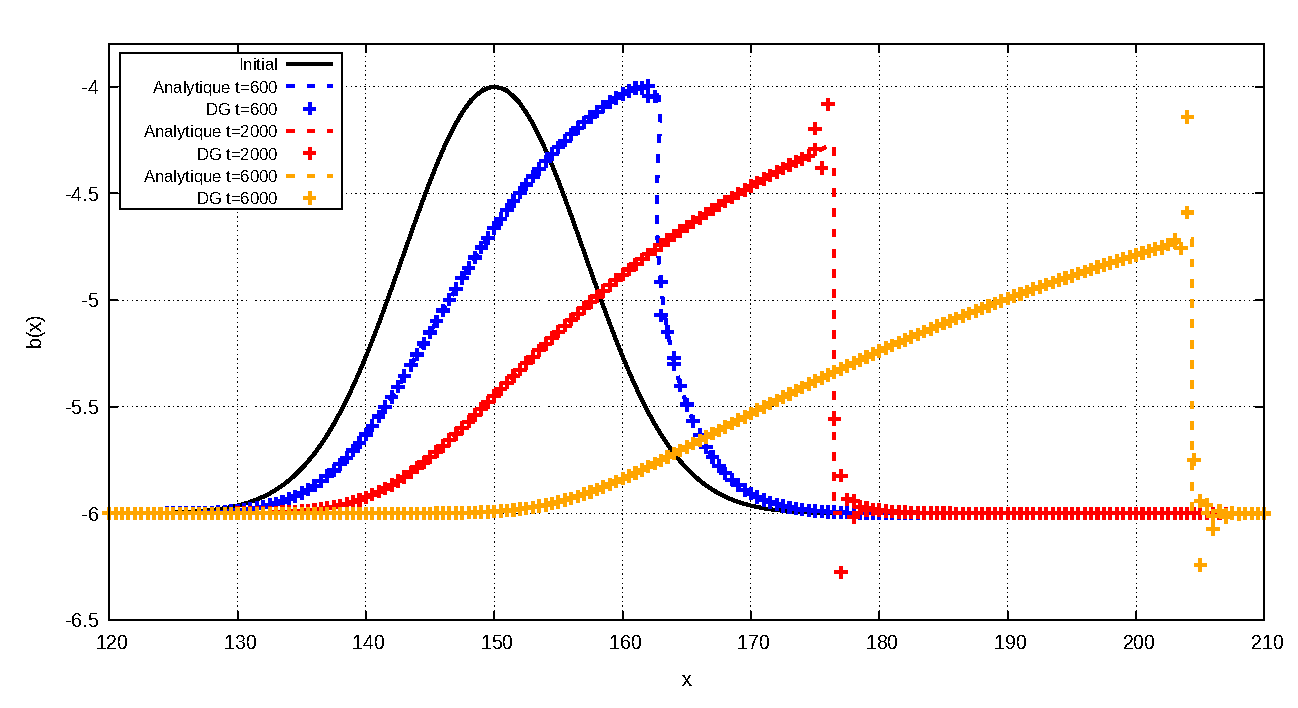
\includegraphics[width=\linewidth]{PNG/Long/long_n_x_300_sans_limiteur.pdf}
        \caption{Solution numérique obtenue sans limiteur de pente}
        \label{fig:long_sans_limiteur}
    \end{subfigure}

    \vspace{0.3cm} % Espace vertical pour séparer nettement les deux grands graphiques

    % --- Deuxième ligne : Avec limiteur (Pleine largeur) ---
    \begin{subfigure}[b]{0.98\linewidth}
        \centering
        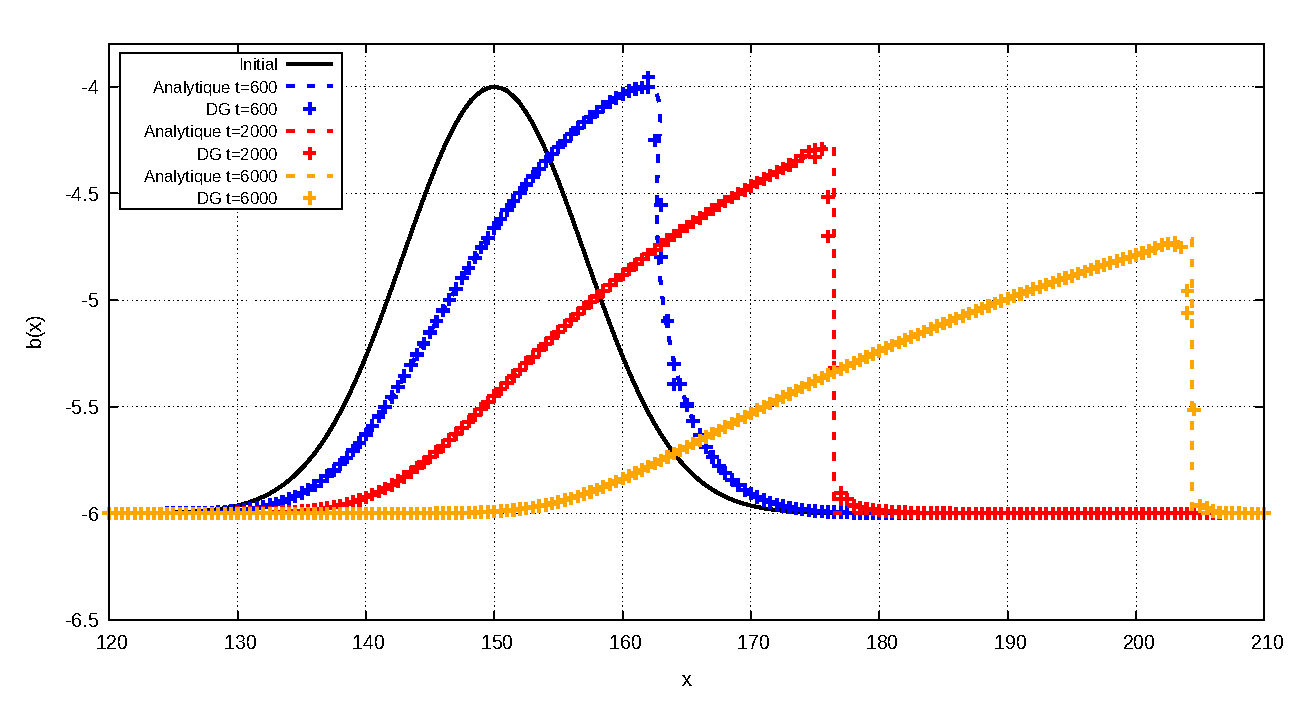
\includegraphics[width=\linewidth]{PNG/Long/long_n_x_300_avec_limiteur.pdf}
        \caption{Solution numérique obtenue avec le limiteur de pente de Krivodonova ($\alpha_i = 1$)}
        \label{fig:long_avec_limiteur}
    \end{subfigure}

    \caption{Cas test 3 -- Comparaison entre les solutions numériques (croix) sans et avec limiteur de pente et la solution semi-analytique (traits) pour $p = 2$ et $N_x = 300$}
    \label{fig:impact_limiteur_long}
\end{figure}

D'un point de vue qualitatif, les solutions numériques approchent avec une grande précision la solution exacte dans les zones régulières. En revanche, la capture du choc dépend fortement de l'activation ou non du limiteur de pente. \\
Par ailleurs, cette comparaison permet de mettre en lumière deux caractéristiques fondamentales du schéma. D'une part, on observe graphiquement la signature structurelle des méthodes DG : à une même interface, la solution numérique peut posséder deux valeurs distinctes.
D'autre part, le limiteur de pente a tendance à diffuser le choc dans la mesure où nous voyons des points plus équitablement répartis à la discontinuité.

Enfin, concernant la conservation globale de la masse sédimentaire en double précision, on observe un écart de $6.65 \times 10^{-9}$ au temps final $t = \SI{6000}{\second}$. \\
Afin de vérifier la nature strictement conservative du schéma, le calcul a été exécuté en quadruple précision. L'écart de masse chute alors à $8.30 \times 10^{-29}$, ce qui correspond au zéro machine pour ce niveau de précision après plusieurs milliers d'itérations. \\
Ce résultat démontre que le schéma est théoriquement conservatif. L'écart observé en double précision est ainsi entièrement dû à la propagation des erreurs d'arrondi numérique sur l'ensemble de la simulation.

\subsection{Cas test 4 : Solution semi-analytique de Fernandez-Nieto \textit{et al.}} \label{sec:Cas_test_2_4}

Ce dernier cas test s'inscrit dans une logique de pré-couplage avec les équations de Saint-Venant. \\
En s'appuyant sur les travaux de Fernandez-Nieto \textit{et al.} \cite{fernandez2025third}, une solution semi-analytique du système de Saint-Venant-Exner 1D peut être établie. \\
Cette dérivation repose sur l'hypothèse d'un flux sédimentaire $G$ régi par la loi de Grass, ainsi que sur une structure spécifique du triplet de conditions initiales $W_\text{ini} = (h_\text{ini}, u_\text{ini}, b_\text{ini})$, définie par
\begin{equation}
    h_\text{ini}(x) = h_0 \in \mathbb{P}^0, \quad u_\text{ini}(x) = A_{FN} x + B_{FN} \in \mathbb{P}^1, \quad b_\text{ini}(x) = \frac{3 \xi_0 A_G A_{FN}}{C_{FN}} u_\text{ini}^2(x) \in \mathbb{P}^2
\end{equation}
où $\xi_0 = 1/(1 - \varepsilon_0)$, $h_0 > 0$, $A_{FN}$, $B_{FN}$, $C_{FN}$ sont des constantes et l'exposant de Grass est fixé à $m_G = 3$. \\
Dès lors, si $\displaystyle \widetilde{W}(t) = \left( \widetilde{h}(t), \widetilde{u}(t), \widetilde{b}(t) \right)$ est une solution du problème
\begin{equation} \label{eq:Fernandez_Nieto_EDO}
    \left \{
    \begin{aligned}
        & \frac{\text{d}}{\text{d}t} \widetilde{h}(t) + A_{FN} \widetilde{u}(t) \widetilde{h}(t) = 0 \\
        & \frac{\text{d}}{\text{d}t} \widetilde{u}(t) + A_{FN} \widetilde{u}^2(t) + \frac{6 g \xi_0 A_G A_{FN}^2}{C_{FN}} \widetilde{b}(t) = 0 \\
        & \frac{\text{d}}{\text{d}t} \widetilde{b}(t) + C_{FN} \widetilde{u}^3(t) = 0 \\
        & \widetilde{\bm{W}}(0) = (h_0, 1, 1)
    \end{aligned}
    \right .
\end{equation}
alors
\begin{equation}
    \bm{W}(x, t) = \left( \widetilde{h}(t), u_\text{ini}(x) \widetilde{u}(t), b_\text{ini}(x) \widetilde{b}(t) \right)
\end{equation}
est une solution du système de Saint-Venant-Exner 1D muni d'une condition aux limites de Dirichlet à gauche, d'une condition aux limites de sortie libre à droite et de la condition initiale $\bm{W}(x, 0) = \bm{W}_\text{ini}(x)$. \\

Par construction, la solution semi-analytique de Fernandez-Nieto \textit{et al.} entraîne naturellement une résolution fortement couplée des équations \eqref{eq:Saint_Venant_Exner}, i.e. le vecteur d'état $\bm{W}$ contient aussi la hauteur de la bathymétrie $b$. \\
Par conséquent, la résolution de \eqref{eq:Fernandez_Nieto_EDO} est, en première approche, effectuée par couplage fort. Cela se traduit par l'extension des routines de reconstruction aux interfaces, du flux numérique de Rusanov, ainsi que du schéma d'intégration temporelle à un système unifié de trois équations différentielles ordinaires. \\
Cependant, nous aimerions garder une structure pleinement modulaire au sein de RIVAGE, laissant alors le choix à l'utilisateur de résoudre le système couplé Saint-Venant-Exner ou seulement les équations de Saint-Venant. \\
En ce sens, on souhaiterait, en seconde approche, transitionner vers un couplage faible pour la résolution de \eqref{eq:Saint_Venant_Exner}.

Une première option consisterait en une résolution purement découplée, où les modules hydrodynamique et morphodynamique sont intégrés séparément à chaque pas de temps en utilisant les grandeurs figées $b^n$ et $(h^n, u^n)$. \\
Néanmoins, cette approche par décomposition d'opérateurs (\textit{splitting}) s'avère inadaptée : d'une part, elle introduit un déphasage numérique important dégradant la précision de la solution, et d'autre part, elle brise l'ordre élevé du schéma d'intégration temporelle.

Une deuxième possibilité serait d'employer une résolution faiblement couplée à l'aide d'un schéma de Runge-Kutta IMEX : pour un stade $s$ de la discrétisation temporelle, \eqref{eq:Saint_Venant} est résolu de manière explicite, puis l'équation \eqref{eq:Exner_generalisee} est résolue de manière implicite en utilisant le vecteur d'état hydrodynamique tout juste calculé $(h^{(s)},u^{(s)})$. \\
Cette approche résoudrait directement les deux défauts majeurs de la première stratégie : d'une part, elle ne présente aucun déphasage puisque la bathymétrie intervenant dans le terme source de Saint-Venant est réévaluée à chaque sous-pas de temps ; d'autre part, il existe dans la littérature des schémas IMEX d'ordre élevé bien documentés. \\
Toutefois, comme souligné en début de la section \ref{sec:Formulation_discrete_1D}, la résolution purement implicite de l'équation d'Exner s'avère très coûteuse numériquement. De plus, le rayon de contractivité des méthodes itératives étant particulièrement restreint dans notre configuration, rien ne garantit que le pas de temps dicté par la condition CFL explicite de Saint-Venant soit suffisamment petit pour assurer la convergence du solveur implicite d'Exner.

Une dernière alternative, inspirée de la précédente, consisterait à traiter de manière explicite le système \eqref{eq:Saint_Venant} ainsi que le flux $G$. Le terme source de l'équation d'Exner pourrait quant à lui être traité en explicite ou en implicite, selon sa raideur propre. \\
Plus précisément, pour chaque étape $s$ du schéma temporel, on résout de manière synchrone les équations de Saint-Venant et l'équation d'Exner, avant d'utiliser ces solutions comme données d'entrée à l'étape suivante. \\
Cette proposition apparaît comme la meilleure alternative : elle permet de conserver une structure découplée pour le vecteur d'état et la bathymétrie, tout en minimisant les erreurs de déphasage. De plus, elle préserve l'ordre élevé et les schémas SSP détaillés dans la section \ref{sec:Formulation_discrete_1D}. Le seul inconvénient réside dans l'obligation de maintenir une discrétisation temporelle identique pour les deux EDO issues de la semi-discrétisation. Cela reste \textit{a priori} un faux problème, car il apparaît plus cohérent d'avoir une résolution au même ordre temporel pour ces deux équations, étant donné que l'erreur globale du système couplé est limitée par le schéma le moins précis. \\

On peut remarquer que cette dernière possibilité est très proche d'un couplage fort pour la résolution du système \eqref{eq:Saint_Venant_Exner}. De fait, \textit{a priori}, la seule différence réside dans le calcul des valeurs propres pour \eqref{eq:Saint_Venant} : le couplage fort induit une troisième valeur propre au sein du système, liée à la vitesse de propagation de l'onde sédimentaire (voir par exemple \cite{fernandez2025third}). \\
En revanche, la dernière option, que l'on qualifiera de faiblement couplée par la suite, dissocie les flux numériques en évitant d'intégrer cette troisième valeur propre dans le flux de Rusanov hydrodynamique. Ce choix est particulièrement pertinent pour RIVAGE : il permet de conserver notre solveur RKDG, là où un couplage fort imposerait un solveur de Riemann complet intégrant les trois ondes du système. \\
On peut aussi ajouter que la vitesse de l'onde sédimentaire n'entre plus en jeu dans la condition CFL de Saint-Venant (si l'on choisit l'approximation de De Vries \cite{vries1965considerations}) ; par conséquent, le pas de temps pour la résolution faiblement couplée pourra être choisi comme étant le plus faible entre le pas de temps de \eqref{eq:Saint_Venant} et celui de l'équation \eqref{eq:Exner_generalisee} (à un facteur de sûreté près). \\
Enfin, on peut noter que, pour ce cas test précis, comme nous disposons pour l'instant seulement d'un solveur RKDG pour l'équation d'Exner, la résolution faiblement couplée et la résolution totalement couplée sont algébriquement équivalentes. \\
Il sera donc pertinent de reprendre ce cas test lors de l'implémentation de notre module dans RIVAGE pour vérifier la consistance en ordre et en erreur.

Les cas tests 1 et 3 sont construits de sorte à faire intervenir une dépendance explicite en $b$ pour la vitesse $u$ et le cas test 2 est suffisamment lisse pour qu'un flux centré soit stable pour le schéma RKDG. \\
Cependant, dans le cas général, le flux $G$ ne dépend pas explicitement de $b$ (de sorte que $\partial_b G = 0$), ce qui est par exemple le cas de la loi de Grass. La dépendance par rapport au fond devient indirecte et dictée par la réponse de l'hydrodynamique. \\
Dans cette configuration, la vitesse de l'onde sédimentaire $\lambda_i^n$ ne peut plus être obtenue directement par la formule \eqref{eq:Vitesse_onde_sedimentaire}. Elle doit alors être exprimée à partir des valeurs propres de la Jacobienne associée à l'écriture sous forme vectorielle non conservative de \eqref{eq:Saint_Venant_Exner}. \\
Par linéarisation, on obtient la vitesse caractéristique locale de l'onde sédimentaire de De Vries
\begin{equation}
    \lambda_{i, \text{DV}}(x, t) = \frac{1}{m \left( \bm{\Phi}_i^T(x) \bm{\beta}_i(t) \right)} \left| \partial_q G \left( \bm{\Phi}_i^T(x) \bm{B}_i(t) \right) \frac{u(x, t)}{1 - \text{Fr}^2} \right|
\end{equation}
où $u(x, t) = u_\text{ini}(x) \widetilde{u}(t)$ et Fr est le nombre de Froude. \\
Par identification avec $\lambda_i^n$, le coefficient de diffusion du flux de Rusanov à l'interface située en $x_{i+\sfrac{1}{2}}$ s'écrit alors
\begin{equation}
    \alpha_{i + \sfrac{1}{2}} = \max \left( \left| \partial_q G \left( \bm{\Phi}_i^T(1) \bm{B}_i(t) \right) \frac{u(x_{i + \sfrac{1}{2}}, t)}{1 - \text{Fr}^2} \right|, \left| \partial_q G \left( \bm{\Phi}_{i+1}^T(-1) \bm{B}_{i+1}(t) \right) \frac{u(x_{i + \sfrac{1}{2}}, t)}{1 - \text{Fr}^2} \right| \right)
\end{equation}
En outre, la stabilité globale du schéma nécessite également de prendre en compte les vitesses caractéristiques des ondes de Saint-Venant pour ce cas test. \\
On introduit ainsi la vitesse d'onde maximale
\begin{equation}
    \lambda_{i, \text{max}} = \max_{F \in \partial \Omega_i^n} \left( \max_{x \in F} \left( \left| u(x, t^n) - \sqrt{g h} \right|, \lambda_{i, \text{DV}}(x, t^n), \left| u(x, t^n) + \sqrt{g h} \right| \right) \right)
\end{equation}
Par conséquent, la condition CFL pour le pas de temps lié à l'advection est donnée par
\begin{equation}
    \max_{1 \leq i \leq N_x} \left( \frac{\lambda_{i, \text{max}}}{\Delta x_i} \right) \Delta t^A \leq \frac{1}{2p + 1}
\end{equation}
Le pas de temps global est alors défini selon \eqref{eq:Pas_de_temps_Exner} par
\begin{equation}
    \Delta t^n = \alpha_\text{CFL} \min \left( \Delta t^A, \Delta t^S \right)
\end{equation}
où $\Delta t^S$ est le pas de temps lié au terme source défini en \eqref{eq:Pas_de_temps_source_Exner}. \\
L'établissement détaillé des valeurs propres de De Vries sera présenté dans la troisième partie, celle-ci nécessitant l'introduction préalable du système couplé \eqref{eq:Saint_Venant_Exner}.

Enfin, les constantes sont fixées conformément à l'article de Fernandez-Nieto \textit{et al.} afin d'avoir une comparaison qualitative des résultats. \\
Ainsi, on a les paramètres
\begin{equation}
    h_0 = 10, \quad A_{FN} = 0.01, \quad B_{FN} = 0.01, \quad C_{FN} = \xi_0 = 1, \quad A_G = 0.001
\end{equation}
De plus, par construction, la solution exacte pour la hauteur de la bathymétrie $b(x, t)$ est un polynôme de degré 2 en espace. En ce sens, utiliser un degré polynomial $p = 2$ pour l'espace DG n'aurait d'autre intérêt que de mesurer l'erreur intrinsèque de notre schéma. \\
Par conséquent, la figure \ref{fig:Comparaison_Fernandez_Nieto} ainsi que le tableau de convergence \ref{tab:convergence_fernandez_nieto} sont obtenus en fixant $p = 1$. \\
Par ailleurs, ce cas test permettra également de vérifier l'hypothèse établie lors du cas test précédent : l'erreur obtenue sur la masse totale en fin de simulation demeure uniquement liée aux erreurs d'arrondis accumulées au cours du calcul.

\begin{figure} [!t]
    \centering
    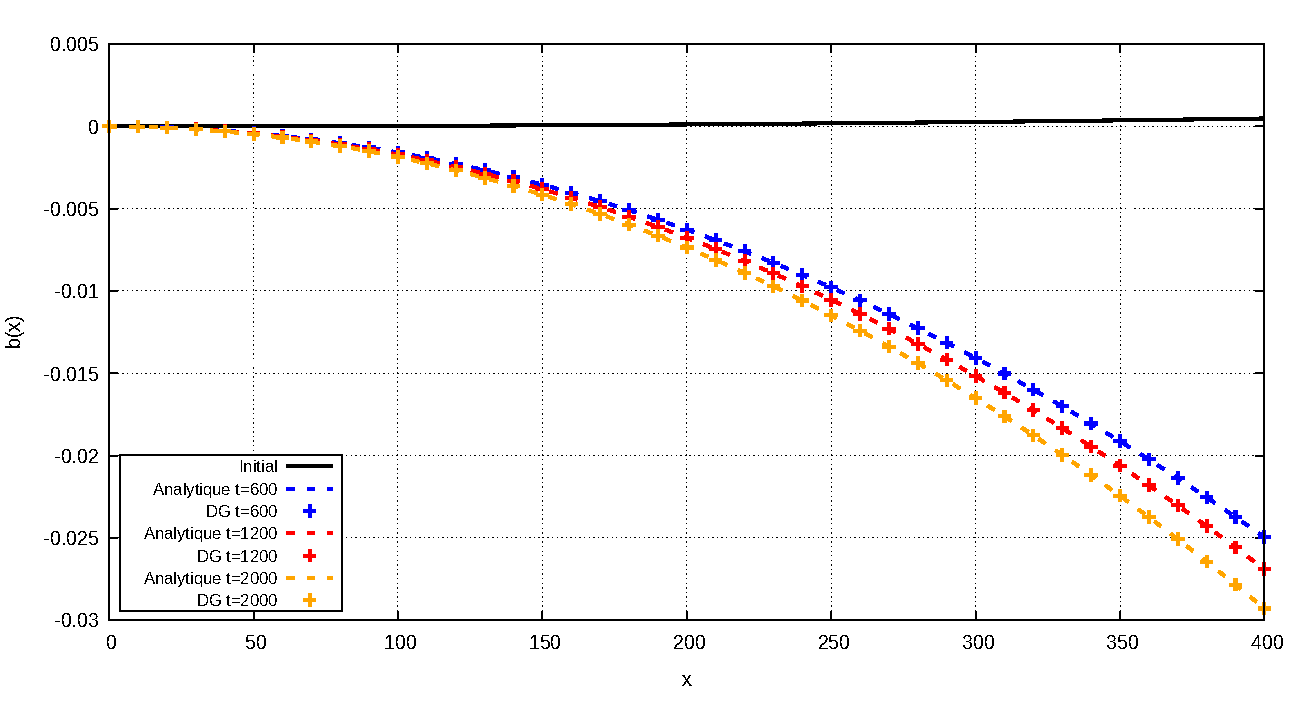
\includegraphics[width=0.96\linewidth]{PNG/Fernandez_Nieto/fernandez_nieto_n_x_40.pdf}
    \caption{Cas test 4 -- Comparaison entre la solution numérique (croix) et la solution semi-analytique (traits) à différents instants pour $p = 1$ et $N_x = 40$}
    \label{fig:Comparaison_Fernandez_Nieto}
\end{figure}

Qualitativement, la solution numérique concorde avec la solution semi-analytique exacte, validant ainsi notre implémentation vis-à-vis de \cite{fernandez2025third}. Sur le plan quantitatif, les erreurs en normes $L^2$ et $L^\infty$, ainsi que l'ordre de convergence associé, sont rassemblés dans le tableau \ref{tab:convergence_fernandez_nieto}. On y retrouve bien l'ordre théorique optimal du schéma DG, à savoir $p+1 = 2$.

\begin{table}[H]
    \centering
    \small
    \begin{tabular}{r ccc}
    \toprule
    $N_x$ & $L^2$ & $L^\infty$ & Ordre \\
    \midrule
    10 & 4.34E-04 & 2.97E-05 & -- \\
    20 & 1.08E-04 & 7.34E-06 & 2.00 \\
    40 & 2.71E-05 & 1.85E-06 & 1.99 \\
    80 & 6.79E-06 & 4.64E-07 & 1.99 \\
    \bottomrule
    \end{tabular}
    \caption{Cas test 4 -- Erreurs d'approximation en norme $L^2$, $L^\infty$ au temps $t = \SI{2000}{\second}$ et ordres de convergence associés pour $p = 1$}
    \label{tab:convergence_fernandez_nieto}
\end{table}

Pour finir, en fixant $p = 2$, l'erreur obtenue est de $1.59 \times 10^{-9}$ au temps $t = \SI{2000}{\second}$, un ordre de grandeur similaire à l'erreur sur la masse du cas test 3. Cette configuration permet d'isoler précisément les sources d'erreur numérique.

D'une part, la détermination des points de quadrature de Gauss repose sur la recherche des racines du polynôme de Legendre de degré $k$. Cette étape utilise une méthode de Newton dont le critère d'arrêt est fixé à $\varepsilon_\text{racine} = 10^{-10}$. D'autre part, l'inversion de chaque bloc $\mathbb{M}_i$ de la matrice de masse est réalisée par un algorithme de Cholesky, celle-ci étant dense lorsque la fonction $m$ n'est pas constante. Un second critère de tolérance, noté $\varepsilon_\text{var} = 10^{-12}$, est introduit pour définir le zéro machine.

En resserrant ces deux critères à $10^{-14}$, l'erreur intrinsèque obtenue chute à $3.44 \times 10^{-13}$ en norme $L^2$, démontrant que la quasi-totalité de l'erreur initiale provient de ces deux seuils de convergence. Le reliquat peut alors être attribué aux erreurs d'arrondis accumulées au cours du calcul, compte tenu des 15520 pas de temps effectués pour $p = 2$ et $N_x = 40$. \\
Enfin, une simulation menée en quadruple précision avec les seuils $\varepsilon_\text{racine} = \varepsilon_\text{var} = 10^{-32}$ conduit à une erreur de $2.73 \times 10^{-32}$, validant ainsi de manière définitive la conservation stricte de la masse et l'exactitude de la quadrature numérique.

\section{Formulation semi-discrète 2D}

Nous pouvons désormais nous intéresser à l'extension en 2D de notre problème. \\
Sur la base des notations déjà introduites, on considère un domaine $\Omega$ ouvert convexe de $\mathbb{R}^2$. Le maillage de $\Omega$ au temps $t^n$, noté $\mathcal{M}^n$, est composé de $N_e$ éléments notés $\Omega_i^n$. \\
On note $\widehat{\Omega}$ la maille de référence et $\widehat{F} = [-1, 1]$ la face de référence. Comme on s'intéresse à des maillages non structurés de quadrilatères ou de triangles, l'élément de référence change selon la forme des mailles : si les mailles sont rectangulaires, alors
\begin{equation}
    \widehat{\Omega} = \mathcal{Q} = \left\{ (x, y) \in \mathbb{R}^2 : -1 \leq x \leq 1, ~ -1 \leq y \leq 1 \right\}
\end{equation}
et si les mailles sont triangulaires, alors
\begin{equation}
    \widehat{\Omega} = \mathcal{T} = \left\{ (x, y) \in \mathbb{R}^2 : 0 \leq x, y \leq 1, ~ 0 \leq x + y \leq 1 \right\}
\end{equation}

Si le maillage $\mathcal{M}^n$ est conforme (i.e. aucune maille $\Omega_i^n$ n'est plate), alors il existe une application $\widehat{\phi}_i(\xi, \eta) : \widehat{\Omega} \longrightarrow \Omega_i^n$ qui envoie l'élément de référence sur la maille $\Omega_i^n$ et son inverse $\widehat{\phi}_i^{-1}(x, y) : \Omega_i^n \longrightarrow \widehat{\Omega}$ mappant les coordonnées de la maille $\Omega_i^n$ vers l'élément de référence $\widehat{\Omega}$. \\
De plus, on introduit aussi $\widehat{\phi}_F(\xi) : \widehat{F} \longrightarrow F$ l'application envoyant la face de référence $\widehat{F}$ sur la face physique $F$. Comme nous travaillons en 2D, l'inverse de cette application n'est pas défini, mais c'est un faux problème car, en DG, les faces ne contiennent pas d'informations sur les inconnues, seuls les éléments en contiennent. \\
En particulier, pour deux nœuds d'une face $F$, de coordonnées $(x_1, y_1)$ et $(x_2, y_2)$, l'application $\widehat{\phi}_F$ est définie par
\begin{equation}
    \forall \xi \in \widehat{F}, ~ \widehat{\phi}_F(\xi) = \begin{pmatrix} x_1 & x_2 \\ y_1 & y_2 \end{pmatrix} \begin{pmatrix} (1 - \xi)/2 \\ (1 + \xi)/2 \end{pmatrix}
\end{equation}
Ainsi, on peut introduire le changement de variable d'une face $F$ vers la face de référence $\widehat{F}$ : si $g : F \longrightarrow \mathbb{R}$, alors
\begin{equation}
    \int_F g(x, y) \text{d}F = \int_{\widehat{F}} g(\widehat{\phi}_F(\xi)) \lvert F \rvert \text{d}\widehat{F}
\end{equation}
avec $\lvert F \rvert = \sqrt{(x_2 - x_1)^2 + (y_2 - y_1)^2}/2$ le Jacobien du changement de variable.

Enfin, la base de l'espace des polynômes de degré au plus $p_i$ diffère elle aussi selon la forme des mailles. \\
D'une part, si $\Omega_i^n$ est un parallélogramme, alors on utilise la base de Legendre 2D, construite par produit tensoriel des polynômes de Legendre 1D, soit
\begin{equation}
    \LegendreL_{k, m}(\xi, \eta) = c_k \mathcal{L}_k(\xi) c_m \mathcal{L}_m(\eta), ~ 0 \leq k, m \leq p_i
\end{equation}
avec $\mathcal{L}_k$ le polynôme de Legendre de degré $k$ et $c_k = \sqrt{(2k+1)/2}$ sa constante de normalisation. \\
D'autre part, si $\Omega_i^n$ est un triangle, alors on utilise la base de Dubiner \cite{dubiner1991spectral}, construite à partir des polynômes de Legendre et de Jacobi, de sorte que
\begin{equation}
    \DubinerD_{k, m}(\xi, \eta) = C_{k, m} 2^k \mathcal{L}_k \left( \frac{2 \eta}{1 - \xi} - 1 \right) (1 - \xi)^k \mathcal{P}_m^{(2k+1, 0)}(2 \xi - 1), ~ 0 \leq k + m \leq p_i
\end{equation}
où $C_{k, m}$ est une constante de normalisation et $\mathcal{P}_m^{(2k+1, 0)}$ est le polynôme de Jacobi de degré $m$ et de paramètres $(2k+1, 0)$. \\
De même qu'en 1D, ce choix est justifié par l'orthogonalité de ces deux bases pour le produit scalaire de $L^2(\mathcal{Q})$ et $L^2(\mathcal{T})$, ainsi que par leur caractère hiérarchique, permettant alors de choisir le degré polynomial au sein de chaque maille sans devoir générer à nouveau ces deux bases. \\
Pour finir l'introduction des notations, on note $N_\text{ddl}^i$ le nombre de degrés de liberté de la maille $\Omega_i^n$ tel que
\begin{equation}
    N_\text{ddl}^i =
    \left \{
    \begin{aligned}
        &(p_i + 1)^2                &&\text{si } \widehat{\Omega} = \mathcal{Q} \\
        &\frac{(p_i+1)(p_i+2)}{2}   &&\text{si } \widehat{\Omega} = \mathcal{T}
    \end{aligned}
    \right .
\end{equation}

L'expression de la formulation variationnelle en 2D pour le problème \eqref{eq:Exner_generalisee} est tout à fait semblable à \eqref{eq:Probleme_variationnel_exner_1D} : on multiplie l'équation d'Exner par une fonction test de $\mathcal{V}^{\mathbf{p}}(\mathcal{M}^n)$, puis on applique la formule de la divergence. \\
Ainsi, on cherche à résoudre le problème variationnel
\begin{equation} \tag{$\mathcal{P}_{SD}^{\mathcal{E}}$} \label{eq:Probleme_variationnel_exner}
    \left \{
    \begin{aligned}
        & \text{Trouver } b_h \in \mathcal{V}^\mathbf{p}(\mathcal{M}^n) \text{ tel que } \forall \varphi \in \mathcal{V}^\mathbf{p}(\mathcal{M}^n) \\
        & m_\mathcal{E}^n(\partial_t b_h, \varphi; b_h) + a_\mathcal{E}^n(\varphi; b_h) = l_\mathcal{E}^n (\varphi)
    \end{aligned}
    \right .
\end{equation}
où les applications DG $m_\mathcal{E}^n$ et $a_\mathcal{E}^n$, et la forme linéaire $l_\mathcal{E}^n$ sont définies comme
\begin{equation}
    \begin{aligned}
        \forall v_1, v_2, \varphi \in \mathcal{V}^\mathbf{p}(\mathcal{M}^n), ~ &m_\mathcal{E}^n(v_1, \varphi; v_2) = \sum_{\Omega_i^n \in \mathcal{M}^n} \int_{\Omega_i^n} m(\nabla v_2) v_1 \varphi \text{d}\bm{x} \\
        & a_\mathcal{E}^n(\varphi; v_1) = - \sum_{\Omega_i^n \in \mathcal{M}^n} \int_{\Omega_i^n} \bm{G}(v_1) \cdot \nabla \varphi \text{d}\bm{x} - \sum_{\Omega_i^n \in \mathcal{M}^n} \int_{\Omega_i^n} S(v_1) \varphi \text{d}\bm{x} \\
        & \phantom{a_\mathcal{E}^n(\varphi; v_1) = } - \sum_{F \in \mathcal{F}^\text{int}} \int_F \left( \bm{\widehat{G}}_F \cdot \bm{n}_F \right) \llbracket \varphi \rrbracket \text{d}F \\
        & l_\mathcal{E}^n(\varphi) = - \sum_{F \in \mathcal{F}_D^\partial} \int_F \left( \bm{\widehat{G}}_F(b_D) \cdot \bm{n}_F \right) \varphi \text{d}F - \sum_{F \in \mathcal{F}_N^\partial} \int_F \bm{q}_N \varphi \text{d}F
    \end{aligned}
\end{equation}
Cette formulation variationnelle est équivalente à la formulation matricielle locale
\begin{equation} \tag{$\mathcal{P}_M^\mathcal{E}$} \label{eq:Probleme_matriciel_exner}
    \left \{
    \begin{aligned}
        & \forall i \in \llbracket 1, N_e \rrbracket \text{ trouver } \bm{B}_i \in \mathbb{R}^{N_\text{ddl}^i} \text{ tel que } \\
        & \mathbb{M}_i(t) \partial_t \bm{B}_i(t) = \bm{\mathcal{I}}_i^{EF}(t) - \bm{\mathcal{I}}_i^{VF}(t) + \bm{\mathcal{I}}_i^S(t) \\
        & \bm{B}_i(0) = \bm{B}_i^0
    \end{aligned}
    \right .
\end{equation}
avec
\begin{itemize}
    \item $\displaystyle \mathbb{M}_i(t) = \int_{\widehat{\Omega}} m \left( \mathbb{D}_i^T(\xi, \eta) \bm{\beta}_i(t) \right) \bm{\Phi}_i(\xi, \eta) \bm{\Phi}_i^T(\xi, \eta) \lvert \Omega_i^n \rvert \text{d}\widehat{\Omega} \in \mathbb{R}^{N_\text{ddl}^i \times N_\text{ddl}^i}$ la matrice de masse
    \item $\displaystyle \bm{\mathcal{I}}_i^{EF}(t) = \int_{\widehat{\Omega}} \widetilde{\nabla}_i \bm{\Phi}_i(\xi, \eta) \cdot \bm{G} \left( \bm{\Phi}_i^T(\xi, \eta) \bm{B}_i(t) \right) \lvert \Omega_i^n \rvert \text{d}\widehat{\Omega} \in \mathbb{R}^{N_\text{ddl}^i}$ le vecteur de contribution volumique du flux
    \item $\displaystyle \bm{\mathcal{I}}_i^{VF}(t) = \sum_{F \in \partial \Omega_i^n} \int_{\widehat{F}} \left( \bm{\widehat{G}}_F \cdot \bm{n}_F \right) \bm{\Phi}_F(\xi) \lvert F \rvert \text{d}\widehat{F} \in \mathbb{R}^{N_\text{ddl}^i}$ le vecteur de contribution du flux aux interfaces
    \item $\displaystyle \bm{\mathcal{I}}_i^S(t) = \int_{\widehat{\Omega}} \bm{\Phi}_i(\xi, \eta) S \left( \bm{\Phi}_i^T(\xi, \eta) \bm{B}_i(t) \right) \lvert \Omega_i^n \rvert \text{d}\widehat{\Omega} \in \mathbb{R}^{N_\text{ddl}^i}$ le vecteur de contribution volumique du terme source
\end{itemize}
où nous avons défini
\begin{equation}
    \lvert \Omega_i^n \rvert = \left| \text{det}\left( \mathbb{J}_i(\xi, \eta) \right) \right| \quad \text{et} \quad \widetilde{\nabla}_i = \left( \mathbb{J}_i^{-1}(\xi, \eta) \right)^T \begin{pmatrix} \partial_\xi \\ \partial_\eta \end{pmatrix}
\end{equation}
avec $\mathbb{J}_i$ la matrice Jacobienne associée à la règle de la chaîne lors du changement de variable $\bm{x} = \widehat{\phi}_i(\xi, \eta)$. \\
De plus, $\bm{\Phi}_F \in \mathbb{R}^{N_\text{ddl}^i}$ est le vecteur contenant la base de l'espace polynomial $\mathbb{P}^{p_i}(\Omega_i^n)$ évaluée sur la face $F$, de telle sorte que
\begin{equation}
    \bm{\Phi}_F(\xi) = \bm{\Phi}_i \left( \gamma_F(\xi) \right)
\end{equation}
où, pour deux sommets $(\xi_1, \eta_1)$ et $(\xi_2, \eta_2)$ de l'élément de référence $\widehat{\Omega}$, la trace $\gamma_F$ de la face $F$ est donnée par
\begin{equation}
    \forall \xi \in \widehat{F}, \quad \gamma_F(\xi) = \frac{1-\xi}{2} \begin{pmatrix} \xi_1 \\ \eta_1 \end{pmatrix} + \frac{1+\xi}{2} \begin{pmatrix} \xi_2 \\ \eta_2 \end{pmatrix}
\end{equation}
Enfin, $\bm{\beta}_i = (\bm{\beta}_{i, x}, \bm{\beta}_{i, y}) \in \mathbb{R}^{2N_\text{ddl}^i}$ est le vecteur de modes associé à la projection de $\nabla b$ sur $\left[ \mathcal{V}^\mathbf{p}(\mathcal{M}^n) \right]^2$. \\
De même qu'en 1D, on cherche à résoudre le problème
\begin{equation}
    \left \{
    \begin{aligned}
        &\text{Trouver } \bm{\beta}_h = (\beta_{h, x}, \beta_{h, y}) \in \left[ \mathcal{V}^\mathbf{p}(\mathcal{M}^n) \right]^2 \text{ tel que } \forall \varphi \in \mathcal{V}^\mathbf{p}(\mathcal{M}^n) \\
        &\sum_{\Omega_i^n \in \mathcal{M}^n} \int_{\Omega_i^n} (\nabla b) \varphi \text{d}\bm{x} = \sum_{\Omega_i^n \in \mathcal{M}^n} \int_{\Omega_i^n} \bm{\beta}_h \varphi \text{d}\bm{x}
    \end{aligned}
    \right .
\end{equation}
En décomposant le problème suivant $e_x = (1, 0)$ et $e_y = (0, 1)$ et en appliquant la formule de la divergence, on obtient le problème matriciel
\begin{equation} \label{eq:Beta_Exner_2D}
    \left \{
    \begin{aligned}
        & \forall i \in \llbracket 1, N_e \rrbracket \text{ trouver } \bm{\beta}_{i, x}, \bm{\beta}_{i, y} \in \mathbb{R}^{N_\text{ddl}^i} \text{ tels que} \\
        & - \mathbb{K}_{i, x}^\text{std} \bm{B}_i(t) + \sum_{F \in \partial \Omega_i^n} \int_{\widehat{F}} \left( \widehat{b}_F \cdot n_{F, x} \right) \bm{\Phi}_F(\xi) \lvert F \rvert \text{d}\widehat{F} = \mathbb{M}_i^\text{std} \bm{\beta}_{i, x}(t) \\
        & - \mathbb{K}_{i, y}^\text{std} \bm{B}_i(t) + \sum_{F \in \partial \Omega_i^n} \int_{\widehat{F}} \left( \widehat{b}_F \cdot n_{F, y} \right) \bm{\Phi}_F(\xi) \lvert F \rvert \text{d}\widehat{F} = \mathbb{M}_i^\text{std} \bm{\beta}_{i, y}(t) \\
    \end{aligned}
    \right .
\end{equation}
avec
\begin{itemize}
    \item $\displaystyle \mathbb{M}_i^\text{std} = \int_{\widehat{\Omega}} \bm{\Phi}_i(\xi, \eta) \bm{\Phi}_i^T(\xi, \eta) \lvert \Omega_i^n \rvert \text{d}\widehat{\Omega} \in \mathbb{R}^{N_\text{ddl}^i \times N_\text{ddl}^i}$ le bloc correspondant à la maille $\Omega_i^n$ de la matrice de masse standard
    \item $\displaystyle \mathbb{K}_{i, x}^\text{std} = \int_{\widehat{\Omega}} \left( \widetilde{\nabla}_i \bm{\Phi}_i(\xi, \eta) \cdot e_x \right) \bm{\Phi}_i^T(\xi, \eta) \lvert \Omega_i^n \rvert \text{d}\widehat{\Omega} \in \mathbb{R}^{N_\text{ddl}^i \times N_\text{ddl}^i}$ la composante $x$ du bloc correspondant à la maille $\Omega_i^n$ de la matrice de rigidité standard
    \item $\displaystyle \mathbb{K}_{i, y}^\text{std} = \int_{\widehat{\Omega}} \left( \widetilde{\nabla}_i \bm{\Phi}_i(\xi, \eta) \cdot e_y \right) \bm{\Phi}_i^T(\xi, \eta) \lvert \Omega_i^n \rvert \text{d}\widehat{\Omega} \in \mathbb{R}^{N_\text{ddl}^i \times N_\text{ddl}^i}$ la composante $y$ du bloc correspondant à la maille $\Omega_i^n$ de la matrice de rigidité standard
    \item $\displaystyle \widehat{b}_F = \frac{1}{2} \left( \bm{\Phi}_{F, i}^T(\xi) \bm{B}_i(t) + \bm{\Phi}_{F, r}^T(\xi) \bm{B}_r(t) \right)$ le flux centré à l'interface $F$ où l'indice $r$ désigne la maille $\Omega_r^n$ adjacente à la maille $\Omega_i^n$ par la face $F$, i.e. $\Omega_i^n \cap \Omega_r^n = F$
\end{itemize}

Le passage de la formulation variationnelle à la formulation matricielle s'effectue naturellement en étendant les notations utilisées en 1D. \\
Ainsi, $b_h$, $\beta_{h, x}$ et $\varphi$ sont projetés sur l'espace DG $\mathcal{V}^\mathbf{p}(\mathcal{M}^n)$ comme
\begin{equation} \label{eq:Projection_DG_Exner_2D}
    \begin{aligned}
        & b_h(\bm{x}, t) = \sum_{i = 1}^{N_e} \mathds{1}_{\Omega_i^n}(\bm{x}) \bm{\Phi}_i^T(\bm{x}) \bm{B}_i(t) &&\text{avec } \bm{\Phi}_i^T, \bm{B}_i \in \mathbb{R}^{N_\text{ddl}^i} \\
        & \beta_{h, x} (\bm{x}, t) = \sum_{i = 1}^{N_e} \mathds{1}_{\Omega_i^n}(\bm{x}) \bm{\Phi}_i^T(\bm{x}) \bm{\beta}_{i, x}(t) &&\text{avec } \bm{\Phi}_i^T, \bm{\beta}_{i, x} \in \mathbb{R}^{N_\text{ddl}^i} \\
        & \varphi(\bm{x}) = \sum_{i = 1}^{N_e} \bm{V}_i^T \mathds{1}_{\Omega_i^n}(\bm{x}) \bm{\Phi}_i(\bm{x}) &&\text{avec } \bm{V}_i^T, \bm{\Phi}_i \in \mathbb{R}^{N_\text{ddl}^i} \\
    \end{aligned}
\end{equation}
Par conséquent, d'une part
\begin{equation}
    \begin{aligned}
        \sum_{\Omega_i^n \in \mathcal{M}^n} \int_{\Omega_i^n} \varphi \beta_{h, x} \text{d}\bm{x} & = \sum_{\Omega_i^n \in \mathcal{M}^n} \bm{V}_i^T \int_{\Omega_i^n} \bm{\Phi}_i(\bm{x}) \bm{\Phi}_i^T(\bm{x}) \text{d}\bm{x} \bm{\beta}_{i, x}(t) \\
        & = \sum_{\Omega_i^n \in \mathcal{M}^n} \bm{V}_i^T \int_{\widehat{\Omega}} \bm{\Phi}_i(\xi, \eta) \bm{\Phi}_i^T(\xi, \eta) \lvert \Omega_i^n \rvert \text{d}\widehat{\Omega} \bm{\beta}_{i, x}(t) \\
        \sum_{\Omega_i^n \in \mathcal{M}^n} \int_{\Omega_i^n} \varphi \beta_{h, x} \text{d}\bm{x} & = \sum_{\Omega_i^n \in \mathcal{M}^n} \bm{V}_i^T \mathbb{M}_i^\text{std} \bm{\beta}_{i, x}(t)
    \end{aligned}
\end{equation}

\noindent
D'autre part,
\begin{equation}
    \begin{aligned}
        & \sum_{\Omega_i^n \in \mathcal{M}^n} \int_{\Omega_i^n} \varphi (\nabla b_h \cdot e_x) \text{d}\bm{x} = - \sum_{\Omega_i^n \in \mathcal{M}^n} \int_{\Omega_i^n} (\nabla \varphi \cdot e_x) b_h \text{d}\bm{x} \\
        & \phantom{\sum_{\Omega_i^n \in \mathcal{M}^n} \int_{\Omega_i^n} \varphi (\nabla b_h \cdot e_x) \text{d}\bm{x} = } + \sum_{\Omega_i^n \in \mathcal{M}^n} \sum_{F \in \partial \Omega_i^n} \int_{F} \varphi \left( \widehat{b}_F \cdot n_{F, x} \right) \text{d}F \\
        & \phantom{\sum_{\Omega_i^n \in \mathcal{M}^n} \int_{\Omega_i^n} \varphi (\nabla b_h \cdot e_x) \text{d}\bm{x}} = - \sum_{\Omega_i^n \in \mathcal{M}^n} \bm{V}_i^T \int_{\Omega_i^n} \left( \nabla \bm{\Phi}_i(\bm{x}) \cdot e_x \right) \bm{\Phi}_i^T(\bm{x}) \text{d}\bm{x} \bm{B}_i(t) \\
        & \phantom{\sum_{\Omega_i^n \in \mathcal{M}^n} \int_{\Omega_i^n} \varphi (\nabla b_h \cdot e_x) \text{d}\bm{x} = } + \sum_{\Omega_i^n \in \mathcal{M}^n} \bm{V}_i^T \sum_{F \in \partial \Omega_i^n} \int_{F} \bm{\Phi}_i(\bm{x}) \left( \widehat{b}_F \cdot n_{F, x} \right) \text{d}F \\
        & \phantom{\sum_{\Omega_i^n \in \mathcal{M}^n} \int_{\Omega_i^n} \varphi (\nabla b_h \cdot e_x) \text{d}\bm{x}} = - \sum_{\Omega_i^n \in \mathcal{M}^n} \bm{V}_i^T \int_{\widehat{\Omega}} \left( \widetilde{\nabla}_i \bm{\Phi}_i(\xi, \eta) \cdot e_x \right) \bm{\Phi}_i^T(\xi, \eta) \lvert \Omega_i^n \rvert \text{d} \widehat{\Omega} \bm{B}_i(t) \\
        & \phantom{ \sum_{\Omega_i^n \in \mathcal{M}^n} \int_{\Omega_i^n} \varphi (\nabla b_h \cdot e_x) \text{d}\bm{x} = } + \sum_{\Omega_i^n \in \mathcal{M}^n} \bm{V}_i^T \sum_{F \in \partial \Omega_i^n} \int_{\widehat{F}} \bm{\Phi}_i(\xi, \eta) \left( \widehat{b}_F \cdot n_{F, x} \right) \lvert F \rvert \text{d}F \\
        & \sum_{\Omega_i^n \in \mathcal{M}^n} \int_{\Omega_i^n} \varphi (\nabla b_h \cdot e_x) \text{d}\bm{x} = - \sum_{\Omega_i^n \in \mathcal{M}^n} \bm{V}_i^T \mathbb{K}_{i, x}^\text{std} \bm{B}_i(t) \\
        & \phantom{ \sum_{\Omega_i^n \in \mathcal{M}^n} \int_{\Omega_i^n} \varphi (\nabla b_h \cdot e_x) \text{d}\bm{x} = } + \sum_{\Omega_i^n \in \mathcal{M}^n} \bm{V}_i^T \sum_{F \in \partial \Omega_i^n} \int_{\widehat{F}} \bm{\Phi}_i(\xi, \eta) \left( \widehat{b}_F \cdot n_{F, x} \right) \lvert F \rvert \text{d}F
    \end{aligned}
\end{equation}

\begin{figure}[!t]
    \centering
    \begin{tikzpicture}[scale=2]
        % --- 1. DESSIN DES MAILLES (COLLÉES) ---
        % Maille centrale
        \draw[line width=1.5pt, fill=blue!2] (0.75,0.75) rectangle (2.25,2.25);
        \node[blue!80!black, font=\bfseries] at (1.5,1.5) {$\Omega_{i,j}$};
        
        % Maille Ouest
        \draw[line width=1.5pt] (-0.75,0.75) rectangle (0.75,2.25);
        \node at (0,1.5) {$\Omega_{i-1,j}$};

        % Maille Nord
        \draw[line width=1.5pt] (0.75,2.25) rectangle (2.25,3.75);
        \node at (1.5,3) {$\Omega_{i,j+1}$};

        % Maille Est
        \draw[line width=1.5pt] (2.25,0.75) rectangle (3.75,2.25);
        \node at (3,1.5) {$\Omega_{i+1,j}$};

        % Maille Sud
        \draw[line width=1.5pt] (0.75,-0.75) rectangle (2.25,0.75);
        \node at (1.5,0) {$\Omega_{i,j-1}$};

        % --- 2. COTATIONS DELTA_X ET DELTA_Y (FLÈCHES OUVERTES FINE) ---
        % Delta_y sur le bord gauche de \Omega_{i-1, j}
        \draw[<->, >=stealth, black!70, line width=0.6pt] (-0.95, 0.75) -- node[left] {$\Delta y$} (-0.95, 2.25);
        % Lignes de rappel pour Delta_y
        \draw[gray, dotted] (-0.75, 0.75) -- (-1.0, 0.75);
        \draw[gray, dotted] (-0.75, 2.25) -- (-1.0, 2.25);

        % Delta_x sur le bord haut de \Omega_{i, j+1}
        \draw[<->, >=stealth, black!70, line width=0.6pt] (0.75, 3.95) -- node[above] {$\Delta x$} (2.25, 3.95);
        % Lignes de rappel pour Delta_x
        \draw[gray, dotted] (0.75, 3.75) -- (0.75, 4.0);
        \draw[gray, dotted] (2.25, 3.75) -- (2.25, 4.0);

        % --- 3. VECTEURS NORMAUX (DÉCALÉS DE MANIÈRE CIRCULAIRE ET FLÈCHES OUVERTES) ---
        % Interface Est (i+1/2) : décalée vers le haut
        \draw[->, >=stealth, red, line width=1.2pt] (2.25, 1.85) -- ++(0.4, 0) node[right, red] {$\bm{n}_{i+\sfrac{1}{2}}$};
        
        % Interface Nord (j+1/2) : décalée vers la droite
        \draw[->, >=stealth, red, line width=1.2pt] (1.85, 2.25) -- ++(0, 0.4) node[above, red] {$\bm{n}_{j+\sfrac{1}{2}}$};

        % Interface Ouest (i-1/2) : décalée vers le bas
        \draw[->, >=stealth, red, line width=1.2pt] (0.75, 1.15) -- ++(-0.4, 0) node[left, red] {$\bm{n}_{i-\sfrac{1}{2}}$};

        % Interface Sud (j-1/2) : décalée vers la gauche
        \draw[->, >=stealth, red, line width=1.2pt] (1.15, 0.75) -- ++(0, -0.4) node[below, red] {$\bm{n}_{j-\sfrac{1}{2}}$};

    \end{tikzpicture}
    \caption{Configuration locale d'une maille $\Omega_{i, j}$ dans un maillage cartésien : mailles adjacentes et vecteurs normaux aux interfaces.}
    \label{fig:Schema_mailles_cartesiennes}
\end{figure}

\noindent
Ainsi, sur une maille $\Omega_i^n$, le vecteur $\bm{V}_i^T$ se simplifie et alors on retrouve directement la formulation matricielle pour $\bm{\beta}_{i, x}$. \\
De manière tout à fait identique, en projetant suivant $e_y$, on obtient l'égalité matricielle pour $\bm{\beta}_{i, y}$, et donc le problème matriciel complet caractérisant $\bm{\beta}_i$.

En outre, on peut vérifier que, sur un maillage cartésien en $p = 0$, la relation \eqref{eq:Beta_Exner_2D} nous redonne l'approximation différence finie centrée du gradient. \\
Dans ce cas, on a que $\bm{\Phi}_i(\xi, \eta) = \LegendreL_{0, 0}(\xi, \eta) = c_0^2$ et que les quantités vectorielles se réduisent à leur moyenne sur la maille, notée $\bar{\cdot}$, ce qui entraîne
\begin{equation}
    \begin{aligned}
        & \mathbb{M}_i^\text{std} = \int_{\mathcal{Q}} \LegendreL_{0, 0}^2(\xi, \eta) \frac{\Delta x}{2} \frac{\Delta y}{2} \text{d}\xi \text{d}\eta = c_0^4 \Delta x \Delta y \\
        & \mathbb{K}_{i, x}^\text{std} = \int_{\mathcal{Q}} \left( \widetilde{\nabla}_i \LegendreL_{0, 0}(\xi, \eta) \cdot e_x \right) \LegendreL_{0, 0}(\xi, \eta) \frac{\Delta x}{2} \frac{\Delta y}{2} \text{d}\xi \text{d}\eta = 0 \\
        & \sum_{F \in \partial \Omega_i^n} \int_{\widehat{F}} \left( \widehat{b}_F \cdot n_{F, x} \right) \bm{\Phi}_F(\xi) \lvert F \rvert \text{d}\widehat{F} = \sum_{F \in \partial \Omega_i^n} c_0^2 \left( \widehat{b}_F \cdot n_{F, x} \right) 2 \lvert F \rvert
    \end{aligned}
\end{equation}
Comme $2 \lvert F \rvert = \text{Longueur}(F)$, sur les faces Est et Ouest, $2 \lvert F \rvert = \Delta y$ et on a
\begin{equation}
    \begin{aligned}
        & \widehat{b}_{i+\sfrac{1}{2}} = \frac{1}{2} \left(\bar{B}_i c_0^2 + \bar{B}_{i+1} c_0^2 \right) = c_0^2 \frac{\bar{B}_i + \bar{B}_{i+1}}{2} \quad \text{et} \quad n_{i+\sfrac{1}{2}} = (1, 0) \\
        & \widehat{b}_{i-\sfrac{1}{2}} = \frac{1}{2} \left(\bar{B}_i c_0^2 + \bar{B}_{i-1} c_0^2 \right) = c_0^2 \frac{\bar{B}_i + \bar{B}_{i-1}}{2} \quad \text{et} \quad n_{i-\sfrac{1}{2}} = (-1, 0)
    \end{aligned}
\end{equation}
De même, sur les faces Nord et Sud, il vient que $2 \lvert F \rvert = \Delta x$ et
\begin{equation}
    \begin{aligned}
        & \widehat{b}_{j+\sfrac{1}{2}} = \frac{1}{2} \left(\bar{B}_j c_0^2 + \bar{B}_{j+1} c_0^2 \right) = c_0^2 \frac{\bar{B}_j + \bar{B}_{j+1}}{2} \quad \text{et} \quad n_{j+\sfrac{1}{2}} = (0, 1) \\
        & \widehat{b}_{j-\sfrac{1}{2}} = \frac{1}{2} \left(\bar{B}_j c_0^2 + \bar{B}_{j-1} c_0^2 \right) = c_0^2 \frac{\bar{B}_j + \bar{B}_{j-1}}{2} \quad \text{et} \quad n_{j-\sfrac{1}{2}} = (0, -1)
    \end{aligned}
\end{equation}
Par conséquent, si $\bm{\bar{\beta}}_i = (\bar{\beta}_{i, x}, \bar{\beta}_{i, y})$, alors
\begin{equation}
    \begin{aligned}
        c_0^2 \Delta y \left( c_0^2 \frac{\bar{B}_i + \bar{B}_{i+1}}{2} - c_0^2 \frac{\bar{B}_i + \bar{B}_{i-1}}{2} \right) & = c_0^4 \Delta x \Delta y \bar{\beta}_{i, x} \quad \text{soit} \quad \bar{\beta}_{i, x} = \frac{\bar{B}_{i+1} - \bar{B}_{i-1}}{2 \Delta x} \\
        c_0^2 \Delta x \left( c_0^2 \frac{\bar{B}_j + \bar{B}_{j+1}}{2} - c_0^2 \frac{\bar{B}_j + \bar{B}_{j-1}}{2} \right) & = c_0^4 \Delta x \Delta y \bar{\beta}_{i, y} \quad \text{soit} \quad \bar{\beta}_{i, y} = \frac{\bar{B}_{j+1} - \bar{B}_{j-1}}{2 \Delta y}
    \end{aligned}
\end{equation}
Ainsi, nous retrouvons l'approximation centrée du gradient en 2D sur un maillage cartésien. \\
La relation \eqref{eq:Beta_Exner_2D} peut alors être vue comme une généralisation de l'approximation différences finies à $N_\text{ddl}^i$ degrés de liberté par maille. \\

De même qu'en 1D, le passage de la formulation variationnelle semi-discrète \eqref{eq:Probleme_variationnel_exner} au problème matriciel local \eqref{eq:Probleme_matriciel_exner} s'effectue en projetant la hauteur de la bathymétrie $b$, son gradient $\nabla b$, ainsi que la fonction test $\varphi$ sur l'espace DG $\mathcal{V}^\mathbf{p}(\mathcal{M}^n)$. \\
Ces projections sont données en \eqref{eq:Projection_DG_Exner_2D}, et on a aussi que
\begin{equation}
    \bm{\beta}_h(\bm{x}, t) = \sum_{i = 1}^{N_e} \mathds{1}_{\Omega_i^n}(\bm{x}) \mathbb{D}_i^T(\bm{x}) \bm{\beta}_i(t) = \sum_{i = 1}^{N_e} \mathds{1}_{\Omega_i^n}(\bm{x}) \begin{pmatrix} \bm{\Phi}_i^T(\bm{x}) & 0 \\ 0 & \bm{\Phi}_i^T(\bm{x}) \end{pmatrix} \begin{pmatrix} \bm{\beta}_{i, x}(t) \\ \bm{\beta}_{i, y}(t) \end{pmatrix}
\end{equation}
avec $\mathbb{D}_i \in \mathbb{R}^{2N_\text{ddl}^i \times 2}$. \\
On a alors que
\begin{equation}
    \begin{aligned}
        m_\mathcal{E}^n(\partial_t b_h, \varphi; b_h) & = \sum_{\Omega_i^n \in \mathcal{M}^n} \int_{\Omega_i^n} m(\bm{\beta}_h) \varphi \partial_t b_h \text{d}\bm{x} \\
        & = \sum_{\Omega_i^n \in \mathcal{M}^n} \bm{V}_i^T \int_{\Omega_i^n} m \left( \mathbb{D}_i^T(\bm{x}) \bm{\beta}_i(t) \right) \bm{\Phi}_i(\bm{x}) \bm{\Phi}_i^T(\bm{x}) \text{d}\bm{x} \partial_t \bm{B}_i(t) \\
        & = \sum_{\Omega_i^n \in \mathcal{M}^n} \bm{V}_i^T \int_{\widehat{\Omega}} m \left( \mathbb{D}_i^T(\xi, \eta) \bm{\beta}_i(t) \right) \bm{\Phi}_i(\xi, \eta) \bm{\Phi}_i^T(\xi, \eta) \lvert \Omega_i^n \rvert \text{d}\widehat{\Omega} \partial_t \bm{B}_i(t) \\
        m_\mathcal{E}^n(\partial_t b_h, \varphi; b_h) & = \sum_{\Omega_i^n \in \mathcal{M}^n} \bm{V}_i^T \mathbb{M}_i(t) \partial_t \bm{B}_i(t)
    \end{aligned}
\end{equation}
\enlargethispage{1\baselineskip}
De plus,
\begin{equation}
    \begin{aligned}
        & a_\mathcal{E}^n(\varphi; b_h) = - \sum_{\Omega_i^n \in \mathcal{M}^n} \int_{\Omega_i^n} \nabla \varphi \cdot \bm{G}(b_h) \text{d}\bm{x} - \sum_{\Omega_i^n \in \mathcal{M}^n} \int_{\Omega_i^n} \varphi S(b_h) \text{d}\bm{x} \\
        & \phantom{a_\mathcal{E}^n(\varphi; b_h) = } - \sum_{F \in \mathcal{F}^\text{int}} \left( \bm{\widehat{G}}_F \cdot \bm{n}_F \right) \llbracket \varphi \rrbracket \text{d}F \\
        & \phantom{a_\mathcal{E}^n(\varphi; b_h) } = - \sum_{\Omega_i^n \in \mathcal{M}^n} \bm{V}_i^T \int_{\Omega_i^n} \nabla \bm{\Phi}_i(\bm{x}) \cdot \bm{G} \left( \bm{\Phi}_i^T(\bm{x}) \bm{B}_i(t) \right) \text{d}\bm{x} \\
        & \phantom{a_\mathcal{E}^n(\varphi; b_h) = } - \sum_{\Omega_i^n \in \mathcal{M}^n} \bm{V}_i^T \int_{\Omega_i^n} \bm{\Phi}_i(\bm{x}) S \left( \bm{\Phi}_i^T(\bm{x}) \bm{B}_i(t) \right) \text{d}\bm{x} \\
        & \phantom{a_\mathcal{E}^n(\varphi; b_h) = } + \sum_{\Omega_i^n \in \mathcal{M}^n} \bm{V}_i^T \sum_{F \in \partial \Omega_i^n \cap \mathcal{F}^\text{int}} \int_F \left( \bm{\widehat{G}}_F \cdot \bm{n}_F \right) \bm{\Phi}_F(\bm{x}) \text{d}F \\
        & \phantom{a_\mathcal{E}^n(\varphi; b_h) } = - \sum_{\Omega_i^n \in \mathcal{M}^n} \bm{V}_i^T \int_{\widehat{\Omega}} \widetilde{\nabla}_i \bm{\Phi}_i(\xi, \eta) \cdot \bm{G} \left( \bm{\Phi}_i^T(\xi, \eta) \bm{B}_i(t) \right) \lvert \Omega_i^n \rvert \text{d}\widehat{\Omega} \\
        & \phantom{a_\mathcal{E}^n(\varphi; b_h) = } - \sum_{\Omega_i^n \in \mathcal{M}^n} \bm{V}_i^T \int_{\widehat{\Omega}} \bm{\Phi}_i(\xi, \eta) S \left( \bm{\Phi}_i^T(\xi, \eta) \bm{B}_i(t) \right) \lvert \Omega_i^n \rvert \text{d}\widehat{\Omega} \\
        & \phantom{a_\mathcal{E}^n(\varphi; b_h) = } + \sum_{\Omega_i^n \in \mathcal{M}^n} \bm{V}_i^T \sum_{F \in \partial \Omega_i^n \cap \mathcal{F}^\text{int}} \int_{\widehat{F}} \left( \bm{\widehat{G}}_F \cdot \bm{n}_F \right) \bm{\Phi}_F(\xi) \lvert F \rvert \text{d}\widehat{F} \\
        & a_\mathcal{E}^n(\varphi; b_h) = - \sum_{\Omega_i^n \in \mathcal{M}^n} \bm{V}_i^T \bm{\mathcal{I}}_i^{EF}(t) - \sum_{\Omega_i^n \in \mathcal{M}^n} \bm{V}_i^T \bm{\mathcal{I}}_i^S(t) \\
        & \phantom{a_\mathcal{E}^n(\varphi; b_h) = } + \sum_{\Omega_i^n \in \mathcal{M}^n} \bm{V}_i^T \sum_{F \in \partial \Omega_i^n \cap \mathcal{F}^\text{int}} \int_{\widehat{F}} \left( \bm{\widehat{G}}_F \cdot \bm{n}_F \right) \bm{\Phi}_F(\xi) \lvert F \rvert \text{d}\widehat{F}
    \end{aligned}
\end{equation}
En outre,
\begin{equation}
    \begin{aligned}
        & l_\mathcal{E}^n(\varphi) = - \sum_{F \in \mathcal{F}_D^\partial} \int_F \left( \bm{\widehat{G}}_F(b_D) \cdot \bm{n}_F \right) \varphi \text{d}F - \sum_{F \in \mathcal{F}_N^\partial} \int_F \bm{q}_N \varphi \text{d}F \\
        & \phantom{l_\mathcal{E}^n(\varphi) } = - \sum_{F \in \mathcal{F}_D^\partial} \bm{V}_i^T \int_F \left( \bm{\widehat{G}}_F(b_D) \cdot \bm{n}_F \right) \bm{\Phi}_F(\bm{x}) \text{d}F - \sum_{F \in \mathcal{F}_N^\partial} \bm{V}_i^T \int_F \bm{q}_N \bm{\Phi}_F(\bm{x}) \text{d}F \\
        & l_\mathcal{E}^n(\varphi) = - \sum_{F \in \mathcal{F}_D^\partial} \bm{V}_i^T \int_{\widehat{F}} \left( \bm{\widehat{G}}_F(b_D) \cdot \bm{n}_F \right) \bm{\Phi}_F(\xi) \lvert F \rvert \text{d}\widehat{F} - \sum_{F \in \mathcal{F}_N^\partial} \bm{V}_i^T \int_{\widehat{F}} \bm{q}_N \bm{\Phi}_F(\xi) \lvert F \rvert \text{d}\widehat{F}
    \end{aligned}
\end{equation}
Ainsi, en suivant la relation de la formulation variationnelle \eqref{eq:Probleme_variationnel_exner}, il vient que
\begin{equation}
    \begin{aligned}
        m_\mathcal{E}^n(\partial_t b_h, \varphi; b_h) & = -a_\mathcal{E}^n(\varphi; b_h) + l_\mathcal{E}^n(\varphi) \\
        \sum_{\Omega_i^n \in \mathcal{M}^n} \bm{V}_i^T \mathbb{M}_i(t) \partial_t \bm{B}_i(t) & = \sum_{\Omega_i^n \in \mathcal{M}^n} \bm{V}_i^T \bm{\mathcal{I}}_i^{EF}(t) + \sum_{\Omega_i^n \in \mathcal{M}^n} \bm{V}_i^T \bm{\mathcal{I}}_i^S(t) \\
        & - \sum_{\Omega_i^n \in \mathcal{M}^n} \bm{V}_i^T \sum_{F \in \partial \Omega_i^n \cap \mathcal{F}^\text{int}} \int_{\widehat{F}} \left( \bm{\widehat{G}}_F \cdot \bm{n}_F \right) \bm{\Phi}_F(\xi) \lvert F \rvert \text{d}\widehat{F} \\
        & - \sum_{F \in \mathcal{F}_D^\partial} \bm{V}_i^T \int_{\widehat{F}} \left( \bm{\widehat{G}}_F(b_D) \cdot \bm{n}_F \right) \bm{\Phi}_F(\xi) \lvert F \rvert \text{d}\widehat{F} \\
        & - \sum_{F \in \mathcal{F}_N^\partial} \bm{V}_i^T \int_{\widehat{F}} \bm{q}_N \bm{\Phi}_F(\xi) \lvert F \rvert \text{d}\widehat{F} \\
        \sum_{\Omega_i^n \in \mathcal{M}^n} \bm{V}_i^T \mathbb{M}_i(t) \partial_t \bm{B}_i(t) & = \sum_{\Omega_i^n \in \mathcal{M}^n} \bm{V}_i^T \bm{\mathcal{I}}_i^{EF}(t) - \sum_{\Omega_i^n \in \mathcal{M}^n} \bm{V}_i^T \bm{\mathcal{I}}_i^{VF}(t) + \sum_{\Omega_i^n \in \mathcal{M}^n} \bm{V}_i^T \bm{\mathcal{I}}_i^S(t)
    \end{aligned}
\end{equation}
Donc, sur une maille $\Omega_i^n$, les vecteurs $\bm{V}_i^T$ se simplifient et on retrouve bien la formulation matricielle locale.

Enfin, il reste à vérifier qu'en $p = 0$ nous retrouvons la semi-discrétisation VF de $\eqref{eq:Exner_generalisee}$. \\
Comme $\bm{\Phi}_i(\xi, \eta) = \LegendreL_{0, 0}(\xi, \eta) = c_0^2$, nous avons les expressions
\begin{equation}
    \begin{aligned}
        & \mathbb{M}_i(t) = \int_{\widehat{\Omega}} m \left( c_0^2 \bm{\bar{\beta}}_i(t) \right) \LegendreL_{0, 0}^2(\xi, \eta) \lvert \Omega_i^n \rvert \text{d}\widehat{\Omega} = m \left( c_0^2 \bm{\bar{\beta}}_i(t) \right) c_0^4 \text{Aire} \left( \Omega_i^n \right) \\
        & \bm{\mathcal{I}}_i^{EF}(t) = \int_{\widehat{\Omega}} \left( \widetilde{\nabla}_i \LegendreL_{0, 0}(\xi, \eta) \right) \cdot \bm{G} \left( \LegendreL_{0, 0}(\xi, \eta) \bar{B}_i(t) \right) \lvert \Omega_i^n \rvert \text{d}\widehat{\Omega} = 0 \\
        & \bm{\mathcal{I}}_i^{VF}(t) = \sum_{F \in \partial \Omega_i^n} \int_{\widehat{F}} \left( \bm{\widehat{G}}_F \cdot \bm{n}_F \right) \LegendreL_{0, 0}(\gamma_F(\xi)) \lvert F \rvert \text{d}\widehat{F} = \sum_{F \in \partial \Omega_i^n} c_0^2 \left( \bm{\widehat{G}}_F \cdot \bm{n}_F \right) \text{Longueur}(F) \\
        & \bm{\mathcal{I}}_i^S(t) = \int_{\widehat{\Omega}} \LegendreL_{0, 0}(\xi, \eta) S \left( \LegendreL_{0, 0}(\xi, \eta) \bar{B}_i(t) \right) \lvert \Omega_i^n \rvert \text{d}\widehat{\Omega} = c_0^2 \text{Aire} \left( \Omega_i^n \right) S \left( c_0^2 \bar{B}_i(t) \right)
    \end{aligned}
\end{equation}
Ainsi, nous avons que
\begin{equation}
    m \left( c_0^2 \bm{\bar{\beta}}_i(t) \right) \partial_t \left( c_0^2 \bar{B}_i(t) \right) + \frac{1}{\text{Aire}\left( \Omega_i^n \right)} \sum_{F \in \partial \Omega_i^n} \text{Longueur}(F) \left( \bm{\widehat{G}}_F \cdot \bm{n}_F \right) = S \left( c_0^2 \bar{B}_i(t) \right)
\end{equation}
Or le facteur $c_0^2$ provient de la projection sur l'espace DG de la hauteur de la bathymétrie. \\
En ce sens, si on se ramène à la hauteur moyenne sur la maille, on a que
\begin{equation}
    \bar{b}_i(t) = \frac{1}{\text{Aire}\left( \Omega_i^n \right)} \int_{\Omega_i^n} b_h(\bm{x}, t) \text{d}\bm{x} = \frac{1}{\text{Aire}\left( \Omega_i^n \right)} \int_{\Omega_i^n} c_0^2 \bar{B}_i(t) \text{d}\bm{x} = c_0^2 \bar{B}_i(t)
\end{equation}
De plus, si $\bm{\bar{\mathcal{B}}}_i$ est la pente moyenne sur la maille, par un argument similaire, il vient que
\begin{equation}
    \bm{\bar{\mathcal{B}}}_i(t) = c_0^2 \bm{\bar{\beta}}_i(t)
\end{equation}
D'où
\begin{equation}
    m \left( \bm{\bar{\mathcal{B}}}_i(t) \right) \partial_t \bar{b}_i(t) + \frac{1}{\text{Aire}\left( \Omega_i^n \right)} \sum_{F \in \partial \Omega_i^n} \text{Longueur}(F) \left( \bm{\widehat{G}}_F \cdot \bm{n}_F \right) = S \left( \bar{b}_i(t) \right)
\end{equation}
ce qui correspond bien à la formulation semi-discrète VF de l'équation d'Exner.

\section{Formulation discrète 2D}

La discrétisation temporelle de la formulation matricielle \eqref{eq:Probleme_matriciel_exner} repose sur un schéma \textit{Implicit-Explicit Runge-Kutta} (IMEX), dont la composante explicite possède la propriété SSP. Conformément aux contraintes évoquées dans le cas test de Fernandez-Nieto \textit{et al.} (section \ref{sec:Cas_test_2_4}), le terme source est traité de manière implicite afin de s'affranchir (idéalement) de toute restriction sur le pas de temps liée à sa raideur. \\
En pratique, cette raideur n'est pas le facteur limitant dans les configurations unidimensionnelles étudiées : le terme source s'annule pour l'ensemble des solutions analytiques, et l'évaluation sur la solution manufacturée confirme que la condition CFL d'advection demeure la contrainte la plus restrictive. \\
Cependant, sur un cas plus réaliste comme une rupture de barrage par exemple, ce dernier pourrait devenir localement raide, notamment au niveau du front mouillé/sec dominant alors la restriction sur le pas de temps. \\

Bien que le problème implicite associé soit non-linéaire -- privant la méthode itérative d'une stabilité inconditionnelle, comme souligné en introduction de la section \ref{sec:Formulation_discrete_1D} --, le choix d'une discrétisation spatiale DG garantit la localité de chaque système implicite. Contrairement à une approche entièrement implicite globale, la résolution demeure ainsi peu coûteuse à l'échelle du domaine. \\
La résolution de ce système non-linéaire local s'appuie principalement sur un algorithme de Newton-Raphson avec calcul de la Jacobienne par différences finies centrées. Néanmoins, malgré ses performances, cette approche reste conditionnée par une initialisation suffisamment proche de la solution du sous-pas de temps. \\
Alternativement, la structure locale du problème permet également d'employer une méthode de point fixe. Si cette dernière s'avère moins sensible à la qualité de l'initialisation, elle peut en revanche nécessiter un nombre important d'itérations lors des phases fortement non-linéaires pour approcher efficacement la solution. \\
En outre, en cas de défaut de convergence, le pas de temps de la sous-étape $\Delta t^{(s)}$ est divisé par un facteur entier $l \geq 2$. En ce sens, l'algorithme effectue $l$ résolutions successives du problème associé à cette étape avant d'avancer à l'étape suivante. \\
Ainsi, cette méthode permet, \textit{a priori}, de conserver l'ordre en temps du schéma tout en minimisant l'impact sur le pas de temps global $\Delta t^n$. \\

\begin{samepage}
Enfin, le choix du schéma IMEX est d'une importance cruciale : il est primordial de ne pas introduire de déphasage temporel avec les étapes induites par la discrétisation temporelle du système \eqref{eq:Saint_Venant}. Comme nous souhaitons utiliser des schémas SSP pour résoudre les équations de Saint-Venant, nous devons sélectionner un schéma IMEX dont la composante explicite s'identifie rigoureusement au schéma temporel employé pour le fluide. \\
En particulier, notre choix se porte sur le schéma IMEX-SSP3(4,3,3) (quatre étapes, ordre trois explicite, ordre trois global) développé par Pareschi et Russo \cite{pareschi2005implicit}. Celui-ci offre la combinaison optimale : le schéma explicite est le schéma SSP(3,3) et la discrétisation implicite est $L$-stable, garantissant ainsi une robustesse accrue face à la raideur du terme source. \\
On peut aussi citer le schéma IMEX-SSP3(3,3,3) de Conde \textit{et al.} \cite{conde2017implicit}, qui serait une excellente alternative lorsque le terme source est linéaire. Toutefois, le schéma DIRK associé est $A$-stable -- et non $L$-stable --, il est donc moins adapté pour traiter un terme raide non linéaire. \\

D'une manière générale, les méthodes IMEX peuvent être décrites par le double tableau de Butcher
\begin{equation}
    \begin{array}{c|c}
        \widetilde{c} & \widetilde{A} \\
        \hline
        & \widetilde{b}^T
    \end{array} \qquad
    \begin{array}{c|c}
        c & A \\
        \hline
        & b^T        
    \end{array}
\end{equation}
où $\widetilde{A} \in \mathbb{R}^{m \times m}$ est une matrice triangulaire inférieure stricte, associée au schéma explicite et ${A \in \mathbb{R}^{m \times m}}$ est une matrice triangulaire inférieure, caractérisant le schéma implicite. \\
En particulier, la méthode IMEX-SSP3(4,3,3) s'écrit
\begin{equation}
    \begin{array}{c|cccc}
        0 & 0 & 0 & 0 & 0 \\
        0 & 0 & 0 & 0 & 0 \\
        1 & 0 & 1 & 0 & 0 \\
        \sfrac{1}{2} & 0 & \sfrac{1}{4} & \sfrac{1}{4} & 0 \\
        \hline
        & 0 & \sfrac{1}{6} & \sfrac{1}{6} & \sfrac{2}{3}
    \end{array} \qquad
    \begin{array}{c|cccc}
        \alpha_I & \alpha_I & 0 & 0 & 0 \\
        0 & -\alpha_I & \alpha_I & 0 & 0 \\
        1 & 0 & 1-\alpha_I & \alpha_I & 0 \\
        \sfrac{1}{2} & \beta_I & \eta_I & \sfrac{1}{2} - \beta_I - \eta_I - \alpha_I & \alpha_I \\
        \hline
        & 0 & \sfrac{1}{6} & \sfrac{1}{6} & \sfrac{2}{3}
    \end{array}
\end{equation}
avec $\alpha_I$, $\beta_I$ et $\eta_I$ des constantes telles que
\begin{equation}
    \alpha_I = 0.24169426078821, \quad \beta_I = 0.06042356519705, \quad \eta_I = 0.12915286960590
\end{equation}
De même qu'en 1D, nous introduisons la composante $i$ de l'opérateur issu de la méthode des lignes $\bm{L} \in \mathbb{R}^{N_\text{ddl}}$, notée $\bm{L}_i$. \\
On décompose alors cet opérateur en une composante, liée à l'advection, traitée explicitement et une composante, générée par le terme source, traitée implicitement, de sorte que
\begin{equation}
    \partial_t \bm{B}_i(t) = \bm{L}_i^E(\bm{B}, \bm{W}, \bm{\tau}) + \bm{L}_i^I(\bm{B}_i, \bm{W}_i, \tau_i)
\end{equation}
où $\bm{B} \in \mathbb{R}^{N_\text{ddl}}$ est le vecteur contenant les $N_e$  vecteurs $\bm{B}_i$ et $\bm{W} \in \mathbb{R}^{3N_\text{ddl}}$ est le vecteur composé des $N_e$ vecteurs $\bm{W}_i = (h_i, \bm{u}_i)$ issus de la résolution des équations de Saint-Venant. \\
\end{samepage}
Plus précisément, les opérateurs explicites et implicites s'expriment
\begin{equation}
    \bm{L}_i^E(\bm{B}, \bm{W}, \bm{\tau}) = \mathbb{M}_i^{-1}(t) \left( \bm{\mathcal{I}}_i^{EF}(t) - \bm{\mathcal{I}}_i^{VF}(t) \right) \quad \text{et} \quad
    \bm{L}_i^I(\bm{B}_i, \bm{W}_i, \tau_i) = \mathbb{M}_i^{-1}(t) \bm{\mathcal{I}}_i^S(t)
\end{equation}
Ainsi, pour une étape $s \leq m$, la discrétisation temporelle s'écrit
\begin{equation}
    \begin{aligned}
        \bm{B}_i^{(s)} - \Delta t^n a_{s, s} \bm{L}_i^I \left( \bm{B}_i^{(s)}, \bm{W}_i^{(s)}, \tau_i^{(s)} \right) & = \bm{B}_i^n + \Delta t^n \sum_{j = 1}^{s-1} \widetilde{a}_{s, j} \bm{L}_i^E \left( \bm{B}^{(j)}, \bm{W}^{(j)}, \bm{\tau}^{(j)} \right) \\
        & \phantom{bm{B}_i^n } + \Delta t^n \sum_{j = 1}^{s-1} a_{s, j} \bm{L}_i^I \left( \bm{B}_i^{(j)}, \bm{W}_i^{(j)}, \tau_i^{(j)} \right)
    \end{aligned}
\end{equation}
Comme une partie du schéma est explicite, nous sommes soumis à une condition CFL pour le pas de temps $\Delta t^n$. En particulier, nous utilisons la méthode de Shu-Osher, donc la condition CFL est donnée par les travaux de Cockburn et Shu \cite{cockburn2001runge} par
\begin{equation}
    \max_{i \in \llbracket 1, N_e \rrbracket} \left( \frac{\lambda_i^n}{d_i} \right) \Delta t^A \leq \frac{1}{2p+1}
\end{equation}
où $d_i$ est le diamètre de la maille $\Omega_i^n$, défini par le ratio entre son aire et son périmètre, et $\lambda_i^n$ est la vitesse caractéristique de l'onde sédimentaire telle que
\begin{equation}
    \lambda_i^n = \max_{F \in \partial \Omega_i^n} \left( \max_{\bm{x} \in F} \left( \frac{1}{m \left( \mathbb{D}_i^T(\bm{x}) \bm{\beta}_i(t) \right)} \left| \partial_b \bm{G} \left( \bm{\Phi}_i^T(\bm{x}) \bm{B}_i(t) \right) \cdot \bm{n}_F(\bm{x}) \right| \right) \right)
\end{equation}
Enfin, de même qu'en 1D, on multiplie le pas de temps respectant la condition CFL par un coefficient de sûreté $\alpha_\text{CFL} \in (0, 1)$, de sorte que
\begin{equation}
    \Delta t^n = \alpha_\text{CFL} \Delta t^A
\end{equation}

\section{Applications et validation numérique 2D}

\subsection{Cas test 1 : Solution manufacturée 2D}

Pour ce premier cas test, nous allons construire une solution manufacturée, nous permettant de vérifier notre implémentation sur un cas lisse, et d'obtenir la convergence en ordre global de notre schéma. \\
De même qu'en 1D, la solution de \eqref{eq:Exner_generalisee} que nous allons imposer, notée $\widetilde{b}$, est un produit de sinus effectuant une période sur la longueur du domaine. \\
De plus, on munit l'équation d'Exner de conditions aux limites périodiques, de sorte qu'aux temps $t = \SI{0.25}{\second}$ et $t = \SI{0.5}{\second}$, la bathymétrie soit translatée d'une demi-période et d'une période respectivement. \\
Enfin, le couple $(\widetilde{h}, \bm{\widetilde{u}})$ est construit de telle sorte à faciliter la dérivation analytique du terme source manufacturé, tout en conservant de la non-linéarité : on construit le champ de vitesses $\bm{\widetilde{u}}$ à partir de la hauteur $\widetilde{b}$ et on se place à débit d'eau $\widetilde{q}$ constant, d'où
\begin{samepage}
\begin{equation}
    \begin{aligned}
        & \widetilde{b}(\bm{x}, t) = \sin \left( 2 \pi (x - t) \right) \sin \left( 2 \pi (y - t) \right) \\
        & \bm{\widetilde{u}}(\bm{x}, t) = \frac{1}{2} \left( 1 + \frac{1}{2} \widetilde{b}(\bm{x}, t) \right) (e_x + e_y) \\
        & \widetilde{h}(\bm{x}, t) = \frac{\widetilde{q}}{\| \bm{\widetilde{u}}(\bm{x}, t) \|}
    \end{aligned}
\end{equation}
Par ailleurs, on note $\widetilde{R}$ le terme source manufacturé défini par
\begin{equation}
    \widetilde{R}(\bm{x}, t) = m(\nabla \widetilde{b}) \partial_t \widetilde{b} + \nabla \cdot \bm{G} \left( \widetilde{b}; \widetilde{h}, \bm{\widetilde{u}}, \bm{\widetilde{\tau}} \right) - S \left( \widetilde{b}; \widetilde{h}, \bm{\widetilde{u}}, \bm{\widetilde{\tau}} \right)
\end{equation}
Ainsi, $\widetilde{b}$ est une solution de l'équation différentielle
\begin{equation}
    m(\nabla b) \partial_t b + \nabla \cdot \bm{G} \left( b; h, \bm{u}, \bm{\tau} \right) = S \left( b; h, \bm{u}, \bm{\tau} \right) + \widetilde{R}(\bm{x}, t)
\end{equation}
\end{samepage}

\begin{figure}[!t]
    \centering
    % --- Première sous-figure (Vue principale) ---
    \begin{subfigure}{0.96\linewidth}
        \centering
        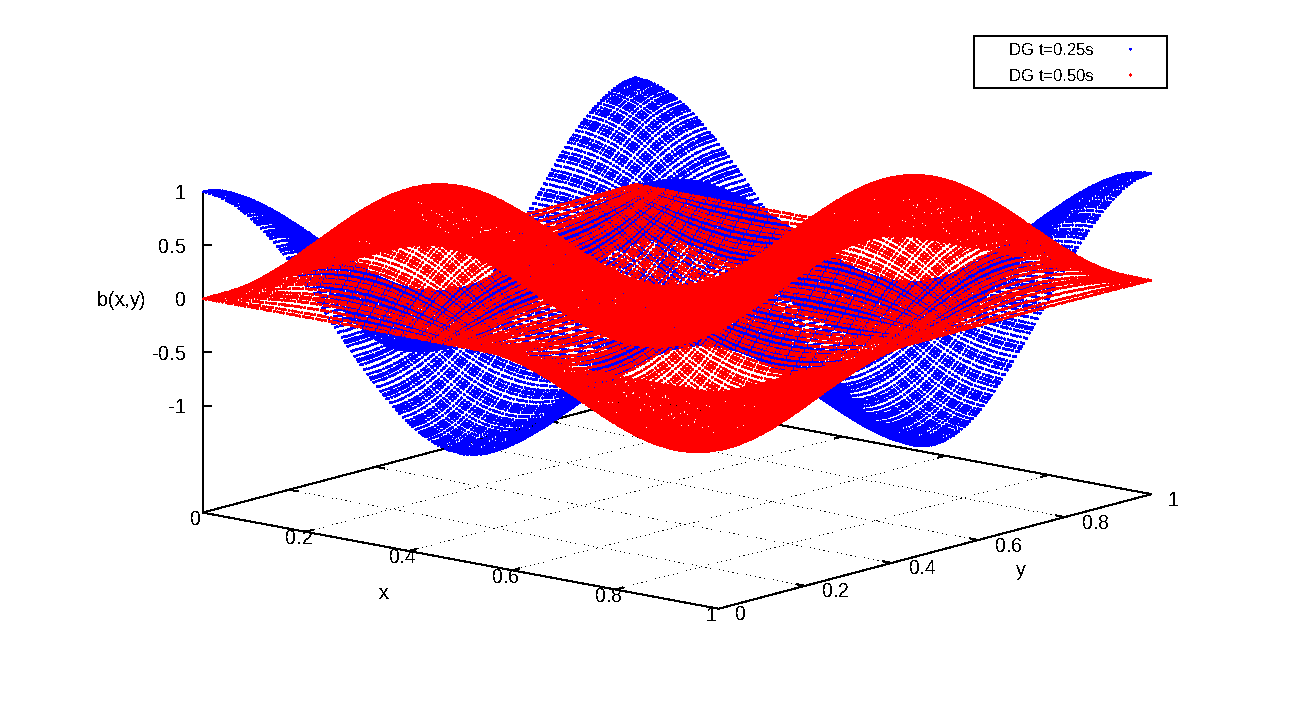
\includegraphics[width=\linewidth]{PNG/Manufacturee/grass_n_x_40_2D.pdf}
        \caption{Vue d'ensemble}
        \label{fig:grass_2d_global}
    \end{subfigure}
    
    \vspace{0.4cm} % Petit espacement vertical entre les deux images
    
    % --- Seconde sous-figure (Vue de tranche / coupe) ---
    \begin{subfigure}{0.96\linewidth}
        \centering
        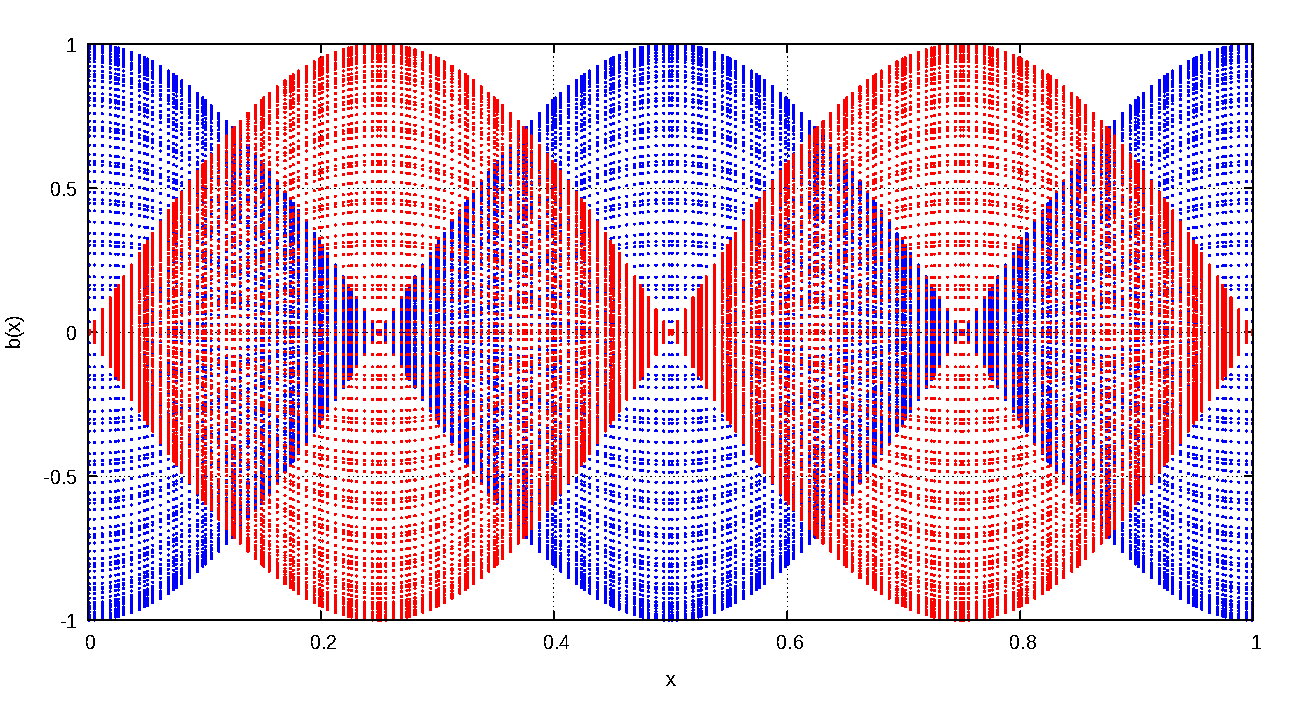
\includegraphics[width=0.9\linewidth]{PNG/Manufacturee/grass_n_x_40_2D_tranche.pdf} % Remplacez par le nom du fichier de profil/tranche
        \caption{Vue de coupe}
        \label{fig:grass_2d_coupe}
    \end{subfigure}
    
    \caption{Cas test 1 -- Représentation des solutions numériques obtenues avec la loi de Grass aux temps $t = \SI{0.25}{\second}$ (en bleu) et $t = \SI{0.5}{\second}$ (en rouge) pour $p = 2$ et $N_e = 40^2$}
    \label{fig:Representation_manufacturee_2D}
\end{figure}

D'un point de vue qualitatif, les figures ci-dessus nous donnent bien le comportement attendu pour $\widetilde{b}$. \\
En effet, sur la figure \ref{fig:grass_2d_global} nous observons que la solution numérique varie entre $[-1, 1]$, qu'elle est positive sur $[0, 0.5] \times [0, 0.5] \cup  [0.5, 1] \times [0.5, 1]$ et négative sur $[0.5, 1] \times [0, 0.5] \cup  [0, 0.5] \times [0.5, 1]$. \\
De plus, sur la figure \ref{fig:grass_2d_coupe}, nous remarquons que la solution effectue une demi-période et une période aux temps $t = \SI{0.25}{\second}$ et $t = \SI{0.5}{\second}$ respectivement.

D'un point de vue quantitatif, le tableau \ref{tab:manufacturee_2D_cartesien} recense les erreurs en norme $L^2$ et $L^\infty$ pour les trois lois empiriques. Nous obtenons bien l'ordre de convergence théorique $p+1 = 3$, validant ainsi notre implémentation pour ce cas test.

\begin{table}[h!]
    \centering
    \small % Réduit légèrement la taille de la police pour s'assurer que le tableau tient dans la page
    \begin{tabular}{r ccc ccc ccc}
    \toprule
    & \multicolumn{3}{c}{\textbf{Loi de Grass}} & \multicolumn{3}{c}{\textbf{Loi de MPM}} & \multicolumn{3}{c}{\textbf{Loi de Van Rijn}} \\
    \cmidrule(lr){2-4} \cmidrule(lr){5-7} \cmidrule(lr){8-10}
    $N_e$ & $L^2$ & $L^\infty$ & Ordre & $L^2$ & $L^\infty$ & Ordre & $L^2$ & $L^\infty$ & Ordre \\
    \midrule
    $20^2$ & 7.62E-05 & 4.09E-04 & -- & 7.71E-05 & 4.24E-04 & -- & 7.71E-05 & 4.29E-04 & -- \\
    $40^2$ & 8.74E-06 & 2.09E-05 & 3.12 & 8.78E-06 & 2.13E-05 & 3.15 & 8.77E-06 & 2.17E-05 & 3.16 \\
    $80^2$ & 1.08E-06 & 2.53E-06 & 3.02 & 1.08E-06 & 2.09E-06 & 3.02 & 1.08E-06 & 2.10E-06 & 3.02 \\
    $160^2$ & 1.35E-07 & 3.25E-07 & 3.00 & 1.35E-07 & 2.58E-07 & 3.00 & 1.35E-07 & 2.59E-07 & 3.00 \\
    \bottomrule
    \end{tabular}
    \caption{Cas test 1 -- Erreurs d'approximation en norme $L^2$, $L^\infty$ au temps $t = \SI{0.5}{\second}$ et ordres de convergence associés pour les lois de Grass, MPM et Van Rijn pour $p = 2$}
    \label{tab:manufacturee_2D_cartesien}
\end{table}

\subsection{Cas test 2 : Solution manufacturée 1D}

L'enjeu de ce cas test est de vérifier que nous retrouvons les résultats obtenus avec le code 1D en imposant des conditions périodiques sur les bords Nord et Sud du domaine. \\
Pour rappel, on impose la solution manufacturée
\begin{equation}
    \begin{aligned}
        & \widetilde{b}(\bm{x}, t) = \sin \left( 2 \pi (x - t) \right) \\
        & \bm{\widetilde{u}}(\bm{x}, t) = \left( 1 + \frac{1}{2} \widetilde{b}(\bm{x}, t) \right) e_x \\
        & \widetilde{h}(\bm{x}, t) = \frac{\widetilde{q}}{\| \bm{\widetilde{u}}(\bm{x}, t) \|}
    \end{aligned}
\end{equation}
où $\widetilde{q}$ est un flux constant et la simulation est effectuée pour une durée d'une période.

\begin{figure}[h!]
    \centering
    % --- Première sous-figure (Vue principale) ---
    \centering
    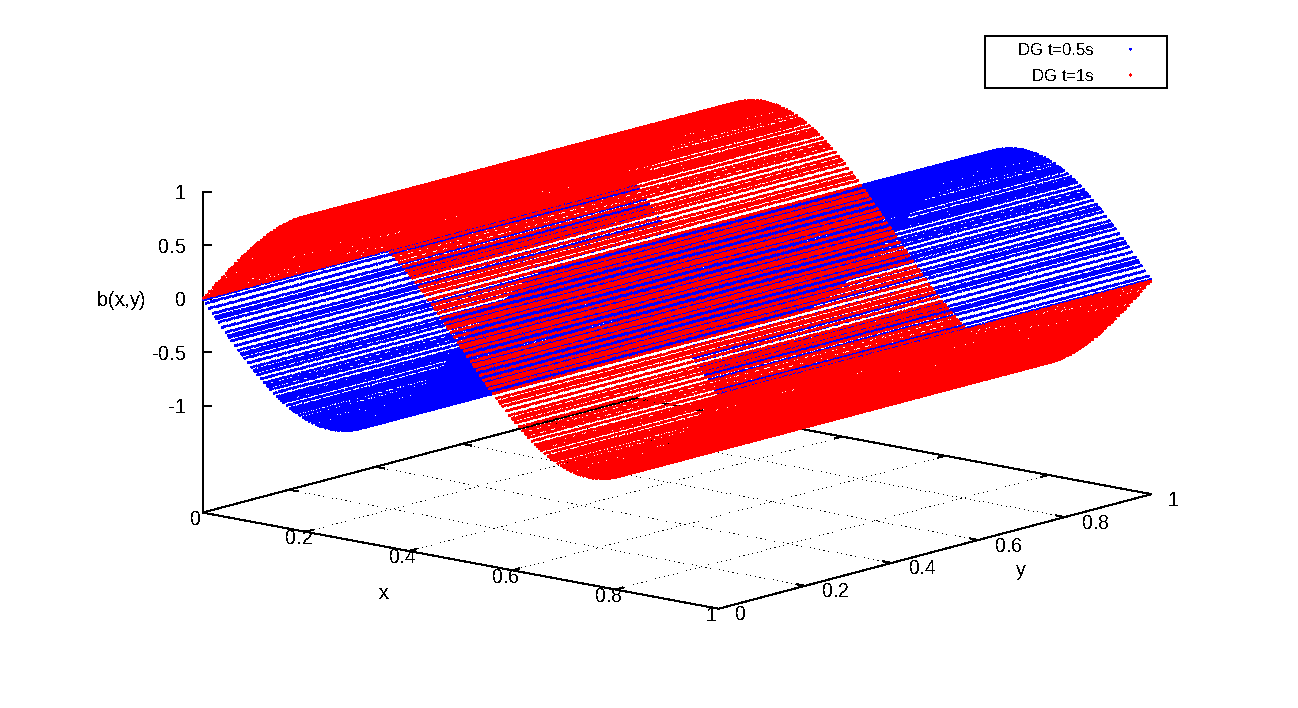
\includegraphics[width=\linewidth]{PNG/Manufacturee/mpm_n_x_40_1D.pdf}
    \caption{Cas test 2 -- Représentation des solutions numériques obtenues avec la loi de MPM aux temps $t = \SI{0.5}{\second}$ (en bleu) et $t = \SI{1}{\second}$ (en rouge) pour $p = 2$ et $N_e = 40^2$}
    \label{fig:Representation_manufacturee_1D}
\end{figure}

Qualitativement, sur la figure \ref{fig:Representation_manufacturee_1D}, nous reconnaissons bien une translation purement 1D de la bathymétrie imposée par la soluton manufacturée. \\
Quantitativement, une étude de l'ordre de convergence pour les trois lois est présentée dans le tableau \ref{tab:manufacturee_1D_cartesien} et nous obtenons l'ordre de convergence théorique, validant donc l'aptitude de notre modèle 2D à traiter des problèmes 1D dans le cas d'une solution manufacturée.

\begin{table}[h!]
    \centering
    \small % Réduit légèrement la taille de la police pour s'assurer que le tableau tient dans la page
    \begin{tabular}{r ccc ccc ccc}
    \toprule
    & \multicolumn{3}{c}{\textbf{Loi de Grass}} & \multicolumn{3}{c}{\textbf{Loi de MPM}} & \multicolumn{3}{c}{\textbf{Loi de Van Rijn}} \\
    \cmidrule(lr){2-4} \cmidrule(lr){5-7} \cmidrule(lr){8-10}
    $N_e$ & $L^2$ & $L^\infty$ & Ordre & $L^2$ & $L^\infty$ & Ordre & $L^2$ & $L^\infty$ & Ordre \\
    \midrule
    $20^2$ & 7.12E-05 & 1.57E-04 & -- & 7.13E-05 & 1.49E-04 & -- & 7.14E-05 & 1.51E-04 & -- \\
    $40^2$ & 8.68E-06 & 1.73E-05 & 3.03 & 8.71E-06 & 1.75E-05 & 3.03 & 8.72E-06 & 1.76E-05 & 3.03 \\
    $80^2$ & 1.08E-06 & 2.10E-06 & 3.00 & 1.08E-06 & 2.09E-06 & 3.00 & 1.08E-06 & 2.10E-06 & 3.00 \\
    $160^2$ & 1.35E-07 & 2.62E-07 & 3.00 & 1.35E-07 & 2.58E-07 & 3.00 & 1.35E-07 & 2.59E-07 & 3.00 \\
    \bottomrule
    \end{tabular}
    \caption{Cas test 2 -- Erreurs d'approximation en norme $L^2$, $L^\infty$ au temps $t = \SI{1}{\second}$ et ordres de convergence associés pour les lois de Grass, MPM et Van Rijn pour $p = 2$}
    \label{tab:manufacturee_1D_cartesien}
\end{table}

\subsection{Cas test 3 : Solution analytique de Berthon \textit{et al.}}

\enlargethispage{2\baselineskip}

L'objectif de ce dernier cas test est de vérifier que notre schéma numérique fonctionne comme attendu sur une solution analytique non-manufacturée. \\
De même qu'en 1D, les constantes de la solution de Berthon \textit{et al.} \cite{berthon2012analytical} sont fixées de telle sorte à ce que le résultat numérique soit identique pour les trois lois empiriques caractérisant le flux $\bm{G}$. \\
En outre, nous imposons des conditions de Neumann homogène sur les bords Nord et Sud du domaine, permettant ainsi de retrouver un écoulement 1D. \\
Qualitativement, comme quantitativement, nous obtenons les résultats attendus, finalisant la validation de notre solveur 2D.

\begin{figure}[h!]
    \centering
    % --- Première sous-figure (Vue principale) ---
    \centering
    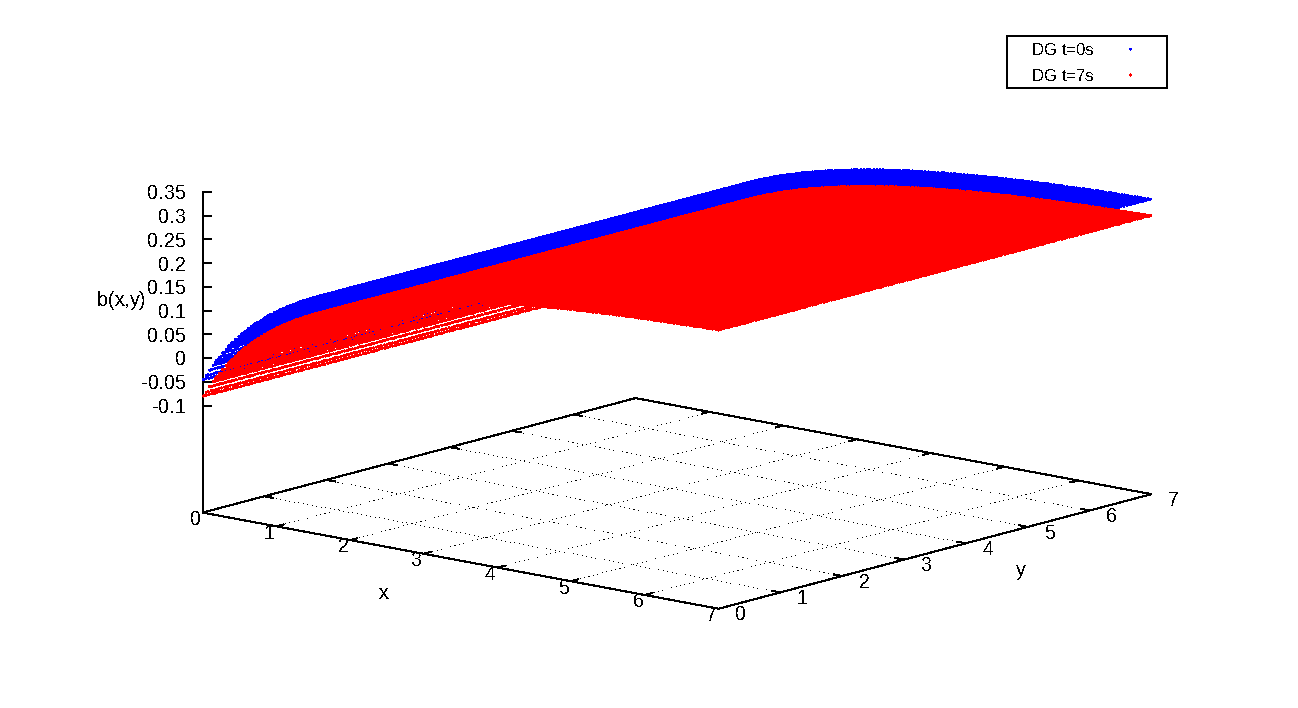
\includegraphics[width=\linewidth]{PNG/Berthon/vr_n_x_40_2D.pdf}
    \caption{Cas test 3 -- Représentation des solutions numériques obtenues avec la loi de Van Rijn aux temps $t = \SI{0}{\second}$ (en bleu) et $t = \SI{7}{\second}$ (en rouge) pour $p = 2$ et $N_e = 40^2$}
    \label{fig:Representation_berthon_1D}
\end{figure}

\begin{table}[h!]
    \centering
    \small % Réduit légèrement la taille de la police pour s'assurer que le tableau tient dans la page
    \begin{tabular}{r ccc ccc ccc}
    \toprule
    & \multicolumn{3}{c}{\textbf{Loi de Grass}} & \multicolumn{3}{c}{\textbf{Loi de MPM}} & \multicolumn{3}{c}{\textbf{Loi de Van Rijn}} \\
    \cmidrule(lr){2-4} \cmidrule(lr){5-7} \cmidrule(lr){8-10}
    $N_e$ & $L^2$ & $L^\infty$ & Ordre & $L^2$ & $L^\infty$ & Ordre & $L^2$ & $L^\infty$ & Ordre \\
    \midrule
    $10^2$ & 9.81E-04 & 6.01E-04 & -- & 9.62E-04 & 5.89E-04 & -- & 9.62E-04 & 5.89E-04 & -- \\
    $20^2$ & 1.42E-04 & 1.12E-04 & 2.78 & 1.39E-04 & 1.09E-04 & 2.78 & 1.39E-04 & 1.10E-04 & 2.78 \\
    $40^2$ & 1.87E-05 & 1.76E-05 & 2.92 & 1.83E-05 & 1.73E-05 & 2.92 & 1.83E-05 & 1.72E-05 & 2.92 \\
    $80^2$ & 2.37E-06 & 2.50E-06 & 2.98 & 2.32E-06 & 2.44E-06 & 2.98 & 2.32E-06 & 2.44E-06 & 2.98 \\
    \bottomrule
    \end{tabular}
    \caption{Cas test 3 -- Erreurs d'approximation en norme $L^2$, $L^\infty$ au temps $t = \SI{7}{\second}$ et ordres de convergence associés pour les lois de Grass, MPM et Van Rijn pour $p = 2$}
    \label{tab:convergence_berthon}
\end{table}

\chapter{Système d'équations de Saint-Venant-Exner et formulation de Galerkin discontinue}

Dans ce dernier chapitre, nous allons établir un schéma RKDG pour le système \eqref{eq:Saint_Venant_Exner}, puis nous validerons notre implémentation sur des cas tests de référence.

\section{Système de Saint-Venant-Exner}

Soit $\Omega$ un ouvert convexe de $\mathbb{R}^2$. Le système d'équations de Saint-Venant sous forme conservative s'écrit :
\begin{equation} \tag{$\mathcal{SW}$} \label{eq:Saint_Venant} 
    \left \{
    \begin{aligned}
        & \partial_t h + \nabla \cdot \left( h \bm{u} \right) = 0 && \text{sur } \Omega \times (0, T) \\
        & \partial_t (h \bm{u}) + \nabla \cdot \left( h \bm{u} \otimes \bm{u} + g \frac{h^2}{2} \mathbb{I} \right) = - g h \nabla b && \text{sur } \Omega \times (0, T) \\
        & h(\bm{x}, t) = h_D(\bm{x}, t) \text{ et } \bm{u}(\bm{x}, t) = \bm{u}_D(\bm{x}, t) && \text{sur } \Gamma_D \times (0, T) \\
        & \mathbb{G}_\text{SW}(h, \bm{u}) \cdot \bm{n} = \bm{g}_N(\bm{x}, t) && \text{sur } \Gamma_N \times (0, T) \\
        & h(\bm{x}, 0) = h_\text{ini}(\bm{x}) \text{ et } \bm{u}(\bm{x}, 0) = \bm{u}_\text{ini}(\bm{x}) && \text{sur } \Omega
    \end{aligned}
    \right .
\end{equation} 
où $\mathbb{I}$ est la matrice identité, $h(\bm{x}, t) : \Omega \times (0, T) \longrightarrow \mathbb{R}$ est la hauteur d'eau, $\bm{u}(\bm{x}, t) : \Omega \times (0, T) \longrightarrow \mathbb{R}^2$ est la vitesse horizontale et $\mathbb{G}_\text{SW}$ est le tenseur des flux de Saint-Venant défini par
\begin{equation}
    \mathbb{G}_\text{SW}(h, \bm{u}) = \begin{pmatrix}
        hu & hv \\
        hu^2 + g \frac{h^2}{2} & huv \\
        huv & hv^2 + g \frac{h^2}{2}
    \end{pmatrix}
\end{equation}
En outre, l'évolution de la bathymétrie est régie par l'équation d'Exner \eqref{eq:Exner_generalisee}, ce qui nous conduit au système couplé de Saint-Venant-Exner :
\begin{equation} \tag{$\mathcal{SWE}$} \label{eq:Saint_Venant_Exner}
    \left \{
    \begin{aligned}
        & \partial_t h + \nabla \cdot \left( h \bm{u} \right) = 0 && \text{sur } \Omega \times (0, T) \\
        & \partial_t (h \bm{u}) + \nabla \cdot \left( h \bm{u} \otimes \bm{u} + g \frac{h^2}{2} \mathbb{I} \right) = - g h \nabla b && \text{sur } \Omega \times (0, T) \\
        & m(\nabla b) \partial_t b + \nabla \cdot \bm{G} = S && \text{sur } \Omega \times (0, T) \\
        & + \text{Conditions aux limites} \\
        & + \text{Conditions initiales}
    \end{aligned}
    \right .
\end{equation}

L'étude des valeurs propres de \eqref{eq:Saint_Venant_Exner} est primordiale car, d'une part, elles permettent de déterminer le domaine d'hyperbolicité du système et, d'autre part, elles sont utilisées pour définir la diffusion numérique des flux de Rusanov. \\
Ainsi, en introduisant le débit hydraulique $\bm{q} = (q_x, q_y) = h \bm{u} = (hu, hv)$, le système de Saint-Venant-Exner sous forme quasi-conservative s'écrit :
\begin{equation}
    \left \{
    \begin{aligned}
        & \partial_t h + \partial_x q_x + \partial_y q_y = 0 \\
        & \partial_t q_x + \partial_x \left( \frac{q_x^2}{h} + g \frac{h^2}{2} \right) + \partial_y \left( \frac{q_x q_y}{h} \right) = - g h \partial_x b \\
        & \partial_t q_y + \partial_x \left( \frac{q_x q_y}{h} \right) + \partial_y \left( \frac{q_y^2}{h} + g \frac{h^2}{2} \right) = - g h \partial_y b \\
        & m(\nabla b) \partial_t b + \partial_x G_x + \partial_y G_y = S
    \end{aligned}
    \right .
\end{equation}
où $G_x$ et $G_y$ sont les composantes suivant $x$ et $y$ du flux sédimentaire $\bm{G}$. \\
Ce système d'équations peut se réécrire sous la forme matricielle
\begin{equation}
    \mathbb{M}(\nabla b) \partial_t \bm{W} + \nabla \cdot \mathbb{G}(\bm{W}) = \bm{S}(\bm{W})
\end{equation}
où $\bm{W} = (h, q_x, q_y, b)^T$ désigne le vecteur des variables d'état, $\mathbb{M}(\nabla b) = \text{diag}(1, 1, 1, m(\nabla b))$ est la matrice liée à la métrique géométrique et $\mathbb{G}(\bm{W}) = (\bm{G}_1(\bm{W}), \bm{G}_2(\bm{W}))$ est le tenseur des flux physiques conservatifs avec
\begin{equation}
    \bm{G}_1(\bm{W}) = \begin{pmatrix}
        q_x \\
        \frac{q_x^2}{h} + g \frac{h^2}{2} \\
        \frac{q_x q_y}{h} \\
        G_x
    \end{pmatrix}, \quad
    \bm{G}_2(\bm{W}) = \begin{pmatrix}
        q_y \\
        \frac{q_y^2}{h} + g \frac{h^2}{2} \\
        \frac{q_y q_x}{h} \\
        G_y
    \end{pmatrix}, \quad
    \bm{S}(\bm{W}) = \begin{pmatrix}
        0 \\
        - gh \partial_x b \\
        - gh \partial_y b \\
        S
    \end{pmatrix}
\end{equation}
Afin de pouvoir mener l'étude spectrale, il est nécessaire de passer à la forme quasi-linéaire
\begin{equation}
    \partial_t \bm{W} + \mathbb{J}_1(\bm{W}) \partial_x \bm{W} + \mathbb{J}_2(\bm{W}) \partial_y \bm{W} = \bm{S}_\text{ext}(\bm{W})
\end{equation}
avec $\bm{S}_\text{ext}(\bm{W}) = (0, 0, 0, S/m(\nabla b))^T$ le vecteur de termes sources externes (lié aux caractéristiques du lit sédimentaire) et
\begin{equation}
    \begin{aligned}
        \mathbb{J}_1(\bm{W}) & = \mathbb{M}^{-1}(\nabla b) \frac{\partial \bm{G}_1(\bm{W})}{\partial \bm{W}} + \begin{pmatrix}
            0 & 0 & 0 & 0 \\
            0 & 0 & 0 & gh \\
            0 & 0 & 0 & 0 \\
            0 & 0 & 0 & 0 \\
        \end{pmatrix}
        = \begin{pmatrix}
            0 & 1 & 0 & 0 \\
            gh - u^2 & 2u & 0 & gh \\
            -uv & v & u & 0 \\
            \alpha_x & \beta_x & \gamma_x & 0
        \end{pmatrix} \\
        \mathbb{J}_2(\bm{W}) & = \mathbb{M}^{-1}(\nabla b) \frac{\partial \bm{G}_2(\bm{W})}{\partial \bm{W}} + \begin{pmatrix}
            0 & 0 & 0 & 0 \\
            0 & 0 & 0 & 0 \\
            0 & 0 & 0 & gh \\
            0 & 0 & 0 & 0 \\
        \end{pmatrix}
        = \begin{pmatrix}
            0 & 0 & 1 & 0 \\
            - uv & v & u & 0 \\
            gh - v^2 & 0 & 2v & gh \\
            \alpha_y & \beta_y & \gamma_y & 0
        \end{pmatrix}
    \end{aligned}
\end{equation}
où, similairement pour $x$ et $y$,
\begin{equation}
    \alpha_x = \frac{1}{m(\nabla b)} \frac{\partial G_x}{\partial h}, \quad \beta_x = \frac{1}{m(\nabla b)} \frac{\partial G_x}{\partial q_x}, \quad \gamma_x = \frac{1}{m(\nabla b)} \frac{\partial G_x}{\partial q_y}
\end{equation}
Pour que le système \eqref{eq:Saint_Venant_Exner} soit strictement hyperbolique, il est nécessaire que les valeurs propres de
\begin{equation}
    \mathbb{H}(\bm{W}) = \mathbb{J}_1 n_x + \mathbb{J}_2 n_y = \begin{pmatrix}
        0 & n_x & n_y & 0 \\
        (gh - u^2) n_x - uv n_y & 2u n_x + v n_y & u n_y & gh n_x \\
        (gh - v^2) n_y - uv n_x & v n_x & 2v n_y + u n_x & gh n_y \\
        \alpha_n & \beta_n & \gamma_n & 0
    \end{pmatrix}
\end{equation}
soient réelles et distinctes selon toute direction $\bm{n} = (n_x, n_y)$ avec $\bm{n}$ une normale unitaire et
\begin{equation}
    \alpha_n = \alpha_x n_x + \alpha_y n_y, \quad \beta_n = \beta_x n_x + \beta_y n_y, \quad \gamma_n = \gamma_x n_x + \gamma_y n_y
\end{equation}

Le développement en Annexe \ref{annexe:polynome_caracteristique} nous conduit au polynôme caractéristique de $\mathbb{H}$ suivant :
\begin{equation}
    \begin{aligned}
        \chi_H(\lambda) & = \lambda^4 - 3u_n \lambda^3 + \left[ 3 u_n^2 -gh(1 + \beta_n n_x + \gamma_n n_y) \right] \lambda^2 \\
        & - \left[ u_n(u_n^2 - gh) + gh \left( \alpha_n - u_n(\beta_n n_x + \gamma_n n_y) + (u n_y - v n_x)(\beta_n n_y - \gamma_n n_x) \right) \right] \lambda \\
        & + gh u_n \left[ \alpha_n + (\beta_n n_y - \gamma_n n_x)(u n_y - v n_x) \right]
    \end{aligned}
\end{equation}
où nous avons posé $u_n = u n_x + v n_y$ la composante normale de la vitesse. \\
En outre, si on introduit $u_t = u n_y - v n_x$ la composante tangentielle de la vitesse, $\delta_n = \beta_n n_x + \gamma_n n_y$ et $\delta_t = \beta_n n_y - \gamma_n n_x$ les sensibilités du flux sédimentaire aux variations de débit normal et tangentiel respectivement, $\chi_H$ peut s'écrire
\begin{equation}
    \begin{aligned}
        \chi_H(\lambda) & = \lambda^4 - 3u_n \lambda^3 + \left[ 3 u_n^2 -gh(1 + \delta_n) \right] \lambda^2 \\
        & - \left[ u_n(u_n^2 - gh) + gh \left( \alpha_n - u_n \delta_n + u_t \delta_t \right) \right] \lambda + gh u_n \left[ \alpha_n + u_t \delta_t \right]
    \end{aligned}
\end{equation}
ce qui conduit à la forme
\begin{equation} \label{eq:Polynome_caracteristique}
    \chi_H = \lambda(\lambda - u_n) \left[ (\lambda - u_n)^2 - gh \right] - gh \left[ \delta_n \lambda^2 + \left( \alpha_n - u_n \delta_n + u_t \delta_t \right) \lambda - u_n \left( \alpha_n + u_t \delta_t \right) \right]
\end{equation}
Cette dernière écriture met en avant l'impact de l'équation d'Exner sur les valeurs propres usuelles du système de Saint-Venant. \\
En effet, si nous considérons un fond fixe, alors $\alpha_n = \delta_n = \delta_t = 0$ donc :
\begin{equation}
    \chi_H(\lambda) = \lambda(\lambda - u_n) \left[ (\lambda - u_n)^2 - gh \right] = \lambda (\lambda - u_n) \left( \lambda - \left[u_n - \sqrt{gh}\right] \right) \left( \lambda - \left[ u_n + \sqrt{gh} \right] \right)
\end{equation}
Nous reconnaissons ainsi les trois valeurs propres usuelles de Saint-Venant, ainsi qu'une quatrième valeur propre nulle liée à la bathymétrie fixe. \\
Par conséquent, l'équation d'Exner agit comme une perturbation de la vitesse des ondes du système de Saint-Venant. \\

De plus, le polynôme caractéristique \eqref{eq:Polynome_caracteristique} nous permet de retrouver la valeur propre de De Vries en 1D et d'étendre cette dernière en 2D. \\
Pour ce faire, comme l'échelle de temps de l'évolution de la bathymétrie est lente devant la dynamique de l'eau en régime sous-critique, l'idée de De Vries \cite{vries1965considerations} est d'effectuer un développement limité à l'ordre 1 autour de $\lambda = 0$. \\
Ainsi, il vient
\begin{equation}
    - \left[ u_n(u_n^2 - gh) + gh \left( \alpha_n - u_n \delta_n + u_t \delta_t \right) \right] \lambda_\text{DV} + gh u_n \left[ \alpha_n + u_t \delta_t \right] = 0
\end{equation}
soit
\begin{equation}
    \lambda_\text{DV} = \frac{\left( \alpha_n + u_t \delta_t \right) u_n}{-u_n \left( 1 - \text{Fr}_n^2 \right) + \alpha_n + u_t \delta_t - u_n \delta_n}
\end{equation}
En particulier, si nous utilisons la loi de Grass en 2D, alors
\begin{equation}
    \begin{aligned}
        G_n & = A_G \frac{1}{h^{m_G}} \| \bm{q} \|^{m_G - 1} q_n \\
        \alpha_n & = -m_G A_G \frac{1}{h^{m_G + 1}} \| \bm{q} \| q_n = - m_G \frac{1}{h} G_n \\
        \beta_n & = A_G \frac{1}{h} \| \bm{u} \|^{m_G - 1} \left( n_x + (m_G - 1) \frac{u}{\| \bm{u} \|^2} u_n \right) \\
        \gamma_n & = A_G \frac{1}{h} \| \bm{u} \|^{m_G - 1} \left( n_y + (m_G - 1) \frac{v}{\| \bm{u} \|^2} u_n \right) \\
    \end{aligned}
\end{equation}
D'où
\begin{equation}
    \begin{aligned}
        \delta_n & = A_G \frac{1}{h} \| \bm{u} \|^{m_G - 1} \left( 1 + (m_G - 1) \frac{u_n^2}{\| \bm{u} \|^2} \right) = \frac{G_n}{h u_n} \left( 1 + (m_G - 1) \frac{u_n^2}{\| \bm{u} \|^2} \right) \\
        \delta_t & = A_G \frac{1}{h} \| \bm{u} \|^{m_G - 1} (m_G - 1) \frac{u_t}{\| \bm{u} \|^2} u_n = \frac{G_n}{h u_n} (m_G - 1) \frac{u_n u_t}{\| \bm{u} \|^2}
    \end{aligned}
\end{equation}
Par conséquent,
\begin{equation}
    \alpha_n + u_t \delta_t = - u_n \delta_n
\end{equation}
On obtient alors la valeur propre de De Vries en 2D pour la loi de Grass sous la forme
\begin{equation}
    \lambda_\text{DV} = \frac{\delta_n}{1 - \text{Fr}_n^2 + 2 \delta_n} u_n
\end{equation}
En outre, pour un écoulement 1D, $\delta_n = \beta_n = \beta$ et $u_n = u$, d'où
\begin{equation}
    \lambda_\text{DV,1D} = \frac{\beta}{1 - \text{Fr}^2 + 2 \beta} u
\end{equation}
Or, comme le flux de sédiments $G$ est petit devant le débit d'eau $q$ lorsque l'écoulement est en régime sous-critique et que
\begin{equation}
    \beta \sim m_G \frac{G}{q} \ll 1 - \text{Fr}^2
\end{equation}
nous retrouvons la valeur propre de De Vries en 1D pour la loi de Grass \cite{fernandez2025third, vries1965considerations}
\begin{equation}
    \lambda_\text{DV,1D} = \frac{\beta}{1 - \text{Fr}^2} u
\end{equation}
Enfin, comme chaque terme de perturbation hydro-sédimentaire du polynôme caractéristique $\chi_H$ est proportionnel au ratio $G_n/q_n$, nous pouvons en première approximation conserver les trois autres valeurs propres usuelles issues de \eqref{eq:Saint_Venant}. \\
Autrement, si nous souhaitions trouver les racines exactes, il faudrait effectuer une méthode itérative pour chaque face à chaque sous-pas de temps. Ce processus est très coûteux d'une part, et rien ne garantit que la méthode converge vers les vraies racines d'autre part. \\
Cependant, Fernandez-Nieto \textit{et al.} \cite{fernandez2025third} ont montré que les approximations de De Vries ne sont valables que pour des nombres de Froude inférieurs à $0.7$ environ. Au-delà, les valeurs propres sont sur-estimées, entraînant une sur-diffusion numérique. En ce sens, il serait possible d'implémenter une méthode itérative dès lors que le nombre de Froude local $\text{Fr}_n > 0.7$.

\section{Formulation semi-discrète}

La résolution du système \eqref{eq:Saint_Venant_Exner} s'appuie sur une approche par couplage faible, en le scindant en deux sous-problèmes \eqref{eq:Saint_Venant} + \eqref{eq:Exner_generalisee}. À chaque sous-pas du schéma temporel, chaque sous-système est résolu séquentiellement en gelant le vecteur d'état de l'autre. \\
D'une part, la discrétisation des équations de Saint-Venant par un schéma RKDG a fait l'objet de la thèse de Camille Poussel \cite{poussel2024dynamique} ; nous réutiliserons donc directement ses formulations \textit{well-balanced} semi-discrètes et discrètes. D'autre part, nous avons établi dans ce travail la formulation RKDG de l'équation d'Exner. Ainsi, il ne reste plus qu'à assembler ces deux formulations pour obtenir le schéma RKDG complet du système Saint-Venant-Exner. \\

On se donne un maillage conforme et non uniforme $\mathcal{M}^n$ du domaine physique $\Omega \subset \mathbb{R}^2$ au temps $t^n$. \\
Le problème variationnel semi-discret DG pour les équations de Saint-Venant s'écrit
\begin{equation} \tag{$\mathcal{P}_{SD}^\mathcal{SW}$} \label{eq:Probleme_variationnel_Saint_Venant}
    \left \{
    \begin{aligned}
        & \text{Trouver } \bm{W}_h \in \left[ \mathcal{V}^\mathbf{p}(\mathcal{M}^n) \right]^3 \text{ tel que } \forall \bm{\varphi} \in \left[ \mathcal{V}^\mathbf{p}(\mathcal{M}^n) \right]^3 \\
        & m_\mathcal{SW}^n(\partial_t \bm{W}_h, \bm{\varphi}) + a_\mathcal{SW}^n(\bm{\varphi}; \bm{W}_h, b_h) = l_\mathcal{SW}^n(\bm{\varphi})
    \end{aligned}
    \right .
\end{equation}
où les applications DG $m_\mathcal{SW}^n$ et $a_\mathcal{SW}^n$, et la forme linéaire $l_\mathcal{SW}^n$ sont définies comme
\begin{equation}
    \begin{aligned}
        \forall \bm{v}, \bm{\varphi} \in \left[ \mathcal{V}^\mathbf{p}(\mathcal{M}^n) \right]^3, ~
        & m_\mathcal{SW}^n(\bm{v}, \bm{\varphi}) = \sum_{\Omega_i^n \in \mathcal{M}^n} \int_{\Omega_i^n} \bm{v} \cdot \bm{\varphi} \text{d}\bm{x} \\
        & a_\mathcal{SW}^n(\bm{\varphi}; \bm{v}, b_h) = - \sum_{\Omega_i^n \in \mathcal{M}^n} \int_{\Omega_i^n} \mathbb{G}_\text{SW}(\bm{v}) : \nabla \bm{\varphi} \text{d}\bm{x} \\
        & \phantom{a_\mathcal{SW}^n(\bm{\varphi}; \bm{v}, b_h) = } - \sum_{F \in \mathcal{F}^\text{int}} \int_F \left( \widehat{\mathbb{G}}_F^\text{wb}(\bm{v}) \cdot \bm{n}_F \right) \cdot \llbracket \bm{\varphi} \rrbracket \text{d}F \\
        & \phantom{a_\mathcal{SW}^n(\bm{\varphi}; \bm{v}, b_h) = } - \sum_{\Omega_i^n \in \mathcal{M}^n} \int_{\Omega_i^n} \bm{S}_\text{SW}(\bm{v}, b_h) \cdot \bm{\varphi} \text{d}\bm{x} \\
        & l_\mathcal{SW}^n(\bm{\varphi}) = - \sum_{F \in \mathcal{F}_D^\partial} \int_F \left( \widehat{\mathbb{G}}_F^\text{wb}(\bm{W}_D) \cdot \bm{n}_F \right) \cdot \bm{\varphi} \text{d}F - \sum_{F \in \mathcal{F}_N^\partial} \int_F \bm{g}_N \cdot \bm{\varphi} \text{d}F
    \end{aligned}
\end{equation}
avec $\displaystyle \widehat{\mathbb{G}}_F^\text{wb}(\bm{W}, b_h) \cdot \bm{n}_F = \widehat{\mathbb{G}}_F \left( \bm{W}^* \right) \cdot \bm{n}_F - \delta_F \left( \bm{W}, b_h \right)$ où $\widehat{\mathbb{G}}_F$ est le flux numérique de Rusanov pour les équations de Saint-Venant. \\
De plus, $\bm{W}^* = (h^*, \bm{q}^*)$ est le vecteur des grandeurs conservatives modifiées de sorte que pour une face $F \in \mathcal{F}^\text{int}$ reliant la maille $\Omega_i^n$ et la maille $\Omega_r^n$,
\begin{equation}
    \begin{aligned}
        & \restricdynamic{h^*}{\Omega_i^n} = \max \left( 0, \restricdynamic{h}{\Omega_i^n} - \max \left( \restricdynamic{b_h}{\Omega_r^n} - \restricdynamic{b_h}{\Omega_i^n}, 0 \right) \right), \quad
        \restricdynamic{\bm{q}^*}{\Omega_i^n} = \restricdynamic{h^*}{\Omega_i^n} \frac{\restricdynamic{\bm{q}}{\Omega_i^n}}{\restricdynamic{h}{\Omega_i^n}} \\
        & \restricdynamic{h^*}{\Omega_r^n} = \max \left( 0, \restricdynamic{h}{\Omega_r^n} - \max \left( \restricdynamic{b_h}{\Omega_i^n} - \restricdynamic{b_h}{\Omega_r^n}, 0 \right) \right), \quad
        \restricdynamic{\bm{q}^*}{\Omega_r^n} = \restricdynamic{h^*}{\Omega_r^n} \frac{\restricdynamic{\bm{q}}{\Omega_r^n}}{\restricdynamic{h}{\Omega_r^n}}
    \end{aligned}
\end{equation}
Enfin, $\delta_F$ est le terme source additionnel rendant le schéma \textit{well-balanced} défini par
\begin{equation}
    \delta_F(\bm{W}, b_h) = \begin{pmatrix}
        0 \\
        \frac{g}{4} \left( \restricdynamic{h^*}{\Omega_i^n}^2 - \restricdynamic{h}{\Omega_i^n}^2 + \restricdynamic{h^*}{\Omega_r^n}^2 - \restricdynamic{h}{\Omega_r^n}^2 \right) n_{F, x} \\
        \frac{g}{4} \left( \restricdynamic{h^*}{\Omega_i^n}^2 - \restricdynamic{h}{\Omega_i^n}^2 + \restricdynamic{h^*}{\Omega_r^n}^2 - \restricdynamic{h}{\Omega_r^n}^2 \right) n_{F, y}
    \end{pmatrix}
\end{equation}
et $\bm{S}_\text{SW}$ reste le vecteur terme source usuel de \eqref{eq:Saint_Venant}
\begin{equation}
    \bm{S}_\text{SW}(\bm{W}, b_h) = \begin{pmatrix}
        0 \\
        - gh \partial_x b_h \\
        - gh \partial_y b_h
    \end{pmatrix}
\end{equation}

La formulation variationnelle \eqref{eq:Probleme_variationnel_Saint_Venant} peut se réécrire sous la forme matricielle locale
\begin{equation} \tag{$\mathcal{P}_M^\mathcal{SW}$} \label{eq:Probleme_matriciel_Saint_Venant}
    \left \{
    \begin{aligned}
        & \forall i \in \llbracket 1, N_e \rrbracket, \text{ trouver } \bm{W}_i \in \mathbb{R}^{3N_\text{ddl}^i} \text{ tel que} \\
        & \mathbb{M}_i \partial_t \bm{W}_i(t) = \bm{\mathcal{I}}_i^{EF}(t) - \bm{\mathcal{I}}_i^{VF}(t) + \bm{\mathcal{I}}_i^S(t) \\
        & \bm{W}_i(0) = \bm{W}_i^0
    \end{aligned}
    \right .
\end{equation}
avec
\begin{itemize}
    \item $\displaystyle \mathbb{M}_i = \int_{\widehat{\Omega}} \mathbb{D}_i(\xi, \eta) \mathbb{D}_i^T(\xi, \eta) \lvert \Omega_i^n \rvert \text{d}\widehat{\Omega} \in \mathbb{R}^{3N_\text{ddl}^i \times 3N_\text{ddl}^i}$ la matrice de masse
    \item $\displaystyle \bm{\mathcal{I}}_i^{EF}(t) = \int_{\widehat{\Omega}} \widetilde{\nabla}_i \mathbb{D}_i(\xi, \eta) : \mathbb{G}_\text{SW}^T \left( \mathbb{D}_i^T(\xi, \eta) \bm{W}_i(t) \right) \lvert \Omega_i^n \rvert \text{d}\widehat{\Omega} \in \mathbb{R}^{3N_\text{ddl}^i}$ le vecteur de contribution volumique du flux
    \item $\displaystyle \bm{\mathcal{I}}_i^{VF}(t) = \sum_{F \in \partial \Omega_i^n} \int_{\widehat{F}} \mathbb{D}_F(\xi) \left( \widehat{\mathbb{G}}_F^\text{wb} \cdot \bm{n}_F \right) \lvert F \rvert \text{d}\widehat{F} \in \mathbb{R}^{3N_\text{ddl}^i}$ le vecteur de contribution du flux aux interfaces
    \item $\displaystyle \bm{\mathcal{I}}_i^S(t) = \int_{\widehat{\Omega}} \mathbb{D}_i(\xi, \eta) \bm{S}_\text{SW} \left( \mathbb{D}_i^T(\xi, \eta) \bm{W}_i(t), \bm{\Phi}_i^T(\xi, \eta) \bm{B}_i(t) \right) \lvert \Omega_i^n \rvert \text{d}\widehat{\Omega} \in \mathbb{R}^{3N_\text{ddl}^i}$ le vecteur de contribution volumique du terme source
\end{itemize}
avec $\mathbb{D}_F(\xi) = \text{diag} \left( \bm{\Phi}_F(\xi), \dots, \bm{\Phi}_F(\xi) \right)$ l'extension à $l$ équations couplées du vecteur $\bm{\Phi}_F \in \mathbb{R}^{N_\text{ddl}^i}$ contenant la base de l'espace polynomial $\mathbb{P}^{p_i}(\Omega_i^n)$ évalué sur la face $F$. \\

Finalement, nous pouvons coupler les deux problèmes matriciels \eqref{eq:Probleme_matriciel_Saint_Venant} et \eqref{eq:Probleme_matriciel_exner} de sorte à obtenir la formulation matricielle semi-discrète DG de \eqref{eq:Saint_Venant_Exner}. Il vient
\begin{equation} \tag{$\mathcal{P}_M^\mathcal{SWE}$}
    \left \{
    \begin{aligned}
        & \forall i \in \llbracket 1, N_e \rrbracket, \text{ trouver } \bm{W}_i \in \mathbb{R}^{3N_\text{ddl}^i} \text{ et } \bm{B}_i \in \mathbb{R}^{N_\text{ddl}^i} \text{ tels que} \\
        & \mathbb{M}_i^\mathcal{SW} \partial_t \bm{W}_i(t) = \bm{\mathcal{I}}_i^{\mathcal{SW}, EF} \left( \bm{W}_i \right) - \bm{\mathcal{I}}_i^{\mathcal{SW}, VF} \left( \bm{W}_i, \bm{B}_i \right) + \bm{\mathcal{I}}_i^{\mathcal{SW}, S} \left( \bm{W}_i, \bm{B}_i \right) \\
        & \mathbb{M}_i^\mathcal{E}(t) \partial_t \bm{B}_i(t) = \bm{\mathcal{I}}_i^{\mathcal{E}, EF} \left( \bm{B}_i, \bm{W}_i , \tau_i \right) - \bm{\mathcal{I}}_i^{\mathcal{E}, VF} \left( \bm{B}, \bm{W}, \bm{\tau} \right) + \bm{\mathcal{I}}_i^{\mathcal{E}, S} \left( \bm{B}_i, \bm{W}_i, \tau_i \right) \\
        & \bm{W}_i(0) = \bm{W}_i^0 \\
        & \bm{B}_i(0) = \bm{B}_i^0
    \end{aligned}
    \right .
\end{equation}
où les annotations $\mathcal{SW}$ et $\mathcal{E}$ font référence aux intégrales définies dans les problèmes matriciels de Saint-Venant et d'Exner respectivement.

\section{Formulation discrète}

La discrétisation temporelle des formulations matricielles semi-discrètes de Saint-Venant et d'Exner s'appuie respectivement sur les schémas SSP(3,3) de Shu-Osher et IMEX-SSP3(4,3,3) de Pareschi et Russo \cite{pareschi2005implicit}. 

Cette stratégie offre plusieurs avantages clés. D'une part, le partage de la même structure explicite de Shu-Osher permet une mise à jour synchrone des vecteurs d'état à chaque sous-pas du schéma temporel, évitant ainsi tout déphasage temporel tout en préservant \textit{a priori} l'ordre 3 en temps. D'autre part, le traitement implicite du terme source de l'équation d'Exner — susceptible de présenter une raideur importante — affranchit le système des contraintes de stabilité trop restrictives sur le pas de temps. \\

Pour rappel, une méthode IMEX à $m$ étapes est généralement décrite par le double tableau de Butcher
\begin{equation}
    \begin{array}{c|c}
        \widetilde{c} & \widetilde{A} \\
        \hline
        & \widetilde{b}^T
    \end{array} \qquad
    \begin{array}{c|c}
        c & A \\
        \hline
        & b^T        
    \end{array}
\end{equation}
où $\widetilde{A} \in \mathbb{R}^{m \times m}$ est une matrice triangulaire inférieure stricte, associée au schéma explicite et ${A \in \mathbb{R}^{m \times m}}$ est une matrice triangulaire inférieure, caractérisant le schéma implicite. \\
En particulier, la méthode IMEX-SSP3(4,3,3) s'écrit
\begin{equation}
    \begin{array}{c|cccc}
        0 & 0 & 0 & 0 & 0 \\
        0 & 0 & 0 & 0 & 0 \\
        1 & 0 & 1 & 0 & 0 \\
        \sfrac{1}{2} & 0 & \sfrac{1}{4} & \sfrac{1}{4} & 0 \\
        \hline
        & 0 & \sfrac{1}{6} & \sfrac{1}{6} & \sfrac{2}{3}
    \end{array} \qquad
    \begin{array}{c|cccc}
        \alpha_I & \alpha_I & 0 & 0 & 0 \\
        0 & -\alpha_I & \alpha_I & 0 & 0 \\
        1 & 0 & 1-\alpha_I & \alpha_I & 0 \\
        \sfrac{1}{2} & \beta_I & \eta_I & \sfrac{1}{2} - \beta_I - \eta_I - \alpha_I & \alpha_I \\
        \hline
        & 0 & \sfrac{1}{6} & \sfrac{1}{6} & \sfrac{2}{3}
    \end{array}
\end{equation}
avec $\alpha_I$, $\beta_I$ et $\eta_I$ des constantes telles que
\begin{equation}
    \alpha_I = 0.24169426078821, \quad \beta_I = 0.06042356519705, \quad \eta_I = 0.12915286960590
\end{equation}

En suivant la même démarche que pour l'équation d'Exner, nous introduisons $\bm{L}_i^\mathcal{SW}$ et $\bm{L}_i^\mathcal{E}$ les composantes $i$ des opérateurs issus de la méthode des lignes pour les équations \eqref{eq:Saint_Venant} et \eqref{eq:Exner_generalisee}. \\
Ainsi, nous pouvons écrire que
\begin{equation}
    \begin{aligned}
        & \partial_t \bm{W}_i(t) = \bm{L}_i^{\mathcal{SW}, E} \left( \bm{W}_i, \bm{B}_i \right) \\
        & \partial_t \bm{B}_i(t) = \bm{L}_i^{\mathcal{E}, E} \left( \bm{B}, \bm{W}, \bm{\tau} \right) + \bm{L}_i^{\mathcal{E}, I} \left( \bm{B}_i, \bm{W}_i, \tau_i \right)
    \end{aligned}
\end{equation}
où les exposants $E$ et $I$ font référence à des opérateurs explicites et implicites respectivement. \\
En particulier, ils s'expriment comme
\begin{equation}
    \begin{aligned}
        \bm{L}_i^{\mathcal{SW}, E} \left( \bm{W}_i, \bm{B}_i \right) & = \left( \mathbb{M}_i^\mathcal{SW} \right)^{-1} \left[ \bm{\mathcal{I}}_i^{\mathcal{SW}, EF} \left( \bm{W}_i \right) - \bm{\mathcal{I}}_i^{\mathcal{SW}, VF} \left( \bm{W}_i, \bm{B}_i \right) + \bm{\mathcal{I}}_i^{\mathcal{SW}, S} \left( \bm{W}_i, \bm{B}_i \right) \right] \\
        \bm{L}_i^{\mathcal{E}, E} \left( \bm{B}, \bm{W}, \bm{\tau} \right) & = \left( \mathbb{M}_i^\mathcal{E}(t) \right)^{-1} \left[ \bm{\mathcal{I}}_i^{\mathcal{E}, EF} \left( \bm{B}_i, \bm{W}_i, \tau_i \right) - \bm{\mathcal{I}}_i^{\mathcal{E}, VF} \left( \bm{B}, \bm{W}, \bm{\tau} \right) \right] \\
        \bm{L}_i^{\mathcal{E}, I} \left( \bm{B}_i, \bm{W}_i, \tau_i \right) & = \left( \mathbb{M}_i^\mathcal{E}(t) \right)^{-1} \bm{\mathcal{I}}_i^{\mathcal{E}, S} \left( \bm{B}_i, \bm{W}_i , \tau_i \right)
    \end{aligned}
\end{equation}
avec $\bm{W} \in \mathbb{R}^{3N_\text{ddl}}$ le vecteur contenant les $N_e$ vecteurs d'états issus des équations de Saint-Venant et $\bm{B} \in \mathbb{R}^{N_\text{ddl}}$ le vecteur contenant les $N_e$ vecteurs de bathymétrie $\bm{B}_i$. \\
En ce sens, pour une étape $s \leq m$, la formulation discrète RKDG des équations de Saint-Venant-Exner s'écrit
\begin{equation}
    \begin{aligned}
        & \bm{W}_i^{(s)} = \bm{W}_i^n + \Delta t^n \sum_{j = 1}^{s-1} \widetilde{a}_{s, j} \bm{L}_i^{\mathcal{SW}, E} \left( \bm{W}_i^{(j)}, \bm{B}_i^{(j)} \right) \\
        & \bm{B}_i^{(s)} - \Delta t^n a_{s, s} \bm{L}_i^{\mathcal{E}, I} \left( \bm{B}_i^{(s)}, \bm{W}_i^{(s)}, \tau_i^{(s)} \right) = \bm{B}_i^n + \Delta t^n \sum_{j = 1}^{s-1} \widetilde{a}_{s, j} \bm{L}_i^{\mathcal{E}, E} \left( \bm{B}^{(j)}, \bm{W}^{(j)}, \bm{\tau}^{(j)} \right) \\
        & \phantom{\bm{B}_i^{(s)} - \Delta t^n a_{s, s} \bm{L}_i^{\mathcal{E}, I} \left( \bm{B}_i^{(s)}, \bm{W}_i^{(s)}, \tau_i^{(s)} \right) = \bm{B}_i^n } + \Delta t^n \sum_{j = 1}^{s-1} a_{s, j} \bm{L}_i^{\mathcal{E}, I} \left( \bm{B}_i^{(j)}, \bm{W}_i^{(j)}, \tau_i^{(j)} \right)
    \end{aligned}
\end{equation}
Une fois les $m$ stages évalués, les vecteurs d'états au temps $t^{n+1}$ s'expriment
\begin{equation} \tag{$\mathcal{P}_D^\mathcal{SWE}$} \label{eq:Probleme_discret_Saint_Venant_Exner}
    \begin{aligned}
        & \bm{W}_i^{n+1} = \bm{W}_i^n + \Delta t^n \sum_{j = 1}^{m} \widetilde{b}_j \bm{L}_i^{\mathcal{SW}, E} \left( \bm{W}_i^{(j)}, \bm{B}_i^{(j)} \right) \\
        & \bm{B}_i^{n+1} = \bm{B}_i^n + \Delta t^n \sum_{j = 1}^{m} \widetilde{b}_j \bm{L}_i^{\mathcal{E}, E} \left( \bm{B}^{(j)}, \bm{W}^{(j)}, \bm{\tau}^{(j)} \right) + \Delta t^n \sum_{j = 1}^{m} b_j \bm{L}_i^{\mathcal{E}, I} \left( \bm{B}_i^{(j)}, \bm{W}_i^{(j)}, \tau_i^{(j)} \right)
    \end{aligned}
\end{equation}

Enfin, comme une partie du schéma temporel est explicite, nous sommes soumis à une condition CFL. Sur la base des travaux de Cockburn et Shu \cite{cockburn2001runge}, cette dernière peut être estimée par
\begin{equation}
    \max_{i \in \llbracket 1, N_e \rrbracket} \left( \frac{\lambda_i^n}{d_i} \right) \Delta t^A \leq \frac{1}{2p + 1}
\end{equation}
avec $d_i$ le diamètre de la maille $\Omega_i^n$ et $\lambda_i^n$ la plus grande vitesse caractéristique des ondes sur la maille, i.e.
\begin{equation}
    \lambda_i^n = \max_{F \in \partial \Omega_i^n} \left( \max_{\bm{x} \in F} \left( \left| \bm{u}(\bm{x}, t^n) \cdot \bm{n}_F - \sqrt{gh} \right|, \left| \lambda_\text{DV} \right|, \left| \bm{u}(\bm{x}, t^n) \cdot \bm{n}_F + \sqrt{gh} \right| \right) \right)
\end{equation}
Pour finir, on multiplie le pas de temps par un facteur de sûreté $\alpha_\text{CFL} \in (0,1)$, de telle sorte que
\begin{equation}
    \Delta t^n = \alpha_\text{CFL} \Delta t^A
\end{equation}

\chapter*{Conclusion et perspectives}
\addcontentsline{toc}{chapter}{Conclusion et perspectives}
\enlargethispage{1\baselineskip}

Ce travail de stage s'est consacré à la résolution numérique de l'équation d'Exner généralisée en formulations 1D et 2D. L'approche développée repose sur des méthodes \textit{Runge-Kutta Discontinuous Galerkin}, adaptées pour atteindre un ordre élevé d'approximation spatio-temporelle tout en assurant une capture précise des chocs et des raideurs. L'évaluation de plusieurs schémas temporels a conduit au choix d'un schéma \textit{Implicit-Explicit}, offrant un compromis idéal entre stabilité et efficacité numérique face au terme source. \\
Les solveurs 1D et 2D développés ont été validés avec succès à l'aide de solutions manufacturées et de cas tests de référence issus de la littérature (Berthon \textit{et al.}, Long \textit{et al.}, Fernandez-Nieto \textit{et al.}). Ces configurations ont permis de vérifier l'obtention de l'ordre de convergence théorique $p+1$, de démontrer la robustesse du schéma en présence de fortes raideurs, et d'initier un premier cadre de pré-couplage avec le modèle hydrodynamique de Saint-Venant. \\
Par ailleurs, une attention particulière a été portée à l'analyse du domaine d'hyperbolicité du système couplé de Saint-Venant-Exner en fonction de la loi empirique de transport choisie (Grass, Meyer-Peter \& Müller, Van Rijn). Différentes stratégies de modélisation ont ainsi été explorées afin de concilier la fidélité physique des écoulements et la stabilité mathématique du système. Enfin, le dernier chapitre a posé les fondements théoriques et la discrétisation RKDG complète du système couplé Saint-Venant-Exner. \\

Les résultats et le cadre formel établis au cours de ce travail ouvrent des perspectives d'extension particulièrement prometteuses :
\begin{itemize}
    \item \textbf{Implémentation du schéma RKDG couplé dans RIVAGE :} L'étape immédiate consiste à finaliser l'intégration numérique du schéma RKDG pour le système complet de Saint-Venant-Exner au sein du code de calcul RIVAGE.
    \item \textbf{Préservation des équilibres :} Une attention particulière devra être portée à la construction d'un schéma préservant exactement les états d'équilibre hydrostatiques en présence de l'équation d'Exner (pour l'instant la propriété de \textit{well-balancedness} n'est développée que pour les équations de Saint-Venant).
    \item \textbf{Validation sur cas tests expérimentaux :} Il s'agira d'évaluer le comportement du code sur des cas complexes de type rupture de barrage sur bathymétrie érodable, en comparant les performances des différentes lois empiriques de charriage (Grass, MPM, Van Rijn) et des coefficients de frottement de Chézy associés.
    \item \textbf{Extension au couplage avec le milieu poreux :} Enfin, le couplage avec le modèle de Richards pour prendre en compte les processus d'infiltration/exfiltration permettrait d'aboutir à un système triplement couplé Saint-Venant-Exner-Richards, ouvrant la voie à une modélisation globale des interactions surface-sous-sol en zone côtière.
\end{itemize}

\section*{Remerciements}

Ce travail a bénéficié d'un financement dans le cadre du projet HydrauMATH.

\addcontentsline{toc}{chapter}{Bibliographie}
\bibliographystyle{plain}
\bibliography{references}

% ===================================================
% ANNEXES
% ===================================================
\begin{appendices}

% Personnalisation pour le français
\renewcommand{\appendixtocname}{Annexes}
\renewcommand{\chaptername}{Annexe}

% Compteurs d'équations, figures et tableaux (A.1, A.2, etc.)
\counterwithin{equation}{chapter}
\counterwithin{figure}{chapter}
\counterwithin{table}{chapter}

\chapter{Calcul du polynôme caractéristique \texorpdfstring{$\chi_H$}{chi_H}}
\label{annexe:polynome_caracteristique}

Ce chapitre présente le développement détaillé du polynôme caractéristique $\chi_H$ de la matrice jacobienne du système de Saint-Venant-Exner.

% Dans ton préambule (ou juste avant l'équation) :
% 1. Placer ceci au tout début de l'annexe (ou dans le préambule)
\allowdisplaybreaks

% 2. Le bloc d'équation scindable
\begin{align}
    \chi_H & = \det \left(\mathbb{H}(\bm{W}) - \lambda \mathbb{I}\right) \notag \\
    & = \begin{vmatrix}
        -\lambda & n_x & n_y & 0 \\
        (gh - u^2) n_x - uv n_y & 2u n_x + v n_y - \lambda & u n_y & gh n_x \\
        (gh - v^2) n_y - uv n_x & v n_x & 2v n_y + u n_x - \lambda & gh n_y \\
        \alpha_n & \beta_n & \gamma_n & -\lambda
    \end{vmatrix} \notag \\
    & = -\lambda \begin{vmatrix}
        2u n_x + v n_y - \lambda & u n_y & gh n_x \\
        v n_x & 2v n_y + u n_x - \lambda & gh n_y \\
        \beta_n & \gamma_n & - \lambda
    \end{vmatrix} \notag \\
    & \quad - n_x \begin{vmatrix}
        (gh - u^2) n_x - uv n_y & u n_y & gh n_x \\
        (gh - v^2) n_y - uv n_x & 2v n_y + u n_x - \lambda & gh n_y \\
        \alpha_n & \gamma_n & -\lambda
    \end{vmatrix} \notag \\
    & \quad + n_y \begin{vmatrix}
        (gh - u^2) n_x - uv n_y & 2u n_x + v n_y - \lambda & gh n_x \\
        (gh - v^2) n_y - uv n_x & v n_x & gh n_y \\
        \alpha_n & \beta_n & -\lambda
    \end{vmatrix} \notag \\
    & = - \lambda (2u n_x + v n_y - \lambda) \begin{vmatrix}
        2v n_y + u n_x - \lambda & gh n_y \\
        \gamma_n & -\lambda
    \end{vmatrix}
    + \lambda u n_y \begin{vmatrix}
        v n_x & gh n_y \\
        \beta_n & - \lambda
    \end{vmatrix} \notag \\
    & \quad - \lambda gh n_x \begin{vmatrix}
        v n_x & 2v n_y + u n_x - \lambda \\
        \beta_n & \gamma_n
    \end{vmatrix} \notag \\
    & \quad -((gh - u^2) n_x - uv n_y) n_x \begin{vmatrix}
        2v n_y + u n_x - \lambda & gh n_y \\
        \gamma_n & -\lambda
    \end{vmatrix} \notag \\
    & \quad + u n_x n_y \begin{vmatrix}
        (gh - v^2) n_y - uv n_x & gh n_y \\
        \alpha_n & -\lambda
    \end{vmatrix} \notag \\
    & \quad - gh n_x^2 \begin{vmatrix}
        (gh - v^2) n_y - uv n_x & 2v n_y + u n_x -\lambda \\
        \alpha_n & \gamma_n
    \end{vmatrix} \notag \\
    & \quad + ((gh - u^2) n_x - uv n_y) n_y \begin{vmatrix}
        v n_x & gh n_y \\
        \beta_n & - \lambda
    \end{vmatrix} \notag \\
    & \quad - (2u n_x + v n_y - \lambda) n_y \begin{vmatrix}
        (gh - v^2) n_y - uv n_x & gh n_y \\
        \alpha_n & -\lambda
    \end{vmatrix} + gh n_x n_y \begin{vmatrix}
        (gh - v^2) n_y - uv n_x & v n_x \\
        \alpha_n & \beta_n
    \end{vmatrix} \notag \\
    & = \lambda (2u n_x + v n_y - \lambda) \left[ \lambda (2v n_y + u n_x - \lambda) + \gamma_n gh n_y \right] + \lambda u n_y \left[ - \lambda v n_x - \beta_n gh n_y \right] \notag \\
    & \quad - \lambda gh n_x \left[ \gamma_n v n_x - \beta_n (2v n_y + u n_x - \lambda) \right] \notag \\
    & \quad - ((gh - u^2) n_x - uv n_y) n_x \left[ - \lambda(2v n_y + u n_x - \lambda) - \gamma_n gh n_y \right] \notag \\
    & \quad + u n_x n_y \left[ - \lambda((gh - v^2) n_y - uv n_x) - \alpha_n gh n_y \right] \notag \\
    & \quad - gh n_x^2 \left[ \gamma_n ((gh - v^2) n_y - uv n_x) - \alpha_n (2v n_y + u n_x - \lambda) \right] \notag \\
    & \quad + ((gh - u^2) n_x - uv n_y) n_y \left[ -\lambda v n_x - \beta_n gh n_y \right] \notag \\
    & \quad - (2u n_x + v n_y - \lambda) n_y \left[ -\lambda((gh - v^2) n_y - uv n_x) - \alpha_n gh n_y \right] \notag \\
    & \quad + gh n_x n_y \left[ \beta_n ((gh - v^2) n_y - uv n_x) - \alpha_n v n_x \right] \notag \\
    \chi_H & = \lambda^4 - 3u_n \lambda^3 + \left[ 3 u_n^2 -gh(1 + \beta_n n_x + \gamma_n n_y) \right] \lambda^2 \notag \\
    & \quad - \left[ u_n(u_n^2 - gh) + gh \left( \alpha_n - u_n(\beta_n n_x + \gamma_n n_y) + (u n_y - v n_x)(\beta_n n_y - \gamma_n n_x) \right) \right] \lambda \notag \\
    & \quad + gh u_n \left[ \alpha_n + (\beta_n n_y - \gamma_n n_x)(u n_y - v n_x) \right] \label{eq:polynome_exner}
\end{align}

\end{appendices}

\end{document}
